\documentclass[twoside, 11pt]{amsbook}
\linespread{1.1}

\def\a{\alpha}
\def\Id{\rm Id}
%\UseRawInputEncoding
\usepackage{graphics}
\usepackage[english, italian]{babel}
\usepackage{amssymb, amsmath, amsfonts, mathrsfs, cancel, tikz, tikz-cd}
\usepackage{aliascnt}
\usepackage{pdfpages}
\usepackage{datetime}
\usepackage{color}
\usepackage{ulem}
\usepackage{lipsum}
\usepackage[utf8]{inputenc}
\usepackage{cite}
\synctex=1
\RequirePackage{amscd}
\usepackage{marginnote}
\newcommand{\margem}[1]{\marginpar{{\scriptsize {#1}}}}

\RequirePackage{epic}
\RequirePackage[all]{xy}
\RequirePackage{url}
\RequirePackage[shortlabels]{enumitem}
\usepackage{empheq}
\usepackage{epsfig}
\usepackage{hyperref}
\usepackage{cleveref}
\usepackage[english]{babel}

%\newcommand{\margem}[1]{\marginpar{{\scriptsize {#1}}}}
\usepackage[utf8]{inputenc}
\usepackage{cite}
%\usepackage{geometry}
\synctex=1
\RequirePackage{amscd}
%\RequirePackage[dvips]{graphicx}
\RequirePackage{epic}
\RequirePackage{eepic}
\RequirePackage[all]{xy}
\RequirePackage{url}
\RequirePackage[shortlabels]{enumitem}
\usepackage{empheq}
\usepackage{nomencl}
\usepackage{epsfig}
\usepackage{graphicx}
%%%%%%%%%%%%%%%%%%%%%%%%%%%%%%%%%% macros %%%%%%%%%%%%%%%%%%%%%%%%%%%%%%%%%%%%%%%%%

\newcommand{\comment}[1]{}
\renewcommand{\labelitemi}{$-$}   
    \newcommand{\set}[1]{{\left\{#1\right\}}}
\newcommand{\pa}[1]{{\left(#1\right)}}
\newcommand{\sq}[1]{{\left[#1\right]}}
\newcommand{\gen}[1]{{\left\langle #1\right\rangle}}
\newcommand{\abs}[1]{{\left|#1\right|}}
\newcommand{\norm}[1]{{\left\|#1\right\|}}
\newcommand{\res}[1]{\left.#1\right|} %restriction
\newcommand{\normal}{\mathrm}
\newcommand{\G}{\mathcal{G}}
\newcommand{\A}{\mathcal{A}}
 \newcommand{\U}{\mathcal{U}}
\newcommand{\V}{\mathcal{V}}
\newcommand{\qpsys}{(q,p)=(q_1,\ldots,q_n,p_1,\ldots,p_n)}
\newcommand{\T}{\mathbb{T}}
\newcommand{\Z}{\mathbb{Z}}
\newcommand{\R}{\mathbb{R}}
\newcommand{\C}{\mathbb{C}}
\newcommand{\teta}{\theta}
\newcommand{\eps}{\varepsilon}
\renewcommand{\Re}{\operatorname{Re}}
\renewcommand{\Im}{\operatorname{Im}}
\newcommand{\sgn}{\operatorname{sgn}}
\newcommand{\tr}{\operatorname{tr}}
\newcommand{\Mat}{\operatorname{Mat}}
\newcommand{\GL}{\operatorname{GL}}

\newcommand{\mat}[1]{{\begin{matrix}#1\end{matrix}}}
\newcommand{\pmat}[1]{{\begin{pmatrix}#1\end{pmatrix}}}
\newcommand{\amat}[2]{{\begin{array}{#1}#2\end{array}}}
\newcommand{\eqsys}[1]{{\left\{\begin{array}{ll}#1\end{array}\right.}}
\newcommand{\conj}{h\circ R_{2\pi\alpha}\circ h^{-1}}
\newcommand{\Ham}{\operatorname{Ham}}
\newcommand{\h}{\operatorname{H}}
\newcommand{\average}[1]{\int_{\T^n}#1}
\newcommand{\media}[1]{\int_\T #1}
\newcommand{\uh}{u^{\text{H}}} % Hamiltonian u
\newcommand{\vh}{v^{\text{H}}} % Hamiltonian v 
\newcommand{\Uh}{\mathcal{U}^{\operatorname{Ham}}}
\newcommand{\Vh}{\mathcal{V}^{\operatorname{Ham}}}
\newcommand{\Vhz}{\mathcal{V}^{\operatorname{Ham}}\oplus (-\eta r + \eta\Omega\,\base{r})}
\newcommand{\Vhd}{\mathcal{V}^{\operatorname{Ham}}\oplus (-\eta (r + \Omega)\base{r})}
\newcommand{\Uhd}{\mathcal{U}^{\operatorname{Ham}}\oplus (-\eta r\base{r})}
\newcommand{\tensor}{\otimes}% prodotto tensore
\newcommand{\inderiv}[1]{#1'^{-1}}    
\newcommand{\pull}[1]{#1^\ast} %pull back
\newcommand{\push}[1]{#1_\ast}%push forward
\newcommand{\base}[1]{{\frac{\partial}{\partial{#1}}}} %base campo vettoriale
\newcommand{\elh}[1]{{\frac{\partial #1}{\partial q}-\frac{d}{dt}\frac{\partial #1}{\partial\dot{q}}}}
\newcommand{\eli}[1]{{\frac{\partial #1}{\partial q_i}-\frac{d}{dt}\frac{\partial #1}{\partial\dot{q}_i}}}
\newcommand{\ph}[1]{\frac{\partial H}{\partial #1}}
\newcommand{\co}[1]{\textit{#1}}%corsivo
\newcommand{\gr}[1]{\textbf{#1}}%grassetto
\newcommand{\bla}[1]{\int_0^{{#1}}}
\newcommand{\tl}[1]{\tilde{#1}}
\newcommand{\blas}[1]{\int_{t_0}^{t_{#1}}}
\newcommand{\upp}[1]{\uppercase{#1}}
\newcommand{\id}{\operatorname{id}}
\newcommand{\Lip}{\operatorname{Lip}}
\newcommand{\Gr}{\operatorname{Gr}}
\newcommand{\heta}{{\eta}}
%%%%%%%%%%%%%%%%%%%%%% fine macros %%%%%%
% % % % % % % % % % % % % % % % % % % % %macromi % % % % % % % % % % % % % % % % % % % % % % % % % % % % %
\newcommand{\wtd}{{\widetilde{d}}}
\newcommand{\wtg}{{\widetilde{g}}}
\newcommand{\g}{\gamma}
\newcommand{\wth}{{\widetilde{h}}}
\newcommand{\wtp}{{\widetilde{p}}}
\newcommand{\wtq}{{\widetilde{q}}}
\newcommand{\wtr}{{\widetilde{r}}}
\newcommand{\wts}{{\widetilde{s}}}
\newcommand{\wtu}{{\widetilde{u}}}
\newcommand{\wtx}{{\widetilde{x}}}
\newcommand{\wtz}{{\widetilde{z}}}
\newcommand{\wty}{{\widetilde{y}}}
\newcommand{\wtw}{{\widetilde{w}}}
\newcommand{\new}{{\small{\mathtt{ New}}}}
\newcommand{\yy}{{\mathcal Y}}%{{ \mbox{\Fontlukas Y}}}
\newcommand{\s}{{\sigma}}
%\newcommand{\id}{{\rm Id}}
\newcommand{\jj}{{\vec \jmath}}
\newcommand{\ii}{{\vec \imath}}
\newcommand{\li}{{\mathfrak h}}
% widetilde uppercase letters
\newcommand{\wtH}{\widetilde{H}}
\newcommand{\wtK}{\widetilde{K}}
\newcommand{\wtL}{{\widetilde L}}
\newcommand{\wtM}{\widetilde{M}}
\newcommand{\wtN}{\widetilde{N}}
\newcommand{\wtP}{\widetilde{P}}
\newcommand{\wtQ}{\widetilde{Q}}
\newcommand{\wtR}{\widetilde{R}}
\newcommand{\wtS}{\widetilde{S}}
\newcommand{\wtT}{\widetilde{T}}
\newcommand{\wtU}{{\widetilde U}}
\newcommand{\wtV}{\widetilde{V}}
\newcommand{\wtX}{\widetilde{X}}
\newcommand{\wtZ}{\widetilde{Z}}
\def\wcK{\widetilde{\cK}}
\def\wwcK{\widetilde{\widetilde{\cK}}}
\def\norma#1{\left\|#1\right\|}
\def\sleq{\preceq}
%\newcommand{\ad}{{\rm ad}}
\newcommand{\ccC}{{\mathscr{C}}}
\newcommand{\ccL}{{\mathscr{L}}}
\newcommand{\om}{{\omega}}
% widetilde misc letters
\newcommand{\wt}[1]{{\widetilde{#1}}}
\newcommand{\wtomega}{\widetilde{\omega}}
\newcommand{\wtpi}{{\widetilde{pi}}}
\newcommand{\wtnu}{{\widetilde{\nu}}}
\newcommand{\wtiota}{{\widetilde{\iota}}}
\newcommand{\wteta}{\ex{-s^j}\eta_{\ps}}
\newcommand{\wtchi}{{\widetilde{\chi}}}
\newcommand{\wttau}{{\widetilde{\tau}}}
\newcommand{\wtvp}{{\widetilde{\varphi}}}
\newcommand{\wtgamma}{{\widetilde{\gamma}}}
\newcommand{\wtGamma}{\widetilde{\Gamma}}
\newcommand{\wtlambda}{{\widetilde{\lambda}}}
\newcommand{\wtLambda}{{\widetilde{\Lambda}}}
\newcommand{\wtDelta}{{\widetilde{\Delta}}}
\newcommand{\wtOmega}{{\widetilde{\Omega}}}
\newcommand{\wtPsi}{{\widetilde{\Psi}}}
\newcommand{\wtPhi}{{\widetilde{\Phi}}}
\newcommand{\wtsigma}{{\widetilde{\sigma}}}
\newcommand{\wtxi}{{\widetilde{\xi}}}
\newcommand{\wtXi}{{\widetilde{\Xi}}}
\newcommand{\wtcA}{{\widetilde{\mathcal A}}}
\newcommand{\wtcB}{{\widetilde{\mathcal B}}}
\newcommand{\wtcC}{{\widetilde{\mathcal C}}}
\newcommand{\wtcD}{{\widetilde{\mathcal D}}}
\newcommand{\wtcK}{{\widetilde{\mathcal K}}}
\newcommand{\wtcH}{{\widetilde{\mathcal H}}}
\newcommand{\wtcN}{{\widetilde{\mathcal N}}}
\newcommand{\wtcP}{{\widetilde{\mathcal P}}}
\newcommand{\wtcQ}{{\widetilde{\mathcal Q}}}
\newcommand{\wtcR}{{\widetilde{\mathcal R}}}
\newcommand{\wtcS}{{\widetilde{\mathcal S}}}
\newcommand{\wtcT}{{\widetilde{\mathcal T}}}
\newcommand{\wtcU}{{\widetilde{\mathcal U}}}
\newcommand{\wU}{{\widetilde{\mathcal U}}}
\newcommand{\wtcV}{{\widetilde{\mathcal V}}}
\newcommand{\wtcZ}{{\widetilde{\mathcal Z}}}
\newcommand{\wtfN}{\widetilde{\mathfrak{N}}}
\newcommand{\wtfT}{\widetilde{\mathfrak{T}}}
\newcommand{\wtfU}{\widetilde{\mathfrak{U}}}
\newcommand{\wtfS}{\widetilde{\mathfrak{S}}}
\newcommand{\wtcM}{\widetilde{\mathcal M}}
\def\U{{\mathcal U}}
\newcommand{\fro}{{\mathfrak{r}}}
\newcommand{\dd}{{\mathfrak{d}}}
% widehat lowercase letters
\newcommand{\whb}{{\widehat b}}
\newcommand{\whd}{{\widehat d}}
\newcommand{\whu}{{\widehat u}}

% widehat uppercase letters
\newcommand{\whF}{{\widehat F}}
\newcommand{\whG}{{\widehat G}}
\newcommand{\whK}{{\widehat K}}
\newcommand{\whL}{{\widehat L}}
\newcommand{\whN}{{\widehat N}}
\newcommand{\whM}{{\widehat M}}
\newcommand{\whP}{{\widehat P}}
\newcommand{\whU}{{\widehat U}}
\newcommand{\whV}{{\widehat V}}
\newcommand{\whcD}{{\widehat{\mathcal D}}}
\newcommand{\whcH}{{\widehat{\mathcal H}}}
\newcommand{\whcR}{{\widehat{\mathcal R}}}
\newcommand{\whcN}{{\widehat{\mathcal N}}}
\newcommand{\whcP}{{\widehat{\mathcal P}}}
\newcommand{\whcM}{{\widehat{\mathcal M}}}
\newcommand{\whcT}{{\widehat{\mathcal T}}}
\newcommand{\whcX}{{\widehat{\mathcal X}}}
\newcommand{\whcZ}{{\widehat{\mathcal Z}}}
\newcommand{\whXi}{{\widehat{\Xi}}}
\newcommand{\wtwhXi}{\widetilde{\widehat{\Xi}}}
\newcommand{\whOmega}{{\widehat \Omega}}


% overline letters
\newcommand{\oA}{{\overline{A}}}
\newcommand{\oU}{{\overline{U}}}
\newcommand{\oV}{{\overline{V}}}
\newcommand{\Om}{\Omega}

% the rest of these are shortcuts for standard text formats

% blackboard bolds
%\newcommand{\B}{{\mathbb B}}
%\newcommand{\C}{{\mathbb C}}
\newcommand{\D}{{\mathbb D}}
\newcommand{\E}{{\mathbb E}}
\newcommand{\F}{{\mathbb F}}
%\newcommand{\G}{{\mathbb G}}
\newcommand{\K}{{\mathbb K}}
\newcommand{\N}{{\mathbb N}}
\newcommand{\Q}{{\mathbb Q}}
%\newcommand{\R}{{\mathbb R}}
\renewcommand{\S}{{\mathbb S}}
%\newcommand{\T}{{\mathbb T}}
%\newcommand{\Z}{{\mathbb Z}}

% cal script letters
\newcommand{\cA}{{\mathcal A}}
\newcommand{\cB}{{\mathcal B}}
\newcommand{\cC}{{\mathcal C}}
\newcommand{\cD}{{\mathcal D}}
\newcommand{\cE}{{\mathcal E}}
\newcommand{\cF}{{\mathcal F}}
\newcommand{\cG}{{\mathcal G}}
\newcommand{\cH}{{\mathcal H}}
\newcommand{\cI}{{\mathcal I}}
\newcommand{\cJ}{{\mathcal J}}
\newcommand{\cK}{{\mathcal K}}
\newcommand{\cL}{{\mathcal L}}
\newcommand{\cM}{{\mathcal M}}
\newcommand{\cN}{{\mathcal N}}
\newcommand{\cO}{{\mathcal O}}
\newcommand{\cP}{{\mathcal P}}
\newcommand{\cQ}{{\mathcal Q}}
\newcommand{\cR}{{\mathcal R}}
\newcommand{\cS}{{\mathcal S}}
\newcommand{\cT}{{\mathcal T}}
\newcommand{\cU}{{\mathcal U}}
\newcommand{\cV}{{\mathcal V}}
\newcommand{\cW}{{\mathcal W}}
\newcommand{\cX}{{\mathcal X}}
\newcommand{\cY}{{\mathcal Y}}
\newcommand{\cZ}{{\mathcal Z}}


% fraktur letters

\newcommand{\fA}{{\mathfrak{A}}}
\newcommand{\fa}{{\mathfrak{a}}}
\newcommand{\fB}{{\mathfrak{B}}}
\newcommand{\fb}{{\mathfrak{b}}}
\newcommand{\fC}{{\mathfrak{C}}}
\newcommand{\fD}{{\mathfrak{D}}}
\newcommand{\fg}{\mathfrak{g}}
\newcommand{\fG}{\mathfrak{G}}
\newcommand{\fH}{\mathfrak{H}}
\newcommand{\fh}{{\mathfrak{h}}}
\newcommand{\fk}{{\mathfrak{k}}}
\newcommand{\fK}{{\mathfrak{K}}}
\newcommand{\fl}{{\mathfrak{l}}}
\newcommand{\fm}{{\mathfrak{m}}}
\newcommand{\fL}{{\mathfrak{L}}}
\newcommand{\fM}{{\mathfrak{M}}}
\newcommand{\fN}{{\mathfrak{N}}}
\newcommand{\fO}{{\mathfrak{O}}}
\newcommand{\fP}{{\text{\gothfamily P}}}
\newcommand{\fp}{{\mathfrak{p}}}
\newcommand{\fQ}{{\text{\gothfamily Q}}}
\newcommand{\fq}{{\mathfrak{q}}}
\newcommand{\fR}{{\text{\gothfamily R}}}
\newcommand{\fr}{{\mathfrak{r}}}
\newcommand{\fS}{{\mathfrak{S}}}
\newcommand{\fT}{{\mathfrak{T}}}
\newcommand{\fU}{{\mathfrak{U}}}
\newcommand{\fV}{{\mathfrak{V}}}
\newcommand{\fX}{{\mathfrak{X}}}
\newcommand{\fY}{{\mathfrak{Y}}}
\newcommand{\fZ}{{\mathfrak{Z}}}

%text letters
\newcommand{\ta}{{\mathtt{a}}}
\newcommand{\tb}{{\mathtt{b}}}
\newcommand{\tc}{{\mathtt{b}}}
\newcommand{\td}{{\mathtt{d}}}
\newcommand{\te}{{\mathtt{e}}}
\newcommand{\tf}{{\mathtt{f}}}
\newcommand{\tg}{{\mathtt{g}}}

\newcommand{\ti}{{\mathtt{i}}}
\newcommand{\tj}{{\mathtt{j}}}
\newcommand{\tk}{{\mathtt{d}}}
%\newcommand{\tl}{{\mathtt{l}}}
\newcommand{\tm}{{(\mathtt{m})}}
\newcommand{\tn}{{\mathtt{n}}}

\newcommand{\tA}{{\mathtt{A}}}
\newcommand{\tB}{{\mathtt{B}}}
\newcommand{\tC}{{\mathtt{C}}}
\newcommand{\tD}{{\mathtt{D}}}
\newcommand{\tE}{{\mathtt{E}}}
\newcommand{\tF}{{\mathtt{F}}}
\newcommand{\tG}{{\mathtt{G}}}
\newcommand{\tH}{{\mathtt{H}}}
\newcommand{\tK}{{\mathtt{K}}}
\newcommand{\tI}{{\mathtt{I}}}
\newcommand{\tL}{{\mathtt{L}}}
\newcommand{\tM}{{(\mathtt{M})}}
\newcommand{\tN}{{\mathtt{N}}}
\newcommand{\tO}{{\mathtt{O}}}
\newcommand{\Tan}{{\cS_0}}


%bold letters
\newcommand{\ba}{{\bf a}}
\newcommand{\bb}{{\bf b}}
\newcommand{\bc}{{\bf c}}
%\newcommand{\bd}{{\vec \bf 2}}
\newcommand{\be}{{\bf e}}
\newcommand{\bi}{{\bf i}}
\newcommand{\bj}{{\bf j}}
\newcommand{\bk}{{\bf k}}
%\newcommand{\bm}{{\bf m}}
\newcommand{\bn}{{\bf n}}
\newcommand{\bu}{{\bf u}}
\newcommand{\bw}{{\bf w}}
\newcommand{\bv}{{\bf v}}
\newcommand{\bz}{{\bf z}}
\newcommand{\bN}{{\bf N}}
\newcommand{\bM}{{\bf M}}
%\usepackage{eufrak}
\usepackage{bm}


%wide check calligraphic letters
\newcommand{\wccT}{{\widecheck{\cT}}}


%greek letters
\newcommand{\oo}{{\omega}}
\newcommand{\al}{{\alpha}}
\newcommand{\bt}{{\beta}}


% differential operator
\renewcommand{\d}{\partial}
\newcommand{\dt}{\partial_t}
\newcommand{\lap}{\Delta}
\newcommand{\grad}{\nabla}
\newcommand{\derx}{\partial_x}
\newcommand{\derxx}{\partial_{xx}^2}
\newcommand{\suma}{\sum_{\substack{\al,\bt\in \N^\Z\\ |\al|=|\bt|\\ \sum_j j(\al_j-\bt_j)=0}}}
\newcommand{\w}[1]{\mathtt{w}_{#1}}
\newcommand{\ww}[1]{\mathtt{w}_{#1}\times \mathtt{w}_{#1}}

% norms
%\newcommand{\norm}[1]{\| #1 \|}
%\newcommand{\abs}[1]{\left| #1 \right|}
\newcommand{\0}{{(0)}}
%\newcommand{\2}{{(2)}}
%\newcommand{\1}{{(1)}}
\newcommand{\3}{{(3)}}
% braces
\newcommand{\la}{\left\langle}
\newcommand{\ra}{\right\rangle}

% mix
%\newcommand{\id}{\mathbbm{1}}
\newcommand{\im}{{\rm i}}
\newcommand{\jap}[1]{\langle #1 \rangle}
\newcommand{\re}[1] {\mbox{\Fontlukas T}\!_{#1}}  % {{\mathfrak T}\!_{#1}}
\newcommand{\und}[1]{\underline{#1}}
%\newcommand{\be}{{\bf e}}
\newcommand{\di}{{\rm d}}
\newcommand{\e}{{\varepsilon}}
\newcommand{\hh}{ h }


\newcommand{\pix}{{\pi_x}}
\newcommand{\piy}{{\pi_y}}
%\newcommand{\gen}{\fg}
\newcommand{\inv}{\partial_x^{-1}}
\newcommand{\uno}{{\mathbb I}}
\newcommand{\rdelta}{{\textcolor{red}{\delta}}}
\newcommand{\meas}{{\rm meas}}
\newcommand{\mix}{{\rm mix}}
\newcommand{\hor}{{\rm hor}}
\newcommand{\out}{{\rm out}}
\newcommand{\diag}{{\rm diag}}
\renewcommand{\line}{{\rm line}}
\newcommand{\fin}{{\rm fin}}
\newcommand{\Fjs}{{F^{(j,\s)}}}
\newcommand{\Fjsab}{{F^{(j,\s)}_{\al,\bt}}}
%\newcommand{\bu}{{\vec{\bf 1}}}
\newcommand{\bd}{{\vec{\bf 2}}}
%\newcommand{\red}[1]{{\textcolor{red}{#1}}}
\newcommand{\kam}{{\eta}}
\newcommand{\bnorm}[1]{{|\mkern-6mu |\mkern-6mu | \,  #1 \,  |\mkern-6mu |\mkern-6mu |}  }

\newcommand{\sQ}{{\mathscr{Q}}}
\newcommand{\sH}{{\mathscr{H}}}
\newcommand{\sD}{{\mathscr{D}}}
\newcommand{\sR}{{\mathscr{R}}}
\newcommand{\sS}{{\mathscr{S}}}
\newcommand{\tw}{{\mathtt{w}}}
\newcommand{\nnorm}[1]{{\left\vert\kern-0.25ex\left\vert\kern-0.25ex\left\vert #1 
    \right\vert\kern-0.25ex\right\vert\kern-0.25ex\right\vert}}
\newcommand{\coef}[1]{#1_{m,\alpha,\beta}}    %%%%%%prima c'era il b invece dell m
\newcommand{\coeffu}[1]{#1_{b^{1},\alpha^{1},\beta^{1}}}
\newcommand{\coeffd}[1]{#1_{b^{2},\alpha^{2},\beta^{2}}}
\newcommand{\bcoef}[1]{#1_{\alpha,\beta}}
\newcommand{\bcoeffu}[1]{#1_{\alpha^{1},\beta^{1}}}
\newcommand{\bcoeffd}[1]{#1_{\alpha^{2},\beta^{2}}}
\newcommand{\buno}{b^{1}}
\newcommand{\bdue}{b^{2}}
\newcommand{\aluno}{\alpha^{1}}
\newcommand{\aldue}{\alpha^{2}}
\newcommand{\btuno}{\beta^{1}}
\newcommand{\btdue}{\beta^{2}}
\newcommand{\uu}{{u^\alpha}{\bar{u}^\beta}}
\newcommand{\uuu}{u^{\aluno}\bar{u}^{\btuno}}
\newcommand{\uud}{u^{\aldue}\bar{u}^{\btdue}}
\newcommand{\buu}{{u^\bal}{\bar{u}^\bbt}}
\newcommand{\buuu}{u^{\baluno}\bar{u}^{\bbtuno}}
\newcommand{\buud}{u^{\baldue}\bar{u}^{\bbtdue}}
\newcommand{\pon}{{{\Pi^{0,\mathcal{K}}}}} %%%%% prima era \cN ma ora con le nuove notazioni e la storia del Taylor è proprio K
\newcommand{\por}{{\Pi^{0,\mathcal{R}}}}
\newcommand{\pd}{{\Pi^{-2}}}
\newcommand{\ono}[1]{#1^{0,\mathcal{N}}}
\newcommand{\oro}[1]{#1^{0,\mathcal{R}}}
\newcommand{\odo}[1]{#1^{-2}}
\newcommand{\modi}[1]{\abs{u_{#1}}^2}
\newcommand{\modu}{\abs{u}^2}
\newcommand{\La}[1]{\Lambda^{\pa{#1}}}
\newcommand{\es}{e^{\set{S,\cdot}}}
\newcommand{\bal}{{\bm \al}}
\newcommand{\bbt}{{\bm \bt}}
\newcommand{\baluno}{\bal^{1}}
\newcommand{\baldue}{\bal^{2}}
\newcommand{\bbtuno}{\bbt^{1}}
\newcommand{\bbtdue}{\bbt^{2}}
\newcommand{\Heta}{\cH_{r,s, \eta}}
\newcommand{\peseta}{e^{\eta\abs{\pi(\al - \bt)}}} %%%%% peso del momento 
\newcommand{\nore}[1]{\abs{#1}_{r,s,\eta}}
\newcommand{\noreq}[1]{\abs{#1}_{r,s,\eta}^{(q,a,p,\dep)} } %%% norma s,r,eta
\newcommand{\Lnor}[1]{\abs{#1}^{\rm Lip}}  %%% seminorma lipschitz
\newcommand{\gnor}[1]{\abs{#1}^{\gamma}}  %%% norma gamma
\newcommand{\Dom}[1]{\sum_{#1} \omega_{#1} \pa{\abs{u_{#1}}^2 - I_{#1}}}  %% D_omega con l'indice che voglio
\newcommand{\azioj}[1]{\pa{\abs{u_{#1}}^2 - I_{#1}}} %%% coef azioni con indici 
\newcommand{\azio}{\pa{\abs{u}^2 - I}} %% coeff azione
\newcommand{\divisor}[1]{#1\cdot\pa{\bal - \bbt}}
\newcommand{\zero}[1]{#1^{(0)}}
\newcommand{\zeroR}[1]{#1^{(0,\cR)}}
\newcommand{\zeroK}[1]{#1^{(0,\cK)}}
\newcommand{\due}[1]{#1^{(-2)}}
\newcommand{\buon}[1]{#1^{\ge 2}}
\newcommand{\costa}{C e^{C(\teta,p){\pa{\frac{\sigma}{2}}}^{-3/\teta}}}  %% la costante del lemma eqz homologica
\newcommand{\call}{\mathcal{L}}
\newcommand{\esp}[2]{e^{\set{#1, #2}}}
\newcommand{\red}[1]{\textcolor{red}{#1}}
\newcommand{\hv}{\hat{v}}
\newcommand{\hp}{\hat{\varphi}}
\newcommand{\hu}{u^\eta}

\newcommand{\blue}[1]{\textcolor{blue}{#1}}
%%%%%%%%%%%%%%%%%%%%%% fine macros %%%%%%


% -------------------------------------------------------------
% SPAZIATURE, DUE PUNTI E TEOREMI IN ITALIANO
% -------------------------------------------------------------
\usepackage{amsthm}

% Stile enunciati: corsivo, intestazione grassetto con ":" e spaziatura verticale garantita
\newtheoremstyle{colonplain}
  {\bigskipamount}% Spazio sopra l'ambiente
  {\bigskipamount}% Spazio sotto l'ambiente (anche senza \begin{proof})
  {\itshape}% Testo corsivo
  {}% Rientro
  {\bfseries}% Intestazione grassetto
  {:}% Segno di punteggiatura
  { }% Spazio orizzontale
  {}%

% Stile definizioni ed esempi: testo dritto con ":"
\newtheoremstyle{colondefinition}
  {\bigskipamount}% Spazio sopra
  {\bigskipamount}% Spazio sotto
  {\normalfont}% Testo dritto
  {}% Rientro
  {\bfseries}% Intestazione grassetto
  {:}% Segno di punteggiatura
  { }% Spazio orizzontale
  {}%

% Stile osservazioni: titolo corsivo con ":"
\newtheoremstyle{colonremark}
  {\medskipamount}% Spazio sopra
  {\medskipamount}% Spazio sotto
  {\normalfont}% Testo dritto
  {}% Rientro
  {\itshape}% Intestazione corsivo
  {:}% Segno di punteggiatura
  { }% Spazio orizzontale
  {}%

\theoremstyle{colonplain}
\newtheorem{thm}{Teorema}[chapter]
\newtheorem{prop}[thm]{Proposizione}
\newtheorem{lemma}[thm]{Lemma}
\newtheorem{cor}[thm]{Corollario}
\newtheorem*{thm*}{Teorema}

% Assegna esplicitamente i nomi per cleveref (dopo \usepackage{cleveref}):
\crefname{lemma}{lemma}{lemmi}
\Crefname{lemma}{Lemma}{Lemmi}

\crefname{prop}{proposizione}{proposizioni}
\Crefname{prop}{Proposizione}{Proposizioni}

\crefname{cor}{corollario}{corollari}
\Crefname{cor}{Corollario}{Corollari}

\theoremstyle{colondefinition}
\newtheorem{defn}[thm]{Definizione}
\newtheorem{ex}[thm]{Esempio}
\newtheorem{esercizio}[thm]{Esercizio}

\theoremstyle{colonremark}
\newtheorem{rmk}[thm]{Osservazione}
\newtheorem*{rmk*}{Osservazione}

% Correzione: "equation" è il contatore delle formule (non align)
\numberwithin{equation}{chapter}

% Dimostrazione con "Dimostrazione:" in grassetto e spaziatura corretta
\renewcommand{\proofname}{Dimostrazione}
\makeatletter
\renewenvironment{proof}[1][\proofname]{\par
  \pushQED{\qed}%
  \normalfont \topsep6\p@\@plus6\p@\relax
  \trivlist
  \item[\hskip\labelsep\bfseries #1:]\ignorespaces
}{%
  \popQED\endtrivlist\@endpefalse
}
\makeatother

\newcommand{\To}{\operatorname{T}_0}
%%%%%%%%%%
%
\begin{document}
\date{\today}
\author{Alessandro Ballini}


\title{Robustezza di tori invarianti lagrangiani quasi-periodici: il teorema \textit{twist} di Herman}

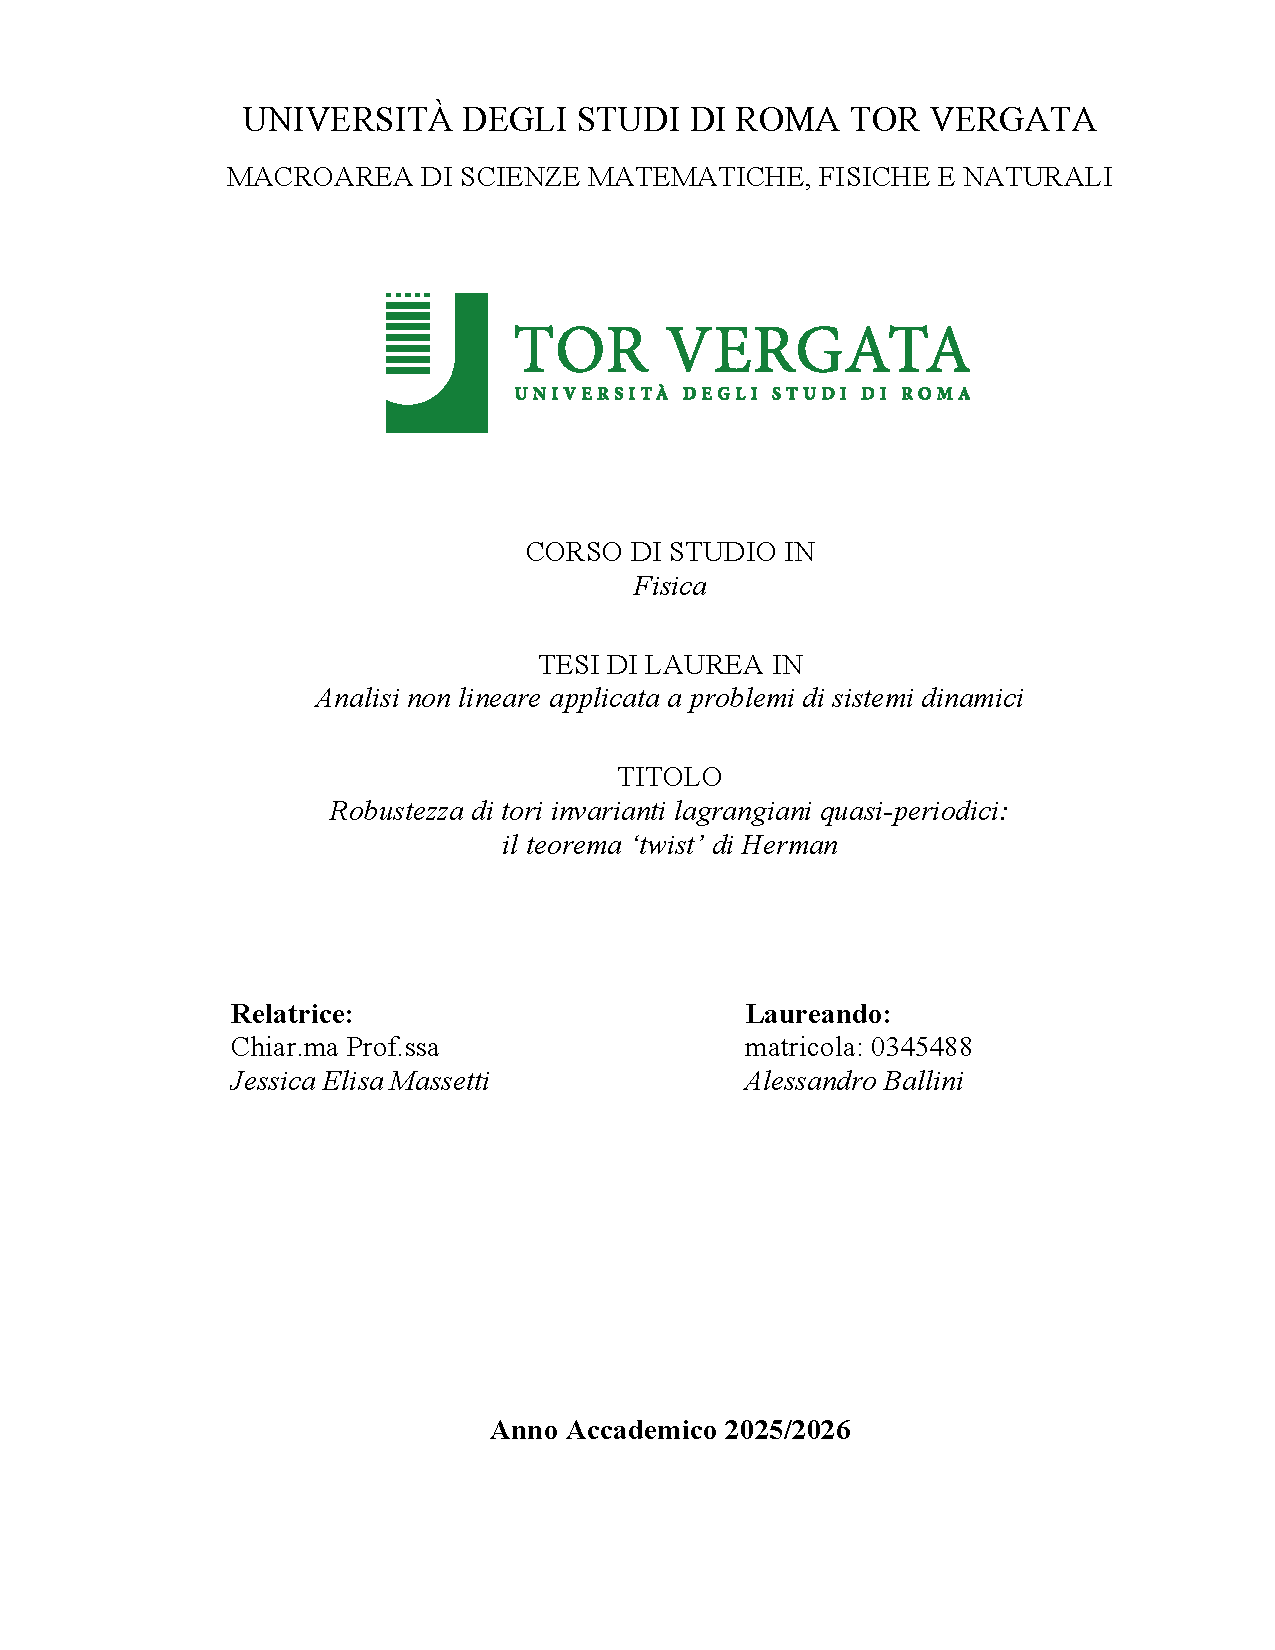
\includepdf[pages=-]{frontespizio.pdf}
\maketitle
\tableofcontents

\chapter*{Introduzione}
La scoperta da parte di Hook e Newton della legge di attrazione universale ribaltò, alla fine del XVII secolo, la nostra comprensione del movimento degli astri del sistema solare. Si capì molto rapidamente che le loro implicazioni puramente dinamiche erano enormi: i pianeti si perturbano mutualmente nel loro movimento ellittico kepleriano intorno al Sole. Non fu più evidente che il Sistema solare fosse stabile e da lì, nacque uno dei problemi matematici più antichi e resistenti nel tempo, quello della stabilità del sistema solare: \textit{il movimento dei pianeti si ripete immutabilmente, o al contrario possono succedere collisioni o espulsioni? } 
%Il problema di determinare la stabilità a lungo termine delle soluzioni nei sistemi dinamici affonda le proprie radici nei grandi problemi della meccanica celeste, nati con la legge di gravitazione di Newton, in particolare nel problema della stabilità del sistema solare. \\
Un avanzamento spettacolare a livello matematico fu compiuto negli anni 1950-60 quando, utilizzando i lavori di Kolmogorov, Arnold dimostrò il seguente teorema (si veda \cite{Arn63}): se le masse dei pianeti fossero state sufficientemente piccole rispetto a quella del Sole (in realtà incomparabilmente più piccole rispetto alle masse reali), per \textit{molte} (in un senso matematico preciso) condizioni iniziali (posizioni e velocità iniziali dei pianeti), il movimento dei pianeti sarebbe stato \textit{quasi-periodico}, ossia una sorta di sovrapposizione di movimenti oscillatori; in particolare, questi movimenti sono limitati e senza collisioni, esattamente come lo è la loro approssimazione kepleriana.  Detto più precisamente, nel modello newtoniano del sistema planetario, costituito dal Sole e da $n \geq 2$ pianeti, se il massimo dei rapporti tra le masse dei pianeti e la massa del Sole è sufficientemente piccolo, in un intorno nello spazio delle fasi dei moti kepleriani circolari e complanari, esiste un insieme di condizioni iniziali di misura di Lebesgue strettamente positiva che dà luogo a moti \textit{quasi-periodici}. Si tratta di un clamoroso risultato di stabilità, anche se, da un lato, non si applica al sistema solare stesso, e se, dall'altro, anche supponendo che le masse siano sufficientemente piccole, non si applica a \textit{tutte} le condizioni iniziali possibili. L'ampiezza delle difficoltà matematiche per dimostrare un tale risultato (la cui dimostrazione passa per un algoritmo di Newton rivoluzionario, in dimensione \emph{infinita}) aveva fatto arretrare matematici straordinari come Weierstrass e Poincaré. 

La teoria KAM (dal nome dei tre matematici Kolmogorov, Arnold e Moser), all'interno della quale questo lavoro di tesi si inserisce, ha per oggetto lo studio dei movimenti quasi-periodici e la loro robustezza per piccola perturbazione. Questa teoria è stata sviluppata originariamente per sistemi conservativi, generalmente Hamiltoniani, dove certe quantità, tra cui l'energia, sono conservate nel corso del tempo (la conservazione dell'energia è un'ipotesi naturale se ci aspettiamo una forma di regolarità del moto nel corso del tempo). 

La dimostrazione originale di Arnold è completa solo nel caso del problema piano dei tre corpi. 
Una dimostrazione completa del teorema è stata presentata da Herman negli anni 90, durante una serie di seminari all'Université Paris 7 ( "Démonstration d'un théorème de V.I. Arnold" - Séminaire de Systièmes Dynamiques). Egli dedusse il teorema di Arnold da un teorema astratto di tori invarianti più generale, mostrando che il sistema planetario soddisfa le sue ipotesi. In \cite{Fejoz04} Féjoz dettaglia completamente la dimostrazione esposta da Herman.
%Una dimostrazione completa e rigorosa del teorema è stata data da Herman, che nel corso degli anni '90 dimostrò un teorema astratto di \textit{tori invarianti}, generalizzando quello di Arnold, e mostrò poi che il sistema planetario rientra nelle sue ipotesi (si veda \cite{Fejoz04} per una dimostrazione). \\
L'idea alla base del risultato è la seguente. Poiché le masse dei pianeti sono molto più piccole di quella del Sole, in prima approssimazione ogni pianeta si muove su un'ellisse kepleriana, come se risentisse della sola attrazione solare, e il sistema è integrabile. Le interazioni mutue tra i pianeti si comportano come una piccola perturbazione, il cui parametro è proprio il rapporto massimo tra le masse. Il sistema planetario è dunque una perturbazione di un sistema ben noto, che sappiamo integrare esattamente, composto da $n$ corpi non interagenti che orbitano attorno ad una massa centrale fissa. \\ \\
Il risultato di Arnold è un esempio significativo di un fenomeno più generale, legato ai sistemi completamente integrabili e alle loro perturbazioni. \\
Abbandoniamo ora il caso planetario, che richiede ipotesi più delicate di quelle con cui lavoreremo in seguito, e studiamo le caratteristiche (in parte sopra citate) e i comportamententi rispetto a piccole perturbazioni di questa classe di sistemi, a partire dal modello astratto più naturale. \\ \\
Consideriamo dunque un'hamiltoniana analitica $H : \mathbb{T}^n \times \mathbb{R}^n \longrightarrow \mathbb{R}$ della forma $H(\theta, r) = H_0(r)$. \\
Un sistema descritto da un'hamiltoniana come $H$ rientra nella classe dei \textit{sistemi hamiltoniani completamente integrabili}, che prendono nome proprio dalla possibilità immediata di integrare le equazioni del moto ad essi associate e quindi determinarne le soluzioni. Il campo di velocità indotto dalle equazioni del moto di Hamilton è della forma
\begin{align}
    \begin{pmatrix}
        \dot{\theta} \\
        \dot{r}
    \end{pmatrix} = \begin{pmatrix}
        \frac{\partial H_0}{\partial r}(r) \\
        0
    \end{pmatrix} \notag
\end{align}
dove $(\dot{\theta}, \dot{r}) = (\dot{\theta}_1, \dots, \dot{\theta}_n, \dot{r}_1, \dots, \dot{r}_n)$ e
\begin{align}
    \frac{\partial H_0}{\partial r} = \left(\frac{\partial H_0}{\partial r_1}, \dots, \frac{\partial H_0}{\partial r_n}\right). \notag
\end{align}
Osserviamo che lo spazio delle fasi $\mathbb{T}^n \times \mathbb{R}^n$ è foliato da tori della forma $\mathbb{T}^n \times \{r_0\}$ invarianti per il flusso del campo di velocità hamiltoniano
\begin{align}
    \varphi_t : \begin{pmatrix}
        \theta \\
        r_0
    \end{pmatrix} \mapsto \begin{pmatrix}
        \theta + t\frac{\partial H_0}{\partial r}(r_0) \\
        r_0
    \end{pmatrix} \notag
\end{align}
che è una traslazione lineare sul toro di frequenza $\alpha = \alpha(r_0) := \frac{\partial H_0}{\partial r}(r_0)$. \\ \\
In generale dato $\alpha = (\alpha_1, \dots, \alpha_n) \in \mathbb{R}^n$ tale che $k \cdot \alpha \neq 0$ per ogni $k \in \mathbb{Z}^n \setminus \{0\}$, una soluzione $u$ associata ad una condizione iniziale nello spazio delle fasi $\mathcal{P}$ è detta $\alpha$-\textit{quasi-periodica} se esiste un embedding del toro nello spazio delle fasi
\begin{align}
    \theta \mapsto U(\theta, r_0) \notag
\end{align}
tale che $u(t) = U(\alpha t)$ per ogni $t \in \mathbb{R}$ (dominio massimale di definizione). 
Tali soluzioni consistono quindi in una sovrapposizione di moti oscillatori di $n$-frequenze indipendenti. 
Se $\alpha := \frac{\partial H_0}{\partial r}(r_0)$ è un vettore di frequenze razionalmente indipendenti, allora il flusso $\varphi_t (\theta)$ riempie densamente il toro $\mathbb{T}^n\times\{r_0\}$ (si veda proposizione \ref{NonResErgFlowEq}).

Fissiamo allora l'attenzione su un singolo toro della foliazione, ad esempio $T^n_0 := \mathbb{T}^n \times \{0\}$, supponiamo $\alpha := \frac{\partial H_0}{\partial r}(r_0)$ come sopra, e osserviamo che ogni hamiltoniana $K$ della forma
\begin{align}
    K = c + \alpha \cdot r + O(r^2) \notag
\end{align}
dove $c \in \mathbb{R}$, e $O(r^2)$ è un termine almeno quadratico nelle azioni $r$, i.e. $O(r^2) = P(\theta, r)$ che soddisfa
\begin{align}
    \begin{cases}
        P(\theta, 0) = 0 \\
        \frac{\partial P}{\partial r}(\theta, 0) = 0
    \end{cases} \notag
\end{align}
per ogni $\theta \in \mathbb{T}^n$, possiede un toro invariante $\alpha$-quasi-periodico, ovvero $T^n_0$. \\ 


A questo punto, è interessante chiedersi se il moto caratteristico dei sistemi completamente integrabili (o, più in generale, descritti da hamiltoniane come $K$) sui tori invarianti sopravvive, seppur leggermente deformato, anche per piccole perturbazioni dei sistemi stessi. \\
Pertanto consideriamo un'hamiltoniana $H$ analitica della forma
\begin{align}
    H(\theta, r) = H_0(r) + \varepsilon H_1(\theta, r) + \varepsilon^2H_2(\theta, r) + O(\varepsilon^3) \notag 
\end{align}
dove $0 \leq \varepsilon \ll 1$. L'hamiltoniana $H$ descrive un \textit{sistema hamiltoniano quasi integrabile}, ovvero una piccola perturbazione di un sistema completamente integrabile, infatti, per $\varepsilon = 0$, si ottiene $H(\theta, r) = H_0(r)$. \\
Storicamente, l'approccio risolutivo consisteva nel cercare di rimuovere la dipendenza dalla variabile del moto $\theta$ per il termine di ordine $\varepsilon$, tramite opportuni cambi di coordinate, e, in caso di successo, procedere iterativamente per ogni ordine successivo in $\varepsilon$. \\
Tale procedimento prevede, ad ogni passo, la risoluzione su $\mathbb{T}^n$ di equazioni della forma
\begin{align}
    \mathcal{L}_\alpha f = g - g_0 \notag 
\end{align}
detta \textit{equazione omologica}, dove $\alpha = \sum a_j\frac{\partial}{\partial \theta_j}$ è il campo di velocità hamiltoniano costante sul toro invariante, $\mathcal{L}_\alpha$ l'operatore derivata di Lie, $g$ una funzione nota di media $g_0$ ed $f$ la soluzione da determinare. \\ 
Viene naturale cercare $f$ in termini di serie formali di Fourier prive di termine costante. Pertanto, scrivendo
\begin{align}
    f = \sum_{k \neq 0} f_k e^{ik \cdot \theta} \qquad g = \sum_{k \neq 0} g_k e^{ik \cdot \theta} \notag 
\end{align}
si ottiene come soluzione formale
\begin{align}
    f = \sum_{k \neq 0} \frac{g_k}{ik \cdot \alpha} e^{ik \cdot \theta} \notag 
\end{align}
Inizialmente si pensava che fosse sufficiente supporre che $\alpha$ fosse \textit{non risonante}, ovvero che $k \cdot \alpha \neq 0$ per ogni $k \in \mathbb{Z}^n \setminus \{0\}$, per garantire la convergenza delle serie perturbative classiche. \\
Tuttavia, in seguito, Poincaré dimostrò che si trattava in realtà di serie divergenti a causa dell'accumulo a $0$, al variare di $k\in\Z^n$, dei termini $k \cdot \alpha$, detti per l'appunto \textit{piccoli divisori} ($\inf_k |k \cdot \alpha| = 0$). \\ 
Fu poi Kolmogorov ad aggiungere l'ipotesi di \textit{forte non risonanza}, i.e. una condizione aritmetica sul vettore frequenza $\alpha$ che desse una stima dal basso, necessariamente dipendente da $k$, richiedendo che
\begin{align}
    |k \cdot \alpha| \geq \frac{\gamma}{|k|^\tau} \notag
\end{align}
per ogni $k \in \mathbb{Z}^n \setminus \{0\}$, dove $\gamma > 0$ e $\tau > n - 1$. Tali vettori $\alpha$ sono detti $(\gamma, \tau)$-\textit{diofantei}. In particolare, si può dimostrare (si veda la proposizione \ref{DiofSubsetFullMeasure}) che il sottoinsieme di $\mathbb{R}^n$ composto dai vettori $(\gamma, \tau)$-diofantei, per qualche $\gamma > 0$, ha misura di Lebesgue piena, ovvero quasi tutti i vettori di $\mathbb{R}^n$ soddisfano tale condizione. \\ \\
Supponendo vettore frequenza $\alpha$ diofanteo ed opportune condizioni di non degenerazione sul termine quadratico di $K$, nel 1954 Kolmogorov dimostrò la persistenza di tori invarianti $\alpha$-quasi-periodici per piccole perturbazioni  (si veda il teorema \ref{KolmThmStrongNonDeg}):
\begin{thm}[Kolmogorov]
dati $\alpha$ diofanteo e $K^0 = c + \alpha \cdot r + \frac{1}{2}Qr \cdot r + O(r^3)$ con $Q$ forma quadratica non degenere, per ogni $H$ sufficientemente vicino a $K^0$ esistono unici $K = c + \alpha \cdot r + O(r^2)$ vicino a $K^0$ e $G$ opportuno cambio di coordinate simplettico vicino all'identità tali che
\begin{align}
    H = K \circ G \notag
\end{align}
in un intorno di $T^n_0$.
\end{thm}
Tale teorema mostra quindi che $G^{-1}(T^n_0)$ è un toro invariante $\alpha$-quasi-periodico per $H$. \\ \\
L'idea di Kolmogorov consisteva nel fissare un vettore frequenza $\alpha$ diofanteo e cercare una correzione delle azioni e una deformazione del toro tali che il sistema perturbato conservasse la dinamica $\alpha$-quasi-periodica sul toro deformato. \\
In particolare, ideò uno schema iterativo ispirato al metodo della tangente di Newton, caratterizzato da una \textit{superconvergenza}, con errore residuo all'$m$-esimo passo dell'ordine di $\varepsilon^{\chi^m}$, $1 < \chi < 2$. Questo metodo gli permise di controllare le perdite di analiticità dovute alla risoluzione delle equazioni omologiche ad ogni passo dello schema iterativo alla Newton (si veda la proposizione \ref{HomEq&CauchyEst}) e quindi di garantire la convergenza della successione costruita. \\ \\
Nel corso degli anni '90, Herman in \cite{Herman} propose un'ulteriore dimostrazione del teorema di Kolmogorov usando un approccio più flessibile e generale (la cui essenza è la stessa con cui dimostrò il teorema di Arnold), che gli permise di dimostrare il problema originale in due passi principali. \\
\textbf{1.} Fissato $\alpha$ diofanteo e senza supporre alcuna condizione di non degenerazione su $K^0$, si modifica opportunamente $H$ introducendo un controtermine $\beta \cdot r$, per qualche $\beta \in \mathbb{R}^n$ da determinare, in modo da poterlo coniugare, tramite un cambio di coordinate $G$ da determinare, ad un'hamiltoniana $K$ che possiede un toro invariante $\alpha$-quasi-periodico, per mostrare che $H$ modificata soddisfa la seguente \textit{forma normale}
\begin{align}
    H - \beta \cdot r = K \circ G. \notag
\end{align}
Chiaramente, il termine $\beta \cdot r$ ostruisce la coniugazione dinamica tra $H$ e $K$ (Herman la battezzò quindi \textit{conjugaison tordue}, in inglese \textit{twisted conjugacy}). \\
Questo passaggio è quello che contiene tutta l'\textit{analisi dura} del problema, ovvero tutte le difficoltà tecniche principali. Infatti, si tratta sempre di applicare uno schema iterativo alla Newton, come fece Kolmogorov, per dimostrare che l'operatore non lineare
\begin{align}
    \phi : (K, G, \beta) \mapsto H = K \circ G + \beta \cdot r \notag
\end{align}
è invertibile localmente, in un intorno di $(K^0, \mathrm{id}, 0)$ (si veda \ref{SettingFunz} per una definizione precisa degli spazi funzionali coinvolti). \\
Il problema di dimostrare la persistenza di $T^n_0$ per $H$ è ora ridotto a un problema di dimensione finita: eliminare $\beta \in \mathbb{R}^n$. \\
\textbf{2.} Una volta risolto il primo passaggio, se $H$ dipende da un numero sufficiente di parametri liberi e $\beta$ ne dipende in modo regolare, possiamo sperare di risolvere $\beta = 0$ tramite un teorema classico della funzione inversa. \\
Nel caso specifico di Kolmogorov, la condizione di non degenerazione su $Q$ garantisce che $\beta = \beta(r)$ sia differenziabile nelle azioni $r$ (che possiamo usare come parametri liberi) e che $\frac{\partial \beta}{\partial r}(r)$ è invertibile. \\ \\
In realtà, l'idea di separare il problema in due passaggi nacque da Arnold, durante lo studio delle rotazioni del cerchio
\begin{align}
    f : \mathbb{T} \longrightarrow \mathbb{T} \qquad f(\theta) = \theta + \omega, \qquad \omega \in \mathbb{R} \notag
\end{align}
e del loro comportamento sotto piccole perturbazioni. Nel tentativo di riconiugare le perturbazioni a rotazioni di frequenza fissata $\alpha$, Arnold suddivise il problema esattamente nei due passaggi che hanno caratterizzato poi il metodo impiegato da Herman nella dimostrazione del suo teorema. \\ \\
In questo lavoro ci proponiamo di dimostrare il \textit{celebre teorema di Kolmogorov} deducendolo, appunto, dal teorema '\textit{twisted conjugacy}' di Herman (si veda il teorema \ref{TwistThmHerman2}):
\begin{thm}[Herman, \textit{twisted conjugacy}]
    dati $\alpha$ diofanteo e $K^0 = c + \alpha \cdot r + O(r^2)$, per ogni $H$ sufficientemente vicino a $K^0$ esistono unici $K$ vicino a $K^0$, $G$ cambio di coordinate simplettico esatto vicino all'identità e $\beta \in \mathbb{R}^n$ vicino all'origine tali che
\begin{align}
    H - \beta \cdot r = K \circ G \notag
\end{align}
in un intorno di $T^n_0$.
\end{thm}



\chapter{Sistemi hamiltoniani}
\section{Punto di vista geometrico}
Consideriamo una funzione liscia $H$ definita su $ T^*\mathbb{T}^n \cong \mathbb{T}^n \times \mathbb{R}^n$ = $\{(\theta, r)\}$ (dove $\mathbb{T}^n = \mathbb{R}^n/2\pi\mathbb{Z}^n$ è il toro $n$-dimensionale). \\
Il \textit{campo vettoriale hamiltoniano} $X_H$ indotto da $H$ tramite le equazioni di Hamilton è dato da 
\begin{align}\label{HamVectField}
    X_H = \begin{pmatrix}
        \dot{\theta} \\
        \dot{r}
    \end{pmatrix} =
    \begin{pmatrix}
        \frac{\partial H}{\partial r} \\
        -\frac{\partial H}{\partial \theta}
    \end{pmatrix} = J\grad H 
\end{align}
dove
\begin{align}
    J = \begin{pmatrix}
        0 & \mathbf{1} \\
        -\mathbf{1} & 0
    \end{pmatrix}
\end{align}
Notiamo immediatamente che $\nabla H \cdot X_H = 0$, il gradiente di $H$ è ortogonale al campo vettoriale hamiltoniano $X_H$, infatti $J$ è una matrice antisimmetrica. \\ \\
In particolare, la proiezione sul piano $\{(\theta_j, r_j)\}$ del campo vettoriale hamiltoniano $X_H$ e del gradiente euclideo $\nabla H$ sono ortogonali, ovvero ogni termine della somma è nullo
\begin{align}
    \nabla H \cdot X_H = \sum_j\left(\frac{\partial H}{\partial \theta_j}\frac{\partial H}{\partial r_j} - \frac{\partial H}{\partial r_j}\frac{\partial H}{\partial \theta_j}\right)
\end{align}
Pertanto $X_H$ è tangente alle curve di livello di $H$ (curve ad energia fissata), quindi $H$ è costante lungo il flusso di $X_H$. \\ \\
Tutta l'informazione riguardante un determinato sistema dinamico è contenuta nella funzione di Hamilton $H$ associata. \\
Solamente una particolare classe di cambi di coordinate è ammessa, ovvero i diffeomorfismi $\phi$ che lasciano invariata la forma di $X_H$ (e quindi delle equazioni del moto), cioè
\begin{align}\label{SymplMorph}
    \phi_*X_H = X_{H \circ \phi^{-1}} 
\end{align}
Per caratterizzare tali diffeomorfismi diamo prima una definizione instrinseca di $X_H$. Sia
\begin{align}
    \omega = \sum_j d\theta_j \wedge dr_j 
\end{align}
$\omega$ è detta \textit{forma simplettica} standard sullo spazio delle fasi $\mathbb{T}^n \times \mathbb{R}^n$. In particolare, $\omega$ è una mappa bilineare antisimmetrica e non degenere del fibrato tangente dello spazio delle fasi nella retta reale. \\
Dato $X = (\dot{\theta}, \dot{r})$ campo vettoriale su $\mathbb{T}^n \times \mathbb{R}^n$, si ha
\begin{align}\label{iota_X omega}
    \iota_X\omega = \sum_j (\dot{\theta}_jdr_j - \dot{r}_jd\theta_j) 
\end{align}
Segue che $X_H$ è definito implicitamente dall'equazione
\begin{align}\label{X_H ImplDefn}
    \iota_{X_H}\omega = dH 
\end{align}
In generale, possiamo dire che $X_H$ è un campo vettoriale 'hamiltoniano' se esiste $H$ che soddisfa \eqref{X_H ImplDefn}, in tal caso, confrontando con \eqref{iota_X omega}, $X_H$ è caratterizzato da \eqref{HamVectField}. \\ \\
Poniamo $\eta = (\theta, r)$, dato $\phi : \eta \mapsto \phi(\eta) =: z$ diffeomorfismo e $H$ hamiltoniana, vogliamo determinare che forma deve avere $\phi$ affinché anche $K := H \circ \phi^{-1}$ sia hamiltoniana, ovvero affinché valga
\begin{align}\label{KHam}
    \dot{z} = J\nabla_z K
\end{align}
Per ipotesi $H$ è hamiltoniana, pertanto
\begin{align}
    \dot{\eta} = J\nabla_\eta H
\end{align}
Mentre, in generale, si avrà
\begin{align}
    \dot{z} = \phi'(\eta)\dot{\eta} = \phi' \circ \phi^{-1} \, (z) J\nabla_\eta H \circ \phi^{-1}(z)
\end{align}
e
\begin{align}
    J\nabla_z K = J\nabla_\eta H \circ \phi^{-1}(z)\phi'^{-1} \circ \phi^{-1}(z)
\end{align}
Pertanto \eqref{KHam} è soddisfatta se
\begin{align}\label{SymplCond}
    \phi'(\eta)J = J\null^t\phi'(\eta)^{-1}
\end{align}
per ogni $\eta$. \\
Poiché $\omega(X, Y) = \null^t X J Y$, si ottiene che le uniche trasformazioni che preservano la forma delle equazioni di Hamilton sono le trasformazioni che soddisfano
\begin{align}
    \phi^*\omega = \omega
\end{align}
Infatti, per definizione di pullback di un forma differenziale, si ha
\begin{align}
    \phi^*\omega(X, Y) = \null^t(\phi' X)J(\phi' Y) = \null^tX \null^t\phi' J \phi' Y = \null^tX J Y = \omega(X, Y)
\end{align}
se \eqref{SymplCond} è soddisfatta. Tali trasformazioni sono dette \textit{simplettiche} o \textit{canoniche}.
\begin{ex} consideriamo una $1$-forma differenziale chiusa $\rho$ su $\mathbb{T}^n$
\begin{align}
    \rho = \sum_i \rho_i(\theta)d\theta_i \qquad d\rho = 0 
\end{align}
dove $\rho_i : \mathbb{T}^n \longrightarrow \mathbb{R}$ almeno di classe $C^1$, $i = 1, \dots, n$. Il diffeomorfismo $\phi$ definito da 
\begin{align}
    (\theta, r) \mapsto (\theta, r + \rho(\theta)) 
\end{align}
dove $\rho(\theta) = (\rho_1(\theta), \dots, \rho_n(\theta))$, per $\theta \in \mathbb{T}^n$, è simplettico. Infatti
\begin{align}
    \phi^*\omega = \sum_j d\tilde{\theta}_j \wedge d\tilde{r}_j 
\end{align}
dove si è posto $\tilde{\theta} = \theta$ e $\tilde{r} = r + \rho$, segue che $d\tilde{\theta}_j = d\theta_j$ e $d\tilde{r}_j = dr_j + d\rho_j$ per ogni $j = 1, \dots, n$. Pertanto
\begin{align}
    \phi^*\omega &= \sum_j d\theta_j \wedge (dr_j + d\rho_j) \\
    &= \sum_j d\theta_j \wedge dr_j + \sum_j d\theta_j \wedge d\rho_j \\
    &= \omega - d\rho = \omega 
\end{align}
dato che $d\rho = 0$ per ipotesi.
\end{ex}
\begin{ex} sia $\varphi$ un diffeomorfismo su $\mathbb{T}^n$. Definiamo il sollevamento $\phi$ di $\varphi$ al fibrato cotangente di $\mathbb{T}^n$
\begin{align}\label{ContraGrad}
    \phi: \quad (\theta, r) \mapsto \underbrace{(\varphi(\theta), r\varphi'(\theta)^{-1})}_{(\tilde{\theta}, \tilde{r})}
\end{align}
dove con $\varphi' = D\phi$ (jacobiano). Il diffeomorfismo $\phi$ preserva la $1$-\textit{forma di Liouville} $\lambda = \sum_j r_jd\theta_j$, infatti
\begin{align}
    \phi^*\lambda = \tilde{r} \cdot d\tilde{\theta} = r \cdot \varphi'(\theta)^{-1}\varphi'(\theta) \cdot d\theta = \lambda
\end{align}
Inoltre, dato che $d\lambda = -\omega$, si ha
\begin{align}\label{PhiSympl}
    \phi^*\omega = -\phi^*d\lambda = -d\phi^*\lambda = -d\lambda = \omega
\end{align}
dove si è usato che le operazioni di pullback e di differenziazione esterna commutano. Pertanto $\phi$ simplettico.
\end{ex}
\begin{defn} sia $M$ una varietà di dimensione $2n$, una sottovarietà $L$ è detta \textit{lagrangiana} se $\dim L = n$ e la  $2$-forma simplettica si annulla su $L$.
\end{defn}
\begin{rmk} $\mathbb{T}^n \cong \mathbb{T}^n \times \{0\} \subset \mathbb{T}^n \times \mathbb{R}^n$ è una sottovarietà lagrangiana, infatti $\dim \mathbb{T}^n \times \{0\} = n$ e $\omega|_{\mathbb{T}^n \times \{0\}} = 0$ proprio perché $dr_i(v) = 0$ per ogni $v \in T_{(\theta, 0)}\mathbb{T}^n$, per ogni $i = 1, \dots, n$.
\end{rmk}
\begin{lemma}
Data $\phi$ come in \eqref{ContraGrad}, le seguenti sono equivalenti: \\
\textbf{1.} il grafico di $\rho : \mathbb{T}^n \longrightarrow \mathbb{R}^n$ ($\subset T^*\mathbb{T}^n \cong \mathbb{T}^n \times \mathbb{R}^n$) è una sottovarietà lagrangiana. \\
\textbf{2.} la forma di Liouville $\sum_j \rho_j \, d\theta_j$ su $\mathbb{T}^n$ è chiusa. \\
\textbf{3.} la mappa $(\theta, r) \mapsto (\theta, r + \rho(\theta))$ è simplettica.
\end{lemma}
\begin{proof}
($1 \rightarrow 2$) segue immediatamente dalla definizione di varietà lagrangiana. \\
($2 \rightarrow 3$) lo abbiamo visto in \eqref{PhiSympl}. \\
($3 \rightarrow 1$) perché il fatto che $(\theta, r) \mapsto (\theta, r + \rho(\theta))$ è simplettica implica che $d\rho = 0$ e $d\rho$ non è altro che la $2$-forma simplettica definita sul grafico di $\rho$, che è $\{(\theta, \rho(\theta))\}$.
\end{proof}
\begin{lemma}[\cite{Bost}]\label{LemBost} se $Gr \, \rho$, grafico di $\rho$, è una sottovarietà lagrangiana di $\mathbb{T}^n \times \mathbb{R}^n$, data $H$ hamiltoniana definita su un aperto di $Gr \, \rho$, è necessario e sufficiente che $H$ sia costante su $Gr \, \rho$ affinché $Gr \, \rho$ sia invariante per il flusso hamiltoniano di $H$.
\end{lemma}

\begin{proof} dato $p \in Gr \, \rho$ poniamo
\begin{align}
    (T_pGr \, \rho)^\omega = \{v \in T_p \, \mathbb{T}^n \times \mathbb{R}^n : \omega_p(u, v) = 0 \text{ per ogni } u \in T_pGr \, \rho\}
\end{align}
detto \textit{ortogonale simplettico}. Per ipotesi $Gr \, \rho$ è una sottovarietà lagrangiana, quindi $\omega|_{Gr \rho} = 0$, segue che $T_pGr \, \rho = (T_pGr \, \rho)^\omega$, dato che $\omega$ è non degenere. Inoltre
\begin{align}
    \iota_{X_H}\omega_p(v) = dH_p(v) = 0
\end{align}
per ogni $v \in T_pGr \, \rho$, dato che $H$ è costante su $Gr \, \rho$, per ipotesi. Segue che $X(p) \in T_pGr \, \rho$ per ogni $p \in Gr \, \rho$, quindi $Gr \, \rho$ invariante per il flusso di $X_H$. 
\end{proof}
\begin{rmk} una qualsiasi sottovarietà lagrangiana $L$ su cui $H$ è costante soddisfa $T_pL = (T_pL)^\omega$ per ogni $p$ in $L$. Inoltre, se $H$ è costante su $L$, $L$ è invariante per il flusso generato da $X_H$.
\end{rmk}
\begin{prop} sia $\phi_t$ è il flusso associato ad un campo vettoriale hamiltoniano $X_H$, allora $\phi^*_t\omega = \omega$ per ogni $t$ nell'intervallo di definizione del flusso.
\end{prop}

\begin{proof} per il \textit{teorema fondamentale del calcolo} si ha
\begin{align}
    \phi^*_t\omega - \omega &= \int_0^t \frac{d}{ds}(\phi^*_s\omega) \, ds \notag \\
    &= \int_0^t \left.\frac{d}{d\tau}\right|_{\tau = 0}(\phi^*_{s + \tau}\omega) \, ds \notag \\
    &= \int_0^t \left.\frac{d}{d\tau}\right|_{\tau = 0}(\phi^*_s\phi^*_\tau \omega) \, ds \notag \\
    &= \int_0^t \phi^*_s\left.\frac{d}{d\tau}\right|_{\tau = 0}(\phi^*_\tau \omega) \, ds \notag \\
    &= \int_0^t \phi^*_s(\mathcal{L}_{X_H}\omega) \, ds
\end{align}
Per la \textit{formula magica di Cartan} (cfr. \cref{CartanFormula}) si ha
\begin{align}
    \mathcal{L}_{X_H}\omega = di_{X_H}\omega + i_{X_H}d\omega
\end{align}
In particolare, $d\omega = 0$, dato che che $\omega$ ha tutti coefficienti costanti, mentre $i_{X_H}\omega = dH$, pertanto $di_{X_H}\omega = d^2H = 0$ (dato che $d^2 = 0$, \textit{operatore di coomologia}). 
\end{proof}

\chapter{Sistemi completamente integrabili}
Studiamo ora una classe particolare di sistemi hamiltoniani: i sistemi hamiltoniani \textit{completamente integrabili}. \\
Un sistema hamiltoniano è detto completamente integrabile se $H(\theta, r) = h(r)$ per ogni $(\theta, r)$ nello spazio delle fasi. In tal caso si ottiene 
\begin{align}
    \begin{cases}
        \dot{\theta} &= \frac{\partial h}{\partial r} = cst \\
        \dot{r} &= 0
    \end{cases} 
\end{align}
\section{Campi vettoriali costanti sul toro}
Possiamo facilmente determinare il flusso associato a $X_H$ 
\begin{align}
    \phi_t(\theta, r) = \left(\theta + t\frac{\partial h}{\partial r}(r), r\right) 
\end{align}
per ogni $t \in \mathbb{R}$ (intervallo massimale di definizioni delle soluzioni). \\
Notiamo che lo spazio delle fasi è foliato da tori invarianti, infatti fissato $r_0 \in \mathbb{R}^n$ si ha 
\begin{align}
    \phi_t\left(\mathbb{T}^n \times \{r_0\}\right) = \mathbb{T}^n \times \{r_0\} 
\end{align}
Il flusso ristretto ad uno qualsiasi dei tori invarianti è \textit{quasi-periodico} con \textit{vettore frequenza} $\alpha(r_0) = \frac{\partial h}{\partial r}(r_0) \in \mathbb{R}^n$.
\begin{ex}
Consideriamo $H : \mathbb{R}^{2} \longrightarrow \mathbb{R}$ definita da
\begin{align}
    H(p, q) = \frac{p^2 + q^2}{2}
\end{align}
essenzialmente l'hamiltoniana dell'oscillatore armonico unidimensionale. \\
Vogliamo trovare un cambio di coordinate simplettico
\begin{align}
    \phi : (p, q) \mapsto (\theta, r)
\end{align}
che renda $H$ completamente integrabile, ovvero tale che
\begin{align}
    \phi^*H = h(r)
\end{align}
Osserviamo che
\begin{align}
    \phi : (p, q) \mapsto (p(\theta, r), q(\theta, r)) = (\sqrt{2r}\sin\theta, \sqrt{2r}\cos\theta)
\end{align}
dove
\begin{align}
    r^2 = p^2 + q^2 \qquad \theta = \arcsin \frac{r}{p}
\end{align}
è simplettico, infatti
\begin{align}
    \phi^*(dp \wedge dq) &=  d(p \circ \phi) \wedge d(q \circ \phi) \notag \\
    &= \left(\frac{\partial p}{\partial \theta}d\theta + \frac{\partial p}{\partial r}dr\right) \wedge \left(\frac{\partial q}{\partial \theta}d\theta + \frac{\partial q}{\partial r}dr\right) \notag \\
    &= \left(\frac{\partial p}{\partial \theta}\frac{\partial q}{\partial r} - \frac{\partial p}{\partial r}\frac{\partial q}{\partial \theta}\right)d\theta \wedge dr \notag \\
    &= \{p, q\}d\theta \wedge dr
\end{align}
dove $\{p, q\}$ sono le parentesi di Poisson calcolate per le nuove coordinate $p = p(\theta, r)$ e $q = q(\theta, r)$. \\
Osserviamo che
\begin{align}
    \{p, q\} = \sqrt{2r}\cos\theta \cdot \frac{1}{\sqrt{2r}}\cos\theta + \frac{1}{\sqrt{2r}}\sin\theta \cdot \sqrt{2r}\sin\theta = 1
\end{align}
Pertanto $\phi^*(dp \wedge dq) = d\theta \wedge dr$, quindi $\phi$ simplettico. \\
Inoltre, si vede immediatamente sostituendo che $\phi^*H = h(r) = r$, completamente integrabile.
\end{ex}
Fissiamo $r_0 \in \mathbb{R}^n$ e consideriamo il flusso lineare
\begin{align}
    \varphi_t : \mathbb{T}^n \longrightarrow \mathbb{T}^n \qquad \theta \mapsto \theta + t\alpha \notag
\end{align}
dove $\alpha = \frac{\partial h}{\partial r}(r_0)$. \\
Diciamo che $\varphi^\alpha_t, \varphi^\beta_t$ (flussi associati a due sistemi completamente integrabili con vettori frequenza $\alpha, \beta$) sono \textit{topologicamente coniugati} (cfr. definizione \ref{TopConjDefn}) se esiste $h$ omeomorfismo di $\mathbb{T}^n$ tale che il seguente diagramma commuta
\[
\begin{tikzcd}
\mathbb{T}^n
    \arrow[r, "\varphi^\alpha_{t}"]
    \arrow[d, "h"]
&
\mathbb{T}^n
    \arrow[d, "h"]
\\
\mathbb{T}^n
    \arrow[r, "\varphi^\beta_t"]
&
\mathbb{T}^n
\end{tikzcd}
\]
\begin{lemma}\label{FlowTopConj} il vettore frequenza $\alpha$ è invariante per coniugazione topologica a meno di azione di elementi di $GL_n(\mathbb{Z})$: se due flussi $\theta \mapsto \theta + t\alpha$ e $\theta \mapsto \theta + t\beta$, con $\alpha, \beta \in \mathbb{R}^n$, sono topologicamente coniugati, esiste $A \in GL_n(\mathbb{Z})$ tale che $\alpha = A\beta$. In particolare, se l'omeomorfismo che li coniuga preserva l'orientamento si ha $A \in SL_n(\mathbb{Z})$.
\end{lemma}

\begin{proof} supponiamo che i flussi $\theta \mapsto \theta + t\alpha$ e $\theta \mapsto \theta + t\beta$ siano topologicamente coniugati. Per definizione esiste un omeomorfismo $h$ di $\mathbb{T}^n$ tale che 
\begin{align}
    h(\theta + t\alpha) = h(\theta) + t\beta 
\end{align}
A meno di sostituire $h(\theta)$ con $h(\theta) - h(0)$, possiamo supporre $h(0) = 0$. Sia $H : \mathbb{R}^n \longrightarrow \mathbb{R}^n$ l'unico sollevamento (cfr. \cref{UniqueLift}) di $h$ tale che $H(0) = 0$. Allora 
\begin{align}\label{PhiLift}
    H(\theta + t\alpha) = H(\theta) + t\beta 
\end{align}
è soddisfatta per $\theta = 0$ e $t = 0$. Sia $\pi : \mathbb{R}^n \longrightarrow \mathbb{T}^n$ la proiezione canonica, per definizione di sollevamento
\begin{align}
    \pi(H(\theta + t\alpha)) = \pi(H(\theta) + t\beta) 
\end{align}
 per ogni $\theta \in \mathbb{R}^n$ e ogni $t \in \mathbb{R}$. Concludiamo che 
\begin{align}
    H(\theta + t\alpha) - H(\theta) - t\beta \in \mathbb{Z}^n 
\end{align}
per ogni $\theta \in \mathbb{R}^n$ e ogni $t \in \mathbb{R}$, dato che $\pi$ è una mappa $\mathbb{Z}^n$-periodica. \\
Fissato $t \in \mathbb{R}$, sia $\Delta_H$ la mappa
\begin{align}
    \theta \mapsto H(\theta + t\alpha) - H(\theta) - t\beta 
\end{align}
Notiamo immediatamente che $\Delta_H$ è continua, infatti $H$ è continua. Inoltre, dato che $\mathbb{R}^n$ è connesso, $\Delta_H$ continua e $\mathbb{Z}^n$ uno spazio con topologia discreta, concludiamo che $\Delta_H$ è costante. Pertanto \eqref{PhiLift} è soddisfatta per ogni $\theta \in \mathbb{R}^n$ (e ogni $t \in \mathbb{R}^n$). \\ \\
Notiamo che esiste $A \in GL_n(\mathbb{Z})$ tale che
 \begin{align}
    H(\theta + k) = H(\theta) + Ak 
 \end{align}
per ogni $k \in \mathbb{Z}^n$. Infatti, per definizione di sollevamento, si ha
\begin{align}
    \pi(H(\theta + k)) = h(\pi(\theta + k)) = h(\pi(\theta)) = \pi(H(\theta))
 \end{align}
ovvero
\begin{align}
    H(\theta + m) - H(\theta) \in \mathbb{Z}^n
 \end{align}
ed è costante per ogni $\theta \in \mathbb{R}^n$ (si verifica analogamente a come fatto per $\Delta_H$). \\
$A$ è invertibile, perché $H$ lo è. Consideriamo il campo vettoriale
\begin{align}
    V := A^{-1}H - \mathbf{1} : \mathbb{R}^n \longrightarrow \mathbb{R}^n
\end{align}
$V$ è $\mathbb{Z}^n$-periodico, infatti, dato $\theta \in \mathbb{R}^n$, si ha
\begin{align}
    V(\theta + m) &= (A^{-1}H - \mathbf{1})(\theta + m) \notag \\
    &= A^{-1}H(\theta + m) - \theta + m \notag \\
    &= A^{-1}H(\theta) + m - \theta + m \notag \\
    &= (A^{-1}H - \mathbf{1})(\theta) \notag \\
    &= V(\theta)
\end{align}
per ogni $m \in \mathbb{Z}^n$. Riscrivendo \eqref{PhiLift} in termini di $V$ si ottiene
\begin{align}
    (AV + A)(\theta + t\alpha) = (AV + A)(\theta) + t\beta
\end{align}
ovvero
\begin{align}
    AV(\theta + t\alpha) - AV(\theta) = t(\beta - A\alpha)
\end{align}
In particolare, per $\theta = 0$, si ha
\begin{align}
    A(V(t\alpha) - V(0)) = t(\beta - A\alpha)
\end{align}
Il membro di sinistra è limitato (dato che $V$ è $\mathbb{Z}^n$-periodico), allora deve valere $\beta = A\alpha$. \end{proof}
\section{Moti quasi-periodici}
\begin{prop}\label{NonResErgFlowEq} le seguenti affermazioni sono equivalenti: \\
\textbf{1.} Il vettore frequenza $\alpha$ è \textit{non risonante}, ovvero $k \cdot \alpha \neq 0$ per ogni $k \in \mathbb{Z}^n \setminus \{0\}$. \\
\textbf{2.} Il flusso $\varphi_t$ del campo vettoriale costante $\alpha$ è \textit{ergotico}, ovvero tutte le funzioni continue $f$ di $\mathbb{T}^n$ che soddisfano
\begin{align}
    f(\theta + t\alpha) = f(\theta)
\end{align}
per ogni $\theta \in \mathbb{T}^n$ e ogni $t \in \mathbb{R}$, ovvero le funzioni invarianti per $\varphi_t$, sono costanti. \\
\textbf{3.} Per ogni funzione continua su $\mathbb{T}^n$ esiste la media temporale $\overline{f}$ e combacia con la media spaziale su $\mathbb{T}^n$, ovvero
\begin{align}\label{time/spaceMean}
    \lim_{T \rightarrow \infty}\frac{1}{T}\int_0^T f(\theta + t\alpha) \, dt = \int_{\mathbb{T}^n} f(\theta) \, d\theta
\end{align}
considerando misura normalizzata sul toro. \\
\textbf{4.} Ogni traiettoria di $\varphi_t$ è densa in $\mathbb{T}^n$.
\end{prop}

\begin{proof} $(1 \rightarrow 2)$ sia $f$ una funzione di $\mathbb{T}^n$ tale che $f \circ \varphi_t = f$ per ogni $t \in \mathbb{R}$. Il $k$-esimo coefficiente di Fourier di $f \circ \varphi_t$ è dato da 
\begin{align}\label{k-thFCoeff}
    \widehat{f \circ \varphi_t}(k) = \int_{\mathbb{T}^n} e^{-i k \cdot \theta}f(\theta + t\alpha) \, d\theta
\end{align}
Poniamo $\theta' = \theta + t\alpha$, allora $\theta = \theta' - t\alpha$ e $d\theta = d\theta'$. Sostituendo in \eqref{k-thFCoeff} si ottiene
\begin{align}
    \widehat{f \circ \varphi_t}(k) = e^{i k \cdot \alpha t}\int_{\mathbb{T}^n} e^{-i k \cdot \theta'}f(\theta') \, d\theta' = e^{i k \cdot \alpha t}\widehat{f}(k)
\end{align}
Per ipotesi $k \cdot \alpha \neq 0$ per ogni $k \in \mathbb{Z}^n \setminus \{0\}$, pertanto, per unicità dei coefficienti di Fourier, concludiamo che $\widehat{f}(k) = 0$ per ogni $k \in \mathbb{Z} \setminus \{0\}$, quindi $f$ costante. \\ \\
$(2 \rightarrow 1)$ Supponiamo che esista $k \in \mathbb{Z}^n \setminus \{0\}$ tale che $k \cdot \alpha = 0$. Allora la funzione $f$, definita da
\begin{align}
    f(\theta) = e^{i k \cdot \theta}
\end{align}
per ogni $\theta \in \mathbb{R}^n$, è invariante ma non costante, pertanto si ottiene un assurdo. \\ \\
$(1 \rightarrow 3)$ Se $f$ è costante \eqref{time/spaceMean} è immediatamente verificata. Se $f$ è della forma
\begin{align}\label{e^iktheta}
    f(\theta) = e^{i k \cdot \theta}
\end{align}
per ogni $\theta \in \mathbb{R}^n$, con $k \in \mathbb{Z}^n \setminus \{0\}$, si ottiene
\begin{align}\label{ImmExpMean}
    \frac{1}{T}\int_0^T f(\theta + t\alpha) \, dt &= \frac{1}{T}e^{i k \cdot \theta}\int_0^T e^{i k \cdot \alpha t} \, dt \notag \\
    &= \frac{1}{T}e^{i k \cdot \theta}\frac{e^{i k \cdot aT} - 1}{ik \cdot \alpha} \rightarrow 0
\end{align}
per $T \rightarrow \infty$, ovvero la media temporale è nulla come la media spaziale (per simmetria del toro $n$-dimensionale e disparità della funzione $f$). \\
Se $f$ è un polinomio trigonometrico può essere espressa come somma finita di termini della forma $e^{i m \cdot \theta}$, per $m \in \mathbb{Z}^n$. Pertanto \eqref{time/spaceMean} è verificata grazie a \eqref{ImmExpMean} per linearità dell'integrale. \\
Per il \textit{teorema di Stone-Weierstrass} (cfr. \cite{Pedersen}), se $f$ è continua, fissato $\varepsilon > 0$, esiste $P$ polinomio trigonometrico tale che
\begin{align}
    \max_{\theta \in \mathbb{T}^n} |f(\theta) - P(\theta)| < \varepsilon
\end{align}
In particolare, per polinomi trigonometrici abbiamo appena dimostrato che 
\begin{align}
    \left|\frac{1}{T}\int_0^T P(\theta + t\alpha) \, dt\right| \rightarrow 0
\end{align}
per $T \rightarrow \infty$. Indichiamo con $\overline{\cdot}$ l'operazione di media spaziale, allora
\begin{align}
    \left|\frac{1}{T}\int_0^T f(\theta + t\alpha) \, dt - \overline{f}\right| &\leq \frac{1}{T}\int_0^T \left|f(\theta + t\alpha) - P(\theta + t\alpha)\right| \, dt \, + \notag \\
    &+ \left|\frac{1}{T}\int_0^T P(\theta + t\alpha) \, dt - \overline{P}\right| \, + \notag \\
    &+ \left|\overline{P} - \overline{f}\right| < 3\varepsilon
\end{align}
per $T$ sufficientemente grande. \\ \\
$(3 \rightarrow 1)$ Supponiamo che esista $k \in \mathbb{Z}^n \setminus \{0\}$ tale che $k \cdot \alpha = 0$. Allora $f$ definita in \eqref{e^iktheta} è una funzione invariante e continua che ha media temporale diversa dalla media spaziale, infatti
\begin{align}
    \frac{1}{T}\int_0^T e^{i k \cdot (\theta + \alpha t)} \, dt = e^{i k \cdot \theta}
\end{align}
mentre $\overline{f} = 0$. \\ \\
$(1 \rightarrow 4)$ Supponiamo che $\varphi_t$ ammetta una traiettoria \textit{non} densa. Allora esiste $\theta_0 \in \mathbb{T}^n$ che possiede un intorno aperto $U$ che non interseca con la traiettoria. \\
Consideriamo una funzione continua $f$ definita su $\mathbb{T}^n$ tale che $f(\theta) > 0$ per ogni $\theta \in U$ e $f(\theta) = 0$ per ogni $\theta \in \mathbb{T}^n \setminus U$. La media temporale di $f$ calcolata lungo la traiettoria non densa è nulla, mentre la media spaziale di $f$ è strettamente positiva. Pertanto, per il punto $(3)$ prima dimostrato, si ottiene un assurdo. \\ \\
$(4 \rightarrow 1)$ Supponiamo che esista $k \in \mathbb{Z}^n$ tale che $k \cdot \alpha = 0$. Consideriamo $\theta_0 \in \mathbb{R}^n$ tale che $k \cdot \theta_0 = 1/2 (\mod \mathbb{Z})$, mostriamo che esiste un intorno aperto $U$ di $\theta_0$ che non viene mai visitato dalla traiettoria $t \mapsto t\alpha$ su $\mathbb{T}^n$. \\
Supponiamo che esista $\theta \in U$ tale che $t\alpha = \theta$ per qualche $t \in \mathbb{R}$. Equivalentemente, esistono $t \in \mathbb{T}^n$ e $l \in \mathbb{Z}^n$ tali che $t\alpha = \theta + l$ ($\mathbb{T}^n$ è $\mathbb{Z}^n$-periodico). Facendo il prodotto scalare con $k$ si ottiene
\begin{align}
    0 = k \cdot \theta + k \cdot l
\end{align}
Tuttavia, possiamo scegliere $U$ in modo tale che $0 < |k \cdot \theta| < 1$, mentre $k \cdot l \in \mathbb{Z}$, pertanto si ottiene un assurdo.
\end{proof}
L'ergodicità della del flusso lineare $\varphi_t$, e quindi la possibilità di scambiare media temporale e spaziale, sarà quello che ci permetterà successivamente di poter lavorare con l'equazione omologica in modo che sia ben posta.

\section{Serie perturbativa}
Siamo ora interessati a determinare se, tramite opportuni cambi di coordinate simplettici, è possibile coniugare l'hamiltoniana perturbata ad un sistema che possiede un toro invariante $\alpha$-quasi-periodico. \\ \\
Consideriamo un hamiltoniana $H$ definita in un intorno aperto di $\mathbb{T}^n \times \{0\}$ in $\mathbb{T}^n \times \mathbb{R}^n$. Supponiamo che $H$ dipenda formalmente da un parametro $\varepsilon > 0$ nella forma
\begin{align}\label{PertSeries}
    H(\theta, r) = H_0(r) + \varepsilon H_1(\theta, r) + \varepsilon^2H_2(\theta, r) + O(\varepsilon^3) 
\end{align}
Vogliamo trovare un opportuno cambio di variabili, sufficientemente vicino all'identità ($\varepsilon$ vicino), tale da rimuovere la dipendenza di $H_1$ da $\theta$. Se ciò è possibile vogliamo estendere questo procedimento in moda tale da poter gestire anche i termine di ordine $\varepsilon$ superiore.
\subsection{Primo ordine in $\varepsilon$} Consideriamo un'hamiltoniana ausiliaria $F$ con flusso $\phi_t$. In particolare, vogliamo che $F$ sia tale che $\phi^*_1H = H \circ \phi_1$ non dipenda da $\theta$, almeno fino a termini di secondo ordine in $\varepsilon$. \\ \\
Osserviamo che
\begin{align}
    \frac{d}{dt}(\phi^*_tH) &= \left.\frac{d}{ds}\right|_{s = 0}(\phi^*_{t + s}H) \notag \\
    &= \left.\frac{d}{ds}\right|_{s = 0}(H \circ \phi_{t + s}) \notag \\
    &= \left.\left(dH \circ \phi_{t + s} \cdot \frac{d}{ds}\phi_{t + s}\right)\right|_{s = 0} \notag \\
    &= (dH \cdot X_F) \circ \phi^*_t \notag \\
    &= \phi^*_t(X_F \cdot H) 
\end{align}
dove nell'ultima uguaglianza si è trattato $X_F$ come un operatore di derivazione
\begin{align}
    X_F = \partial_rF \cdot \partial_\theta - \partial_\theta F \cdot \partial_r 
\end{align}
Sviluppando la mappa $t \mapsto \phi^*_tH$ in serie di Taylor (con resto integrale di Lagrange) per $0 \leq t \leq 1$ si ottiene la seguente uguaglianza
\begin{align}\label{TaylExpPert}
    \phi^*_1H = H + \varepsilon(X_F \cdot H) + \varepsilon^2\int_0^1 (1 - t)\phi^*_t(X^2_F \cdot H) \, dt 
\end{align}
I fattori $\varepsilon$ che compaiono a moltiplicare i termini in \eqref{TaylExpPert} derivano dal fatto che stiamo sviluppando attorno ad un $\tilde{t}$ che dista $\varepsilon$ da $0$. Infatti, come detto in precedenza, cerchiamo una trasformazione $\varepsilon$-vicina all'identità ($\phi^*_0 = \mathrm{id}$). \\
Sostituendo \eqref{PertSeries} in \eqref{TaylExpPert} si ottiene
\begin{align}
    \phi^*_1H = H_0 + \varepsilon(H_1 + X_F \cdot H_0) + O(\varepsilon^2) 
\end{align}
Riscriviamo $H_1$ come somma della sua media spaziale su $\mathbb{T}^n$ e dei termini di deviazione
\begin{align}
    H_1(\theta, r) = \overline{H}_1(r) + \tilde{H}_1(\theta, r) \qquad \overline{H}_1(\theta) = \int_{\mathbb{T}^n} H_1(\theta, r) \, d\theta 
\end{align}
In assenza di simmetrie particolari, il termine $\overline{H}_1$ è non nullo. Questo comporta che la variazione di $\alpha$ su $\mathbb{T}^n \times \{r\}$ è dettata da termini di primo ordine in $\varepsilon$. Per quanto visto nel lemma \ref{FlowTopConj}, $\alpha$ è invariante per coniugazione topologica, quindi l'azione di $\phi^*$ non può assorbire il termine di media spaziale. \\ \\
Concludiamo che la condizione che $F$ deve soddisfare diventa
\begin{align}\label{DevCanc}
    \tilde{H}_1 + X_F \cdot H_0 = 0 
\end{align}
quindi, ricordando $\partial_\theta H_0 = 0$ e esplicitando l'operazione di $X_F$ su $H$, si ha
\begin{align}
    \partial_rH_0 \cdot \partial_\theta F = \tilde{H}_1 
\end{align}
Dato che l'equazione \eqref{DevCanc} coinvolge solamente la derivata parziale di $F$ rispetto a $\theta$, possiamo trattare $r$ come un parametro fissato. Ponendo $\alpha = \partial_rH_0(r)$, \eqref{DevCanc} diventa
\begin{align}
    \alpha \cdot \partial_\theta F = \tilde{H}_1 
\end{align}
In termini della derivata di Lie associata al campo vettoriale costante definito da $\alpha$
\begin{align}\label{HomolEq}
    \mathcal{L}_\alpha F = \tilde{H}_1
\end{align}
detta \textit{equazione omologica}. \\ \\
Sia $\mathscr{F}$ l'insieme delle serie di Fourier (formali, quindi ancora non associate ad una particolare funzione) su $\mathbb{T}^n$ prive di termine costante.
\begin{lemma}[esistenza soluzione formale, cfr. \cite{Fejoz01}] se $\alpha$ è non risonante, data $g \in \mathscr{F}$ esiste unica $f \in \mathscr{F}$ tale che $\mathcal{L}_\alpha f = g$.
\end{lemma}

\begin{proof} dato che $g \in \mathscr{F}$, $g$ è della forma
\begin{align}
    g(\theta) = \sum_{k \neq 0} g_ke^{i k \cdot \theta}
\end{align}
per ogni $\theta \in \mathbb{T}^n$. Cerchiamo $f$ della forma
\begin{align}
    f(\theta) = \sum_{k \neq 0} f_ke^{i k \cdot \theta}
\end{align}
per ogni $\theta \in \mathbb{T}^n$, tale che $\mathcal{L}_\alpha f = g$. Esplicitando l'azione di $\mathcal{L}_\alpha$ su $f$ si ottiene la seguente equazione per $f_k$
\begin{align}
    i k \cdot \alpha f_k = g_k 
\end{align}
che ammette come unica soluzione
\begin{align}\label{UniqueSol}
    f_k = \frac{g_k}{i k \cdot \alpha}
\end{align}
per $k \in \mathbb{Z}^n \setminus \{0\}$. Il fatto che $f$ abbia media nulla segue immediatamente per confronto con l'espressione di $g$.
\end{proof}
Dato $s > 0$, sia
\begin{align}
    \mathbb{T}^n_s = \{\theta \in \mathbb{C}^n/2\pi\mathbb{Z}^n : |\mathrm{Im}\theta_j| < s\}
\end{align}
l'estensione complessa di $\mathbb{T}^n$ di larghezza $s$. Inoltre, sia $(\mathcal{A}(\mathbb{T}^n_s), |\cdot|_s)$ lo spazio vettoriale delle funzioni analitiche reali definite su un aperto che contiene $\mathbb{T}^n_s$ che ammettono unica estensione complessa, dotato della norma $|\cdot|_s$, definita da
\begin{align}
    |f|_s := \sup_{\theta \in \mathbb{T}^n_s} |f(\theta)|
\end{align}
In particolare, $\mathbb{T}^n_s$ è compatto e ogni funzioni analitica su un insieme è ivi continua, pertanto se $f \in \mathcal{A}(\mathbb{T}^n_s)$ segue che $|f|_s < \infty$. Concludiamo che la coppia $(\mathcal{A}(\mathbb{T}^n_s), |\cdot|_s)$ è uno spazio di Banach (cfr. teorema \ref{SBanach}). \\
In seguito identificheremo direttamente con $\mathcal{A}(\mathbb{T}^n_s)$ la coppia $(\mathcal{A}(\mathbb{T}^n_s), |\cdot|_s)$.

\section{Piccoli denominatori}
Invertendo \eqref{HomolEq}, $F$ è univocamente determinato dall'azione di $\mathcal{L}^{-1}_\alpha$ su $\tilde{H}_1$. Tuttavia, affinché $\mathcal{L}^{-1}_\alpha$ mappi funzioni analitiche in funzioni analitiche, necessitiamo di condizioni aritmetiche sul vettore frequenza $\alpha$ che garantiscano sufficiente 'lontananza' dalla risonanza, ovvero vogliamo evitare l'accumulo all'infinito di termini risonanti $k \cdot \alpha \rightarrow 0$.
\begin{defn} per $\gamma, \tau > 0$, $\alpha \in \mathbb{R}^n$ è detto $(\gamma, \tau)$-\textit{diofanteo} se 
\begin{align}
    |k \cdot \alpha| \geq \frac{\gamma}{|k|^\tau_1}
\end{align}
per ogni $k \in \mathbb{Z}^n \setminus \{0\}$, dove
\begin{align}
    |k| = |k_1| + \dots + |k_n|
\end{align}
In particolare, indichiamo con $D_{\gamma, \tau}$ l'insieme di tutti i vettori $\alpha \in \mathbb{R}^n$ che sono $(\gamma, \tau)$-diofantei. Inoltre, poniamo
\begin{align}\label{Diofant}
    D_\tau = \bigcup_{\gamma > 0}D_{\gamma, \tau}
\end{align}
\end{defn}
\begin{thm}[cfr. \cite{Poschel}]\label{DiofSubsetFullMeasure} per $\tau > n - 1$ si ha che la misura di Lebesgue $n$-dimensionale dell'insieme $D_\tau$ tende alla misura piena di $\mathbb{R}^n$, ovvero quasi tutti i vettori $\alpha \in \mathbb{R}^n$ soddisfano
\begin{align}
    |k \cdot \alpha| \geq \frac{\gamma}{|k|^\tau}
\end{align}
per qualche $\gamma > 0$.
\end{thm}

\begin{proof} $D_{\gamma, \tau}$ è il complementare dell'aperto
\begin{align}
    R_{\gamma, \tau} = \bigcup_{0 \neq k \in \mathbb{Z}}\left\{\alpha \in \mathbb{R}^n : |k \cdot \alpha| < \frac{\gamma}{|k|^\tau}\right\} = \bigcup_{0 \neq k \in \mathbb{Z}} R_{\gamma, \tau, k}
\end{align}
Dato un qualsiasi dominio misurabile $\Omega \subset \mathbb{R}^n$ (ad esempio un disco), si ha che
\begin{align}
    m(R_{\gamma, \tau, k} \cap \Omega) = O(\gamma/|k|^\tau)
\end{align}
Infatti la condizione in \eqref{Diofant} è equivalente a
\begin{align}
    \left|\frac{k}{|k|} \cdot \alpha\right| \leq \frac{\gamma}{|k|^{\tau + 1}}
\end{align}
Essenzialmente ci dice che il modulo della proiezione di $\alpha$ (ricordiamo $\|\cdot\|_1 \geq \|\cdot\|_2$) su $k$ deve essere limitato da $\gamma/|k|^{\tau + 1}$. \\
Tale condizione è visualizzabile in 3 dimensioni fissando un vettore $k \in \mathbb{Z}^3$. L'insieme che si ottiene è uno strato con spessore finito, controllato da
\begin{align}
    \delta \leq \frac{2\gamma}{|k|^{\tau + 1}} \notag
\end{align}
ovvero racchiuso da due superfici.
\begin{center}
    \begin{figure}[h]
        \centering
        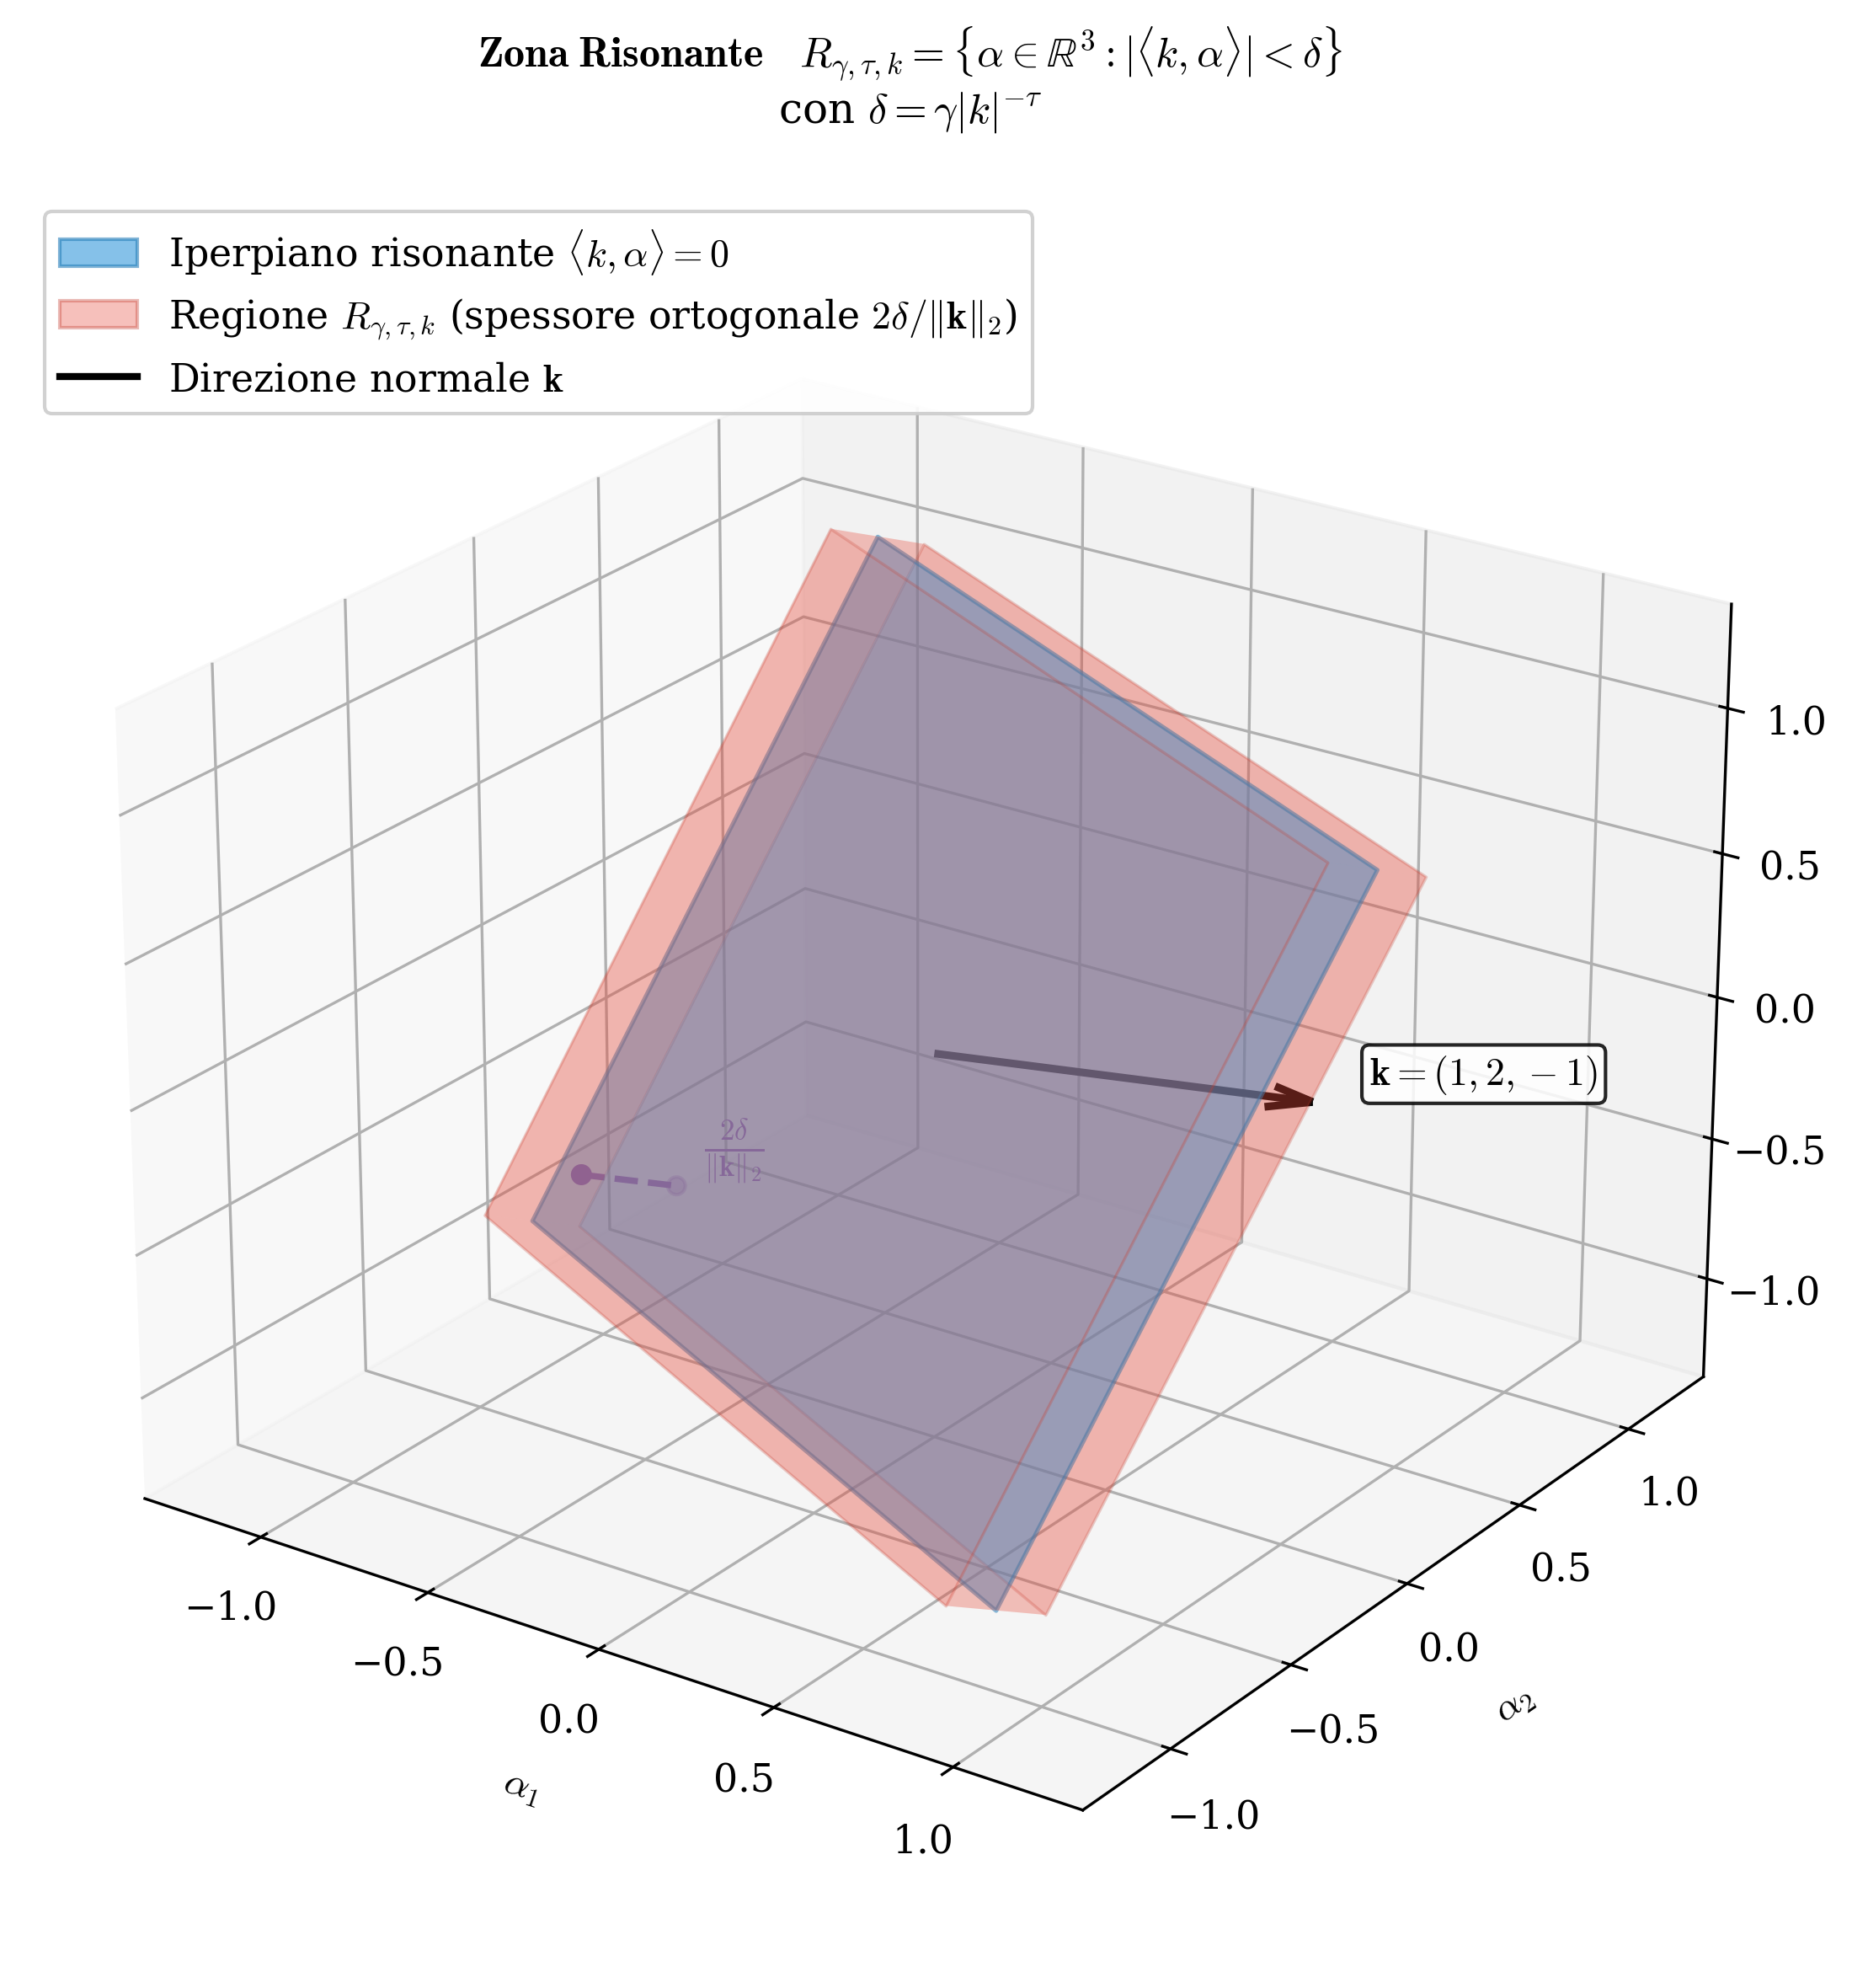
\includegraphics[width=0.75\linewidth]{immagini/r_gamma_tau_k_3d.png}
        \label{fig:placeholder}
        \caption{visualizzazione vettori risontanti in 3D}
    \end{figure}
\end{center}
Considerando l'unione per ogni $k \neq 0$ si ottiene
\begin{align}
    m(R_{\gamma, \tau} \cap \Omega) \leq \sum_{k \neq 0}m(R_{\gamma, \tau, k} \cap \Omega) = O(\gamma)
\end{align}
se $\tau > n - 1$, in modo che la serie converga. Pertanto
\begin{align}
    m(R_\tau) \leq \sum_\gamma m\left(R_{\gamma, \tau}\right) = 0
\end{align}
ovvero $R_\tau$ ha misura di Lebesgue piena in $\mathbb{R}^n$.
\end{proof}
Data una funzione $f$ analitica su un dominio $D \subset \mathbb{C}$, sappiamo, per la \textit{formula integrale di Cauchy}, che 
\begin{align}
    f(z) = \frac{1}{2\pi i}\int_{\mathcal{C}} \frac{f(\omega)}{\omega - z} \, d\omega
\end{align}
dove $\mathcal{C}$ è una circonferenza contenuta in $\mathring{D}$, per ogni $z$ racchiuso dalla circonferenza $\mathcal{C}$. Inoltre, si può dimostrare che differenziando si ottiene
\begin{align}
    f'(z) = \frac{1}{2\pi i}\int_{\mathcal{C}} \frac{f(\omega)}{(\omega - z)^2} \, d\omega
\end{align}
Notiamo che usando la \textit{formula integrale di Cauchy} è possibile determinare $f'$ solamente per i punti interni di $D$, infatti se $z \in \partial D$ non esiste nessuna circonferenza che lo racchiude e che è contenuta interamente in $D$. Segue che
\begin{align}
    |f'|_s \leq \sigma^{-1}|f|_{s + \sigma}
\end{align}
ovvero è possibile al più stimare la norma di $f'$ su un dominio ridotto di $\sigma > 0$, che può però essere arbitrariamente piccolo. \\
In generale, ogni operatore differenziale soddisferà una stima simile.
\begin{prop}[equazione omologica]\label{HomEq&CauchyEst} siano $\alpha \in D_{\gamma, \tau}$ e $s, \sigma > 0$. Se $g \in \mathcal{A}(\mathbb{T}^n_{s + \sigma})$ ha media spaziale nulla esiste unica $f \in \mathcal{A}(\mathbb{T}^n_s)$ con media spaziale nulla tale che $\mathcal{L}_\alpha f = g$. In particolare
\begin{align}
    |f|_s \leq C\gamma^{-1}\sigma^{-n-\tau}|g|_{s + \sigma}
\end{align}
dove $C$ è una costante che dipende solamente dalla dimensionalità dello spazio e da $\tau$. In particolare se $g$ ha media nulla, anche $f$ ha media nulla.
\end{prop}

\begin{proof} consideriamo l'espansione di Fourier di $g$
\begin{align}
    g(\theta) = \sum_{k \in \mathbb{Z}^n\setminus\{0\}} g_k e^{ik \cdot \theta}
\end{align}
Come visto in \eqref{UniqueSol}, l'equazione $\mathcal{L}_\alpha f = g$ ammette come unica soluzione
\begin{align}
    f(\theta) = \sum_{k \in \mathbb{Z}^n\setminus\{0\}} \frac{g_k}{ik \cdot \alpha}e^{ik \cdot \theta}
\end{align}
Per definizione
\begin{align}\label{CoeffEst}
    |g_k| = \left|\int_{\mathbb{T}^n} g(\theta)e^{-ik \cdot \theta} \, d\theta\right|
\end{align}
Per ipotesi $g$ è analitica in $\mathbb{T}^n_{s + \sigma}$, pertanto, per ogni $k \in \mathbb{Z}^n\setminus\{0\}$, trasliamo il toro di integrazione attraverso il diffeomorfismo
\begin{align}
    \theta_j \in \mathbb{T}^n \mapsto \theta_j - i\mathrm{sign}(k_j)(s + \sigma) \in \mathbb{T}^n_{s + \sigma}
\end{align}
per ogni $j = 1, \dots, n$. In particolare \eqref{CoeffEst} viene ora maggiorata da
\begin{align}
    |g_k| \leq |g|_{s + \sigma}e^{-|k|(s + \sigma)}
\end{align}
ovvero i coefficienti di Fourier decadono esponenzialmente (questo è vero per ogni funzione analitica reale). \\
Dato che per ipotesi $\alpha \in D_{\gamma, \tau}$, si ottiene
\begin{align}\label{|f|_s Est}
    |f|_s \leq \frac{|g|_{s + \sigma}}{\gamma}\sum_{k \in \mathbb{Z}^n\setminus\{0\}} |k|^\tau e^{-|k|(s + \sigma)}
\end{align}
Siamo ora interessati a ricondurre la sommatoria ad una sommatoria su $\mathbb{N}$, pertanto, fissato $m \in \mathbb{N}$, dobbiamo contare quanti $k \in \mathbb{Z}^n\setminus\{0\}$ soddisfano $|k| = m$. Notiamo subito che se un dato $k$ soddisfa $|k| = m$, anche $-k$ soddisfa $|-k| = m$, pertanto ottieniamo un fattore $2^n$ a moltiplicare. Ragioniamo quadrante per quadrante, quindi contiamo quanti $k$ nell'insieme
\begin{align}
    \left\{k \in \mathbb{Z}^n\setminus\{0\} : k_i > 0 \text{ per ogni } i = 1, \dots, n\right\}
\end{align}
soddisfano $|k| = m$, fissato $m \in \mathbb{N}$. Se $n = 1$ si ha solamente un elemento, ovvero $k = m$. Se $n = 2$ le soluzioni sono
\begin{align}
    (k_1, k_2) = (m - 1, 1), (m - 2, 2), \dots, (1, m - 1)
\end{align}
che sono $m - 1$. A questi dobbiamo aggiungere i punti
\begin{align}
    (k_1, k_2) = (m, 0), (0, m), (-m, 0), (0, -m)
\end{align}
Pertanto, in totale, si hanno $4(m - 1) + 4 = 4m$ punti. Per $n = 3$, conviene visualizzare il problema, quindi contiamo in quante configurazioni distinte possiamo distribuire $m$ oggetti indistinguibili in $3$ scatole. Equivalentemente possiamo contare quante configurazioni distinte esistono per un insieme composto da $m$ oggetti indistinguibili e $2$ pareti (che separano componenti diverse). Tuttavia, per ragionare su un singolo ottante, dobbiamo escludere gli elementi che hanno almeno una delle componenti nulla, in modo da poter poi moltiplicare per il numero di ottanti ($2^3$) e aggiungere separatamente i termini prima esclusi. Quindi in totale abbiamo
\begin{align}
    8\left(\begin{pmatrix}
        m + 2 \\
        2
    \end{pmatrix} - 3 - 3(m - 1)\right) + 6 + 12(m - 1) &= 4m^2 + 2
\end{align}
Per $n$ arbitrario si ottiene
\begin{align}
    N_n(m) = \sum_{j = 1}^{\min(n, m)} 2^j\begin{pmatrix}
        n \\
        j
    \end{pmatrix} \begin{pmatrix}
        m - 1 \\
        j - 1
    \end{pmatrix}
\end{align}
In particolare, il termine
\begin{align}
    \begin{pmatrix}
        n \\
        j
    \end{pmatrix}
\end{align}
è il numero di modi in cui si possono scegliere $j$ coordinate non nulle (positive), mentre
\begin{align}
    \begin{pmatrix}
        m - 1 \\
        j - 1
    \end{pmatrix}
\end{align}
è il numero di elementi che vivono in un quadrante $j$-dimensionale, si ottiene considerando tutte le configurazione distinte per un insieme di $m - j$ ($-j$ per imporre che nessuna componente sia nulla) oggetti indistinguibili e $j - 1$ pareti. Pertanto \eqref{|f|_s Est} diventa
\begin{align}
    |f|_s \leq \frac{|g|_{s + \sigma}}{\gamma} \sum_{m \in \mathbb{N}}\sum_{j = 1}^{\min(n, m)} 2^j\begin{pmatrix}
        n \\
        j
    \end{pmatrix} \begin{pmatrix}
        m - 1 \\
        j - 1
    \end{pmatrix} m^\tau e^{-m(s + \sigma)}
\end{align}
La somma termina a $\min(n, m)$ perché stiamo considerando $j$ componenti non nulle e imponiamo $|k| = m$. Osserviamo che, fissato $n \in \mathbb{N}$, $N_n(m)$ è un polinomio di grado $n - 1$, infatti
\begin{align}
    \begin{pmatrix}
        m - 1 \\
        j - 1
    \end{pmatrix} = \frac{(m - 1)\cdot \dots \cdot(m - j + 1)}{(j - 1)!}
\end{align}
e il valore massimo che $j$ può assumere è $n$. Pertanto esiste $C_n \in \mathbb{R}$ tale che
\begin{align}
    N_n(m) \leq C_n m^{n - 1}
\end{align}
per ogni $m \in \mathbb{N}$. Quindi possiamo maggiorare $|f|_s$ con
\begin{align}
    |f|_s \leq \frac{C_n |g|_{s + \sigma}}{\gamma}\sum_{m \in \mathbb{N}} m^{\tau + n - 1}e^{-m\sigma}
\end{align}
dove si è maggiorato $e^{-m(s + \sigma)} = e^{-sm}e^{-m\sigma}$ con $e^{-s\sigma}$ dato che $e^{-ms} < 1$ per ogni $s > 0$ e ogni $m \in \mathbb{N}$. \\
A questo punto siamo interessati a maggiorare la sommatoria con un integrale. In particolare si può dimostrare che
\begin{align}
    \sum_{m \in \mathbb{N}} m^{\tau + n - 1}e^{-m\sigma} \leq \int_1^\infty m^{\tau + n - 1}e^{-(m - 1)\sigma} \, dm
\end{align}
Poniamo $t = m\sigma$, allora
\begin{align}
    \int_1^\infty m^{\tau + n - 1}e^{-(m - 1)\sigma} \, dm &= \frac{e^\sigma}{\sigma^{\tau + n}}\int_\sigma^\infty t^{\tau + n - 1}e^{-t} \, dt = \frac{e^\sigma}{\sigma^{\tau + n}}\Gamma(\tau + n)
\end{align}
Ponendo $C_{n, \tau} = e^\sigma\Gamma(\tau + n)C_n$ si ottiene
\begin{align}
    |f|_s \leq C_{n, \tau}\gamma^{-1}\sigma^{-\tau - n}|g|_{s + \sigma}
\end{align}
ovvero la tesi.
\end{proof}
\begin{rmk}
Per definizione di derivata di Lie si ha
\begin{align}
    \mathcal{L}_\alpha f = \left.\frac{d}{dt}\right|_{t = 0} f \circ \varphi_t = \left.\frac{d}{dt}\right|_{t = 0} f(\theta + t\alpha) = f' \cdot \alpha
\end{align}
Inoltre, osserviamo che
\begin{align}
    \frac{d}{dt} f \circ \varphi_t = (f' \circ \varphi_t) \cdot \alpha
\end{align}
Quindi
\begin{align}
    (\mathcal{L}_\alpha f) \circ \varphi_t = \frac{d}{dt} f \circ \varphi_t
\end{align}
Pertanto $\mathcal{L}_\alpha f = g$ diventa
\begin{align}
    \frac{d}{dt} f \circ \varphi_t = g \circ \varphi_t
\end{align}
A questo punto possiamo integrare entrambi i membri lungo $(0, \tau)$, $\tau > 0$, ottenendo
\begin{align}
    f \circ \varphi_\tau - f = \int_0^\tau g \circ \varphi_t \, dt
\end{align}
o equivalentemente
\begin{align}
    \frac{f \circ \varphi_\tau (\theta) - f(\theta)}{\tau} = \frac{1}{\tau}\int_0^\tau g \circ \varphi_t(\theta) \, dt
\end{align}
per ogni $\theta \in \mathbb{T}^n$. \\
Dato che cerchiamo una soluzione $f$ regolare su $\mathbb{T}^n$, che è compatto, deve necessariamente essere anche limitata. Pertanto, al limite $\tau \rightarrow \infty$, il membro di sinistra deve annullarsi, mentre il membro di destra, per ergodicità del flusso lineare $\varphi_t$, può essere sostituito con la media spaziale di $g \circ \varphi_t$ per la proposizione \ref{NonResErgFlowEq}, che equivale alla media spaziale di $g$ per invarianza di $\mathbb{T}^n$ rispetto a $\varphi_t$. Si ottiene quindi la condizione di media spaziale nulla per $g$. \\ \\
Inoltre, sempre per la proposizione \ref{NonResErgFlowEq}, sappiamo che le uniche funzioni invarianti per flusso sono le funzioni costanti, segue che $\mathcal{L}_\alpha f = 0$ se e solo se $f$ è costante su $\mathbb{T}^n$. Pertanto, una volta fissata la condizione
\begin{align}
    \overline{f} = \int_{\mathbb{T}^n} f(\theta) \, d\theta = 0
\end{align}
si ottiene automaticamente l'unicità della soluzione $f$, per iniettiva dell'operatore lineare $\mathcal{L}_\alpha$ sul sottoinsieme delle funzioni non costanti.
\end{rmk}
Come visto in \ref{HomEq&CauchyEst}, la risoluzione dell'equazione omologica comporta una perdita di analiticità $\sigma > 0$, arbitrariamente piccola. \\ \\
Per dimostrare il teorema di Herman (\ref{TwistThmHerman2}) dovremo risolvere un'equazione non lineare, che però è di natura perturbativa, pertanto avrà senso applicare al problema uno schema alla Newton, ovvero risolvere iterativamente l'equazione linearizzata nel punto fornito dall'equazione linearizzata precedente, costruendo così una successione di punti che convergerà alla soluzione. \\ \\
Ogni passo dello schema alla Newton prevederà la risoluzione di equazioni omologiche, che causaranno la caratteristica perdita di analitica. \\
Tuttavia, come prima accennato, la perdita di analiticità può essere abritrariamente piccola, pertanto potremo scegliere di perdere ad ogni passo una quantità controllata di analiticità $\sigma_k > 0$, in modo tale che la somma delle quantità perse $\sum \sigma_k$ converga ad un valore finito e ci permetta quindi di avere ancora un dominio di analiticità di estensione finita al termine dell'algoritmo risolutivo. \\
Inoltre, la superconvergenza del metodo iterativo alla Newton schiaccia nettamente la stime di Cauchy sulle soluzioni delle equazioni omologiche, che saranno sempre più deboli a causa della scelta fatta sulla successione $(\sigma_k)_k$.

\chapter{Persistenza di tori invarianti quasi-periodici}
Ora vogliamo determinare se il toro invariante $\alpha$-quasi-periodico $T^n_0$ persiste, seppur leggermente deformato, per piccole perturbazioni del sistema integrabile. \\
A tal proposito vogliamo trovare un simplettomorfismo $G$ che coniughi il sistema integrabile e la perturbazione.
\section{Il teorema \textit{twist} di Herman}
Consideriamo lo spazio $\mathcal{H}$ dei germi lungo $T^n_0 = \mathbb{T}^n \times \{0\}$ delle hamiltoniane analitiche reali. Sia $\mathcal{K}^\alpha$ il sottospazio affine dell'hamiltoniane analitiche reali della forma
\begin{align}
    K(\theta, r) = c + \alpha \cdot r + O(r^2) 
\end{align}
con $c \in \mathbb{R}$ e $\alpha \in \mathbb{R}^n$, dove con $O(r^2)$ intendiamo un termine di resto $P = P(\theta, r)$ che soddisfa
\begin{align}
    \begin{cases}
        P(\theta, 0) = 0 \\
        \frac{\partial P}{\partial r}(\theta, 0) = 0
    \end{cases}
\end{align}
per ogni $\theta \in \mathbb{T}^n$. Tali hamiltoniane soddisfano
\begin{align}\label{HamVectFieldK}
    X_K|_{T^n_0} = \begin{pmatrix}
        \alpha \\
        0
    \end{pmatrix} 
\end{align}
ovvero $T^n_0$ è un toro invariante quasi-periodico di frequenza $\alpha$ per il flusso associato a $X_K$. \\
Infine sia $\mathcal{G}$ lo spazio dei germi lungo $T^n_0$ dei simplettomorfismi esatti della forma
\begin{align}\label{ExactSympl}
    G(\theta, r) = (\varphi(\theta), \null^t\varphi'(\theta)^{-1}(r + \rho(\theta)))
\end{align}
dove $\varphi$ è isomorfismo del toro $\mathbb{T}^n$ che fissa l'origine, mentre $\rho$ è una $1$-forma esatta su $\mathbb{T}^n$, ovvero è il differenziale di una funzione reale liscia $S$ su $\mathbb{T}^n$
\begin{align}
    \rho = dS \qquad S : \mathbb{T}^n \longrightarrow \mathbb{R}
\end{align}
Ricordiamo la notazione per lo spazio delle fasi
\begin{align}
    \mathbb{T}^n = \mathbb{R}^n/2\pi\mathbb{Z}^n \qquad T^n_0 := \mathbb{T}^n \times \{0\} \subset \mathbb{T}^n \times \mathbb{R}^n
\end{align}
le estensioni complesse
\begin{align}
    \mathbb{T}^n_\mathbb{C} = \mathbb{C}^n/2\pi\mathbb{Z}^n \qquad T^n_{\mathbb{C}} := \mathbb{T}^n_\mathbb{C} \times \mathbb{C}^n
\end{align}
e gli intorni
\begin{align}
    \mathbb{T}^n_s &:= \{\theta \in \mathbb{T}^n_\mathbb{C} : \max_j |\mathrm{Im} \, \theta_j| \leq s\} \\
    T^n_s &:= \{ (\theta, r) \in T^n_\mathbb{C} : \max_j \max(|\mathrm{Im} \, \theta_j|, |r_j|) \leq s\}
\end{align}
\begin{thm}[\textit{twist} di Herman, cfr. \cite{Massetti}]\label{TwistThmHerman1} dati $\alpha \in D_{\gamma, \tau}$ e $K^0 \in \mathcal{K}$, per ogni $H \in \mathcal{H}$ sufficientemente vicina a $K^0$ esiste unico $(K, G, \beta) \in \mathcal{K} \times \mathcal{G} \times \mathbb{R}^n$ vicina a $(K^0, \mathrm{id}, 0)$ tale che
\begin{align}\label{TwistNormalForm}
    H - \beta \cdot r = K \circ G 
\end{align}
in un intorno di $T^n_0$.
\end{thm}
Essendo il vettore frequenza invariante per coniugazioni topologiche, dato che $G$ è un simplettomorfismo, il termine $\beta \cdot r$ diventa necessario, tuttavia, rompe la coniugazione dinamica tra $K$ e $H$. \\
Notiamo che non avrebbe senso sperare di ottenere un'identità della forma
\begin{align}
    H = (K + \beta \cdot r) \circ G
\end{align}
Infatti, ciò comporterebbe che possedere un toro invariante quasi-periodico sia una proprietà aperta, ovvero che per ogni $K \in \mathcal{K}^\alpha$ sia possibile trovare un intorno aperto sufficientemente piccolo tale che ogni elemento di tale intorno possieda un toro invariante quasi periodico, quindi che sia una proprietà stabile per piccole perturbazioni di $K$. \\
Infatti, possiamo costruire un esempio di funzione analitica reale $H$ arbitariamente vicina a $K$ che non ammette un toro invariante quasi-periodico. A tal proposito consideriamo $K$ della forma
\begin{align}
    K = \alpha \cdot r
\end{align}
A meno di aggiungere una prima perturbazione arbitraria, possiamo supporre che $\alpha$ sia risonante, ovvero che esiste $k \in \mathbb{Z}^n$ tale che $k \cdot \alpha = 0$ (densità dei vettori non diofantei in $\mathbb{R}^n$). Pertanto aggiungiamo a $K$ un termine risonante, dipendente da $\theta$ in modo periodico e proporzionale ad un parametro $\varepsilon > 0$ arbitrario e definiamo
\begin{align}
    H = K - \varepsilon\sin(k \cdot \theta) = \alpha \cdot r - \varepsilon\sin(k \cdot \theta)
\end{align}
Il campo vettoriale hamiltoniano $X_H$ associato a $H$ è
\begin{align}
    X_H = \begin{pmatrix}
        \alpha \\
        \varepsilon k\cos(k \cdot \theta)
    \end{pmatrix}
\end{align}
Pertanto la restrizione del flusso hamiltoniano a $\{0\} \times \mathbb{R}^n$ fornisce
\begin{align}
    \varphi_t : (0, r) \mapsto (t\alpha, t\varepsilon k)
\end{align}
quindi è non limitato per $\varepsilon > 0$.
\begin{rmk} consideriamo l'hamiltoniana $\widehat{H} := H - \beta \cdot r = K \circ G$. \\
$\mathbb{T}^n \times \{0\}$ è invariante per il flusso di $X_K$, come visto in \eqref{HamVectFieldK}. Inoltre, $K|_{\mathbb{T}^n \times \{0\}} = c$ costante, quindi
\begin{align}
    \widehat{H} := H - \beta \cdot r = K \circ G
\end{align}
è costante su $G^{-1}(\mathbb{T}^n \times \{0\}) = Gr \, (-\rho)$ varietà lagrangiana (grafico della $1$-forma chiusa $-\rho$). Pertanto $G^{-1}(\mathbb{T}^n \times \{0\})$ è invariante per il flusso hamiltoniano associato a $X_{\widehat{H}}$, per il lemma \ref{LemBost}.
\end{rmk}
Una volta dimostrato il risultato del \cref{TwistThmHerman1}, mostreremo che il controtermine $\beta$ può essere eliminato, sotto opportune ipotesi di non degenerazione.
\subsection{Setting funzionale}\label{SettingFunz}
Impostiamo gli spazi funzionali necessari per introdurre e lavorare con l'operatore
\begin{align}
    \phi : (K, G, \beta) \mapsto H = K \circ G + \beta \cdot r 
\end{align}
in modo da provare il \textit{teorema twist di Herman} come conseguenza del fatto che $\phi$ è un diffeomorfismo locale attorno a $(K^0, \mathrm{id}, 0)$, per $\alpha$ $(\gamma, \tau)$-diofanteo. \\ \\
Sia $\mathcal{H}_s = (\mathcal{A}(T^n_s), |\cdot|_s)$, dove
\begin{align}
    |H|_s = \sup_{(\theta, r) \in T^n_s} |H(\theta, r)| 
\end{align}
in modo tale che sia uno spazio di Banach. \\
Dato $\alpha \in \mathbb{R}^n$ poniamo $\mathcal{K}_s := \mathcal{K}^\alpha_s$ lo spazio affine composto dai $K \in \mathcal{H}_s$ tali che
\begin{align}
    K = c + \alpha \cdot r + O(r^2) 
\end{align}
per qualche $c \in \mathbb{R}$. \\
Dato $G$ isomorfismo analitico reale definito su un aperto di $T^n_{\mathbb{C}}$, poniamo
\begin{align}
    G^*\mathcal{A}(T^n_s) = \mathcal{A}(G^{-1}(T^n_s)) \notag
\end{align}
e vi definiamo la norma
\begin{align}
    |H|_{G, s} = |H \circ G^{-1}|_s 
\end{align}
Così facendo, $|\cdot|_{G, s}$ rende $\mathcal{H}_{s - |G - \mathrm{id}|_s}$ uno spazio di Banach. In particolare si ha che
\begin{align}
    G^* : H \in \mathcal{A}(T^n_s) \mapsto G^*H = H \circ G \in \mathcal{A}(G^{-1}(T^n_s)) 
\end{align}
è un isometria suriettiva, infatti
\begin{align}
    |G^*H|_{G, s} = |H \circ G|_{G, s} = |H \circ G \circ G^{-1}|_s = |H|_s
\end{align}
e, dato che $G$ è un isomorfismo, data $\widetilde{H} \in G^*\mathcal{A}(T^n_s)$, si ha che $G_*\widetilde{H} = \widetilde{H} \circ G^{-1}$ è un elemento di $\mathcal{A}(T^n_s)$ che soddisfa
\begin{align}
    G^*(G_*\widetilde{H}) = G^*(\widetilde{H} \circ G^{-1}) = (\widetilde{H} \circ G^{-1}) \circ G = \widetilde{H}
\end{align}
Gli isomorfismi suriettivi preservano la completezza, quindi anche $G^*\mathcal{A}(T^n_s)$ è uno spazio di Banach. \\
La perdita di $|G - \mathrm{id}|_s$ nell'estensione del dominio di analiticità è dovuta al fatto che $G$ deforma $T^n_s$, pertanto è necessario restringere il dominio di $\sigma > |G - \mathrm{id}|_s$ in modo tale da ottenere $G(T^n_{s - \sigma}) \subset T^n_s$. Così facendo, ad ogni passo lavoreremo con funzioni analitiche su insiemi del tipo $T^n_{s - \sigma_k}$, inoltre sarà valida la maggiorazione naturale
\begin{align}
    |G^*H|_{s - \sigma} \leq |H|_s
\end{align}
Sia $\mathcal{D}_s$ lo spazio degli isomorfismi analitici reali $\varphi : \mathbb{T}^n_s \longrightarrow \varphi(\mathbb{T}^n_s)$ che fissano l'origine. \\
Inoltre, sia $\chi_s$ lo spazio dei campi vettoriali su $\mathbb{T}^n_s$ nulli all'origine, con norma
\begin{align}
    |v|_s = \max_j \sup_{\theta \in \mathbb{T}^n_s} |v_j(\theta)|
\end{align}
che lo rende uno spazio di Banach. \\
Vogliamo fornire a un intorno dell'identità in $\mathcal{D}_s$ struttura di varietà di Banach, in modo da poter definire uno spazio tangente e derivare in senso di Fréchet (cfr. \ref{FrechDervDefn}). In particolare si può dimostrare che la mappa
\begin{align}
    v \mapsto \mathrm{id} + v
\end{align}
definita dall'aperto
\begin{align}
    \sigma\mathring{B}^\chi_{s + \sigma} = \{v \in \chi_{s + \sigma} : |v|_s < \sigma\}
\end{align}
a $\mathcal{D}_s$ è biettiva (cfr. \cite{Fejoz17}), pertanto fornisce a $\mathcal{D}_s$ struttura di varietà di Banach in un intorno dell'identità. \\ \\
Siamo interessati in particolare all'azione controgradiente degli elementi di $\mathcal{D}_s$ su $T^n_s$, come visto in \eqref{ContraGrad}, che ci permetterà di linearizzare la dinamica sul toro invariante. \\ \\
Inoltre, consideriamo lo spazio $\mathcal{B}_s$ delle $1$-forme differenziali esatte su $\mathbb{T}^n_s$ del tipo
\begin{align}
    \rho : (\theta, r) \mapsto (\theta, r + \rho(\theta)) \qquad \rho_0 = 0
\end{align}
ovvero che agiscono per traslazione delle azioni, in modo da raddrizzare il toro invariante perturbato. Su $\mathcal{B}_s$ definiamo la norma
\begin{align}
    |\rho|_s = \max_j \sup_{\theta \in \mathbb{T}^n_s} |\rho_j(\theta)|
\end{align}
Identifichiamo con $\mathcal{G}_s = \mathcal{D}_s \times \mathcal{B}_s$ lo spazio dei simplettomorfismi del tipo
\begin{align}
    G = (\varphi, \rho) : (\theta, r) \mapsto (\varphi(\theta), \null^t\varphi'(\theta)^{-1}(r + \rho(\theta)))
\end{align}
Definiamo su $T_{\mathrm{id}}\mathcal{G}_s = \mathfrak{g}_s = \chi_s \times \mathcal{B}_s$ la norma
\begin{align}
    |\dot{G}|_s = |(\dot{v}, \dot{\rho})|_s = \max(|\dot{v}|_s, |\dot{\rho}|_s) \qquad (\dot{v}, \dot{\rho}) \in \mathfrak{g}_s
\end{align}
Mentre su $T_G\mathcal{G}_s$ la norma
\begin{align}
    |\delta G|_{G, s} = |\delta G \circ G^{-1}|_s \qquad \delta G \in T_G\mathcal{G}_s
\end{align}
Come accade per le varietà classiche, anche per varietà di Banach lo spazio tangente ad un punto può essere identificato con lo spazio di Banach modello (tramite isomorfismi), pertanto, in questo contesto, $\dot{G}$ e $\delta G$ non sono altro che elementi di $\chi_s \times \mathcal{B}_s$. Segue che $\delta G \circ G^{-1}$ è un elemento dello spazio tangente all'identità. \\ \\
Infine, consideriamo l'intorno dell'identità
\begin{align}
    \mathcal{G}^\sigma_s = \{G \in \mathcal{G}_s : \sup_{(\theta, r) \in T^n_s} |(\Theta - \theta, R - r)| < \sigma, (\Theta, R) = G(\theta, r), \sigma > 0\}
\end{align}
i cui elementi sono tutti i simplettomorfismi in $\mathcal{G}_s$ che sono al più $\sigma$-lontani dall'identità, come prima discusso. \\ \\
A questo punto è ben definito l'operatore
\begin{align}
    \phi : (K, G, \beta) \in \mathcal{K}_{s + \sigma} \times \mathcal{G}^\sigma_{s + \sigma} \times \mathbb{R}^n \mapsto H = K \circ G + \beta \cdot r \in \mathcal{H}_s
\end{align}
Inoltre, posto $E_s = \mathcal{K}_s \times \mathcal{G}_s \times \mathbb{R}^n$ e il suo aperto
\begin{align}
    \sigma B^E_s = \{x \in E_s : |x|_s < \sigma\}
\end{align}
è ben definita la restrizione
\begin{align}
    \phi : \sigma B^E_{s + \sigma} \longrightarrow \mathcal{H}_s
\end{align}
a cui applicheremo il \textit{teorema della funzione inversa} \ref{InvFunctThm}. \\ \\
A questo punto possiamo riformulare il \textit{teorema di Herman} \ref{TwistThmHerman1} in termini dell'operatore $\phi$ e della sua inversa locale $\psi$.
\begin{thm}[\textit{twist} di Herman, cfr. \cite{Fejoz17}]\label{TwistThmHerman2} sia $\alpha \in D_{\gamma, \tau}$, l'operatore $\phi$ ammette inversa locale unica $\psi$ nel senso che per ogni $0 < s < s + \sigma < 1$, data $K^0 \in \mathcal{K}_{s + \sigma}$, se $|H - K^0|_{s + \sigma}$ è sufficientemente piccolo, esiste unica $(K, G, \beta) \in \sigma B^E_s$, $|\cdot|_s$-vicina a $(K^0, \mathrm{id}, 0)$, tale che
\begin{align}
    \psi(H) = (K, G, \beta) \qquad H = K \circ G + \beta \cdot r
\end{align}
su $T^n_s$. Inoltre, $\beta \circ \psi$ è di classe $C^1$ in un $|\cdot|_{s + \sigma}$-intorno di $K^0$.
\end{thm}
\subsection{Invertibilità di $\phi'$ e stime su $\phi'^{-1}$ e $\phi''$}
Verifichiamo che $\phi$ soddisfa le condizioni necessarie per applicare lo schemo iterativo alla Newton con perdita controllata di analiticità alla Nash-Moser. \\
Poniamo $x = (K, G, \beta)$ e $\delta x = (\delta K, \delta G, \delta \beta)$ e fissiamo $0 < s < s + \sigma < 1$.
\begin{lemma} esiste $C' > 0$ localmente uniforme rispetto a $x \in E_{s + \sigma}$ in un intorno di $G = \mathrm{id}$ tale che la mappa $\phi'(x)$ ammette inversa locale $\phi'(x)^{-1}$ che soddisfa
\begin{align}
    |\phi'(x)^{-1}\delta H|_{s} \leq C'\sigma^{-\tau - n - 1}|\delta H|_{G, s + \sigma}
\end{align}
\end{lemma}

\begin{proof} prima di tutto determiniamo la mappa lineare $\phi'(x)$ che soddisfa
\begin{align}
    \lim_{|\delta x|_{s + \sigma} \rightarrow 0} \frac{|\phi(x + \delta x) - \phi(x) - \phi'(x)\delta x|_{G, s}}{|\delta x|_{s + \sigma}} = 0
\end{align}
A tal proposito individuiamo tutti i termini lineari in $\delta x$ presenti nel rapporto incrementale e li annulliamo, incorporandoli in $\phi'(x)\delta x$. In particolare
\begin{align}
    \phi(x + \delta x) &= (K + \delta K) \circ (G + \delta G) + (\beta + \delta \beta) \cdot r \notag \\
    &= K \circ (G + \delta G) + \delta K \circ (G + \delta G) + (\beta + \delta \beta) \cdot r
\end{align}
Pertanto
\begin{align}
    \phi(x + \delta x) - \phi(x) &= K \circ (G + \delta G) + \delta K \circ (G + \delta G) + \delta\beta \cdot r - K \circ G
\end{align}
Prendendo la norma $|\cdot|_{G, s}$ si ottiene
\begin{gather}
    |\phi(x + \delta x) - \phi(x) - \phi'(x)\delta x|_{G, s} = \notag \\
    = |((K + \delta K )\circ (G + \delta G) - K \circ G + (\delta\beta \cdot r) - \phi'(x)\delta x) \circ G^{-1}|_{s} \notag \\
    = |(K \circ (G + \delta G) - K \circ G + \delta K \circ (G + \delta G) + (\delta\beta \cdot r) - \phi'(x)\delta x)\circ G^{-1}|_s
\end{gather}
Quindi
\begin{align}
    \phi'(x)\delta x = (K' \circ G)\delta G + \delta K \circ G + \delta\beta \cdot r 
\end{align}
dove il termine $(K' \circ G)\delta G$ deriva dal rapporto incrementale
\begin{align}
    \frac{|K \circ (G + \delta G) - K \circ G|_{G, s}}{|\delta x|_{s + \sigma}} = \frac{|K(G + \delta G) - K(G)|_{G, s}}{|\delta x|_{s + \sigma}}
\end{align}
che, per definizione, al limite fornisce $K'(G) = K' \circ G$, dato che $|\delta G|_{s + \sigma} \leq |\delta x|_{s + \sigma}$. Il termine $\delta K \circ G$ rimane perché è lineare in $\delta K$, infatti
\begin{align}
    \delta K \circ (G + \delta G) = \delta K \circ G + R
\end{align}
dove $|R|_{G, s} = o(|\delta x|_{s + \sigma})$. Analogamente, sopravvive anche il termine $\delta\beta \cdot r$, lineare in $\delta\beta$. \\
A questo punto, dato $\delta H \in G^*\mathcal{A}(T^n_s)$, vogliamo risolvere
\begin{align}
    \phi'(x)\delta x = (K' \circ G)\delta G + \delta K \circ G + \delta\beta \cdot r = \delta H
\end{align}
o, componendo a destra con $G^{-1}$, risolvere
\begin{align}\label{LinEqDphi}
    K' \cdot \dot{G} + \delta K + (\delta\beta \cdot r) \circ G^{-1} = \dot{H}
\end{align}
dove $\dot{H} \in \mathcal{H}_{s + \sigma}$. In particolare, dato che $K \in \mathcal{K}_{s + \sigma}$ è della forma
\begin{align}
    K = c + \alpha \cdot r + O(r^2)
\end{align}
con $c \in \mathbb{R}$ e $\alpha \in D_{\gamma, \tau}$ fissato, possiamo scrivere $\delta K = \delta c + O(r^2)$, quindi
\begin{align}
    K' \cdot \dot{G} + \delta c + (\delta\beta \cdot r) \circ G^{-1} + O(r^2) = \dot{H}
\end{align}
In particolare risolvendo
\begin{align}
    \begin{cases}
        \Theta &= \varphi(\theta) \\
        R &= \null^t\varphi'(\theta)^{-1}(r + \rho(\theta))
    \end{cases}
\end{align}
si ottiene
\begin{align}
    \begin{cases}
        \theta &= \varphi^{-1}(\Theta) \\
        r &= \null^t\varphi'(\theta)R - \rho(\theta)
    \end{cases}
\end{align}
Pertanto, a meno di rinominare $(\Theta, R)$ in $(\theta, r)$, si ottiene
\begin{align}
    G^{-1} : (\theta, r) \mapsto (\varphi^{-1}(\theta), \null^t\varphi' \circ \varphi^{-1} \, (\theta)r - \rho \circ \varphi^{-1} \, (\theta))
\end{align}
Osserviamo che
\begin{align}\label{DeltaG}
    \delta G = (\delta \varphi, \delta((r + \rho)\varphi'^{-1}))
\end{align}
Inoltre, $\delta(\varphi'^{-1}\varphi') = 0$, pertanto otteniamo
\begin{align}
    \delta\varphi'^{-1}\varphi' + \varphi'^{-1}\delta\varphi' = 0
\end{align}
ovvero
\begin{align}
    \delta\varphi'^{-1} = -\varphi'^{-1}\delta\varphi'\varphi'^{-1}
\end{align}
Sostituendo in \eqref{DeltaG}, si ottiene
\begin{align}
    \delta G = (\delta\varphi, \delta\rho \, \varphi'^{-1} - (r + \rho)\varphi'^{-1}\delta\varphi'\varphi'^{-1})
\end{align}
Quindi, pre-componendo per $G^{-1}$, si ha
\begin{align}
    \delta G \circ G^{-1} = (\delta \varphi \circ \varphi^{-1}, \delta\rho \, \varphi'^{-1} - r\delta\varphi'\varphi'^{-1})
\end{align}
In particolare, $\delta\varphi \circ \varphi^{-1}$ è un vettore tangente all'identità in $\mathcal{D}_s$, pertanto è della forma $\dot{\varphi}$, e, analogamente, $\delta\varphi'\varphi'^{-1}$ è della forma $\dot{\varphi}'$. Infine, ponendo $\dot{\rho} = \delta \rho \, \varphi'^{-1}$, si ottiene
\begin{align}
    \delta G \circ G^{-1} = (\dot{\varphi}, \dot{\rho} - r\dot{\varphi}')
\end{align}
Sviluppando
\begin{align}
    K &= c + \alpha \cdot r + K_2(\theta)r \cdot r + O(r^3) \\
    \dot{H} &= \dot{H}_0(\theta) + \dot{H}_1(\theta) \cdot r + O(r^2)
\end{align}
\eqref{LinEqDphi} diventa
\begin{gather}
    (\delta c - \alpha \cdot \dot{\rho} - \rho \circ \varphi^{-1} \, (\theta) \cdot \delta\beta) \ + \notag \\
    \label{HomEqs}
    + \ r \cdot (\dot{\varphi}' \cdot \alpha + \varphi' \circ \varphi^{-1} \, (\theta) \cdot \delta\beta - 2K_2(\theta)\dot{\rho}) = \dot{H} + O(r^2)
\end{gather}
dove si è usato
\begin{align}
    K' = \begin{pmatrix}
        O(r^2) \\
        \alpha + 2K_2(\theta)r + O(r^2)
    \end{pmatrix}
\end{align}
In particolare i termini $O(r^2)$ in \eqref{HomEqs} dipendono esclusivamente da $K$ e da $\dot{G}$. \\ 
A questo punto (applicando \cite[Proposizione~24]{Fejoz02} per garantire che $\delta\beta$ sia ben definito), posti
\begin{align}
    \delta\beta &= \left(\int_{\mathbb{T}^n} \varphi' \circ \varphi^{-1} \, d\theta\right)^{-1}\int_{\mathbb{T}^n} \dot{H}_1 \, d\theta \\
    \delta c &= \int_{\mathbb{T}^n} \dot{H}_0 \, d\theta + \int_{\mathbb{T}^n} \rho \circ \varphi^{-1} \, d\theta \cdot \delta\beta
\end{align}
\eqref{HomEqs} diventa
\begin{align}
    -\alpha \cdot \dot{\rho} + r \cdot (\dot{\varphi}' \cdot \alpha - 2K_2(\theta)\dot{\rho}) = \dot{H} + O(r^2)
\end{align}
dove restano solamente i termini di deviazione dalla media dallo sviluppo di $\dot{H}$ (per come abbiamo definito $\delta\beta$ e $\delta c$). \\
A questo punto ricordiamo che $\dot{\rho}$ è, per definizione, una $1$-forma esatta, pertanto può essere scritta come il differenziale di una funzione liscia $f$ su $\mathbb{T}^n$, ovvero possiamo scrivere $-\dot{\rho} = f'$. Pertanto il termine $-\alpha \cdot \dot{\rho}$ diventa esattamente la derivata di Lie lungo il campo costante $\alpha$ della funzione $f$, cioè
\begin{align}\label{HomEqRho}
    -\alpha \cdot \dot{\rho} = \mathcal{L}_\alpha f
\end{align}
Per la proposizione \ref{HomEq&CauchyEst}, \eqref{HomEqRho} ammette un'unica soluzione $f$ che risolve l'equazione omologica e soddisfa
\begin{align}
    |f|_{s + \sigma} \leq A\gamma^{-1}\sigma^{-\tau - n}|\widetilde{\dot{H}}_0|_s
\end{align}
dove si è chiamato $\widetilde{\dot{H}}_0$ la deviazione di $\dot{H}_0$ dalla sua media spaziale, per qualche $A > 0$. Segue che
\begin{align}
    |\dot{\rho}|_s \leq A'\gamma^{-1}\sigma^{-\tau - n - 1}|\widetilde{\dot{H}}_0|_s
\end{align}
per qualche $A' > 0$. Inoltre, osserviamo che la soluzione all'equazione omologica per $\dot{\rho}$ avrà media nulla. \\
Una volta determinato $\dot{\rho}$ possiamo determinare anche $\dot{\varphi}'$. In particolare, sempre per \eqref{HomEq&CauchyEst}, esiste unico $\dot{\varphi}$ che risolve l'equazione omologica
\begin{align}
    \mathcal{L}_\alpha\dot{\varphi} = \alpha \cdot \dot{\varphi}' = 2K_2(\theta)\dot{\rho} + \dot{H}_1(\theta) - \int_{\mathbb{T}^n} \dot{H}_1(\theta) \, d\theta
\end{align}
e che soddisfa una stima analoga a quella per $\dot{\rho}$. Infine, i termini $O(r^2)$ di $\dot{H}$ determinano i termini $O(r^2)$ di $\delta K$, pertanto, ricordando che $\dot{H} = \delta H \circ G^{-1}$ e quindi che $|\dot{H}|_s = |\delta H|_{G, s}$, si ottiene la tesi.
\end{proof}
\begin{lemma}[cfr. \cite{Massetti}] esiste $C'' > 0$ localmente uniforme rispetto a $x \in E_{s + \sigma}$ in un intorno di $G = \mathrm{id}$ tale che la mappa bilineare $\phi''(x)$ soddisfa
\begin{align}
    |\phi''(x)\delta x^{\otimes 2}|_{G, s} \leq \sigma^{-2}C''|\delta x|^2_{s + \sigma}
\end{align}
\end{lemma}

\begin{proof} determiniamo $\phi''(x)$
\begin{align}
    \phi'(x + \delta x) - \phi'(x) &= ((K + \delta K)' \circ (G + \delta G)) + \circ (G + \delta G) \ + \notag \\
    &- \ (K' \circ G) - \circ \, G \notag \\
    &= (K' \circ (G + \delta G)) - (K' \circ G) \ + \notag \\
    &+ \ \circ (G + \delta G) - \circ \, G \ + \delta K ' \circ (G + \delta G)
\end{align}
Annullando i termini lineari in $\delta x$ si ottiene
\begin{align}
    \phi''(x)\delta x^{\otimes 2} = (K'' \circ G)\delta G^{\otimes 2} + 2(\delta K' \circ G)\delta G
\end{align}
Pertanto
\begin{align}
    \phi''(x)\delta x^{\otimes 2} \circ G^{-1} = 2\delta K' \cdot \dot{G} + K'' \cdot \dot{G}^{\otimes 2}
\end{align}
La tesi segue immediatamente dalla stima di Cauchy, dalla stima sulla norma di composizione $|\cdot|_{G, s}$ e notando che $|\delta K' \cdot \dot{G}|_s \leq |K' \cdot \dot{G}|_s$.
\end{proof}
\begin{proof}[Dimostrazione del teorema di Herman \ref{TwistThmHerman2}]
Il contesto è quello dell'appendice D. Dato $H \in \mathcal{H}_{s + \sigma}$ tale che $|H - K^0|_{s + \sigma} < \epsilon$, per il teorema \eqref{InvFunctThm} e le proposizioni \eqref{LipschCont} e \eqref{PsiC^1}, $\phi$ ammette inversa locale $\psi : \epsilon B^\mathcal{H}_{s + \sigma} \longrightarrow \eta B^{E}_s$ di classe $C^1$ tale che $\psi(H) = K \circ G + \beta \cdot r$.
\end{proof}

\section{Il teorema di Kolmogorov}
\begin{thm}[dei tori invarianti di Kolmogorov, forte non degenerazione]\label{KolmThmStrongNonDeg} siano $\alpha \in D_{\gamma, \tau}$ e $K^0 \in \mathcal{K}$ tale che
\begin{align}
    \det \int_{\mathbb{T}^n} \frac{\partial^2 K^0}{\partial r^2}(\theta, 0) \, d\theta \neq 0 
\end{align}
Per ogni $H \in \mathcal{H}$ vicino a $K^0$ esiste unico $(K, G, R) \in \mathcal{K} \times \mathcal{G} \times \mathbb{R}^n$ vicino a $(K^0, \mathrm{id}, 0)$ tale che
\begin{align}
    H(\theta, r + R) = K \circ G \, (\theta, r) 
\end{align}
in un intorno di $T^n_0$ (che è localmente uniforme rispetto a $H$), quindi $H$ possiede un toro invariante $\alpha$-quasi-periodico.
\end{thm}

\begin{proof} poniamo
\begin{align}
    K^0_2(\theta, 0) := \frac{1}{2}\frac{\partial^2 K^0}{\partial r^2}(\theta, 0) 
\end{align}
Allora possiamo scrivere
\begin{align}\label{SecOrdExpK0}
    K^0 = c + \alpha \cdot r + K^0_2 \cdot r^2 + O(r^3) 
\end{align}
In generale $K^0_2$ non è costante su $T^n_0$, vogliamo quindi cercare un cambio di coordinate simplettico $\varphi$ che ci permetta di avere anche il termine quadratico in $r$ costante rispetto a $\theta$. \\
Per la \ref{HomEq&CauchyEst}, esiste unica $F$ che soddisfa
\begin{align}
    \mathcal{L}_\alpha F(\theta) = \frac{1}{2}\frac{\partial^2 K^0}{\partial r^2}(\theta, 0) - \int_{\mathbb{T}^n} \frac{1}{2}\frac{\partial^2 K^0}{\partial r^2}(\theta, 0) \, d\theta 
\end{align}
Inoltre $F$ ha media nulla su $T^n_0$. Consideriamo l'hamiltoniana ausiliaria $S = F(\theta)r \cdot r$, il campo vettoriale associato è
\begin{align}
    X_S = \left(2F(\theta)r,-\frac{\partial F}{\partial \theta}r \cdot r\right) 
\end{align}
Notiamo che $X_S|_{T^n_0} = (0, 0)$, quindi $\varphi|_{T^n_0} = \mathrm{id}$. In particolare $\varphi$ è determinato da
\begin{align}
    \begin{cases}
        \frac{d\Theta}{dt} &= 2F(\Theta)R \\
        \frac{dR}{dt} &= -\frac{\partial F}{\partial \theta}(\Theta)R \cdot R
    \end{cases} 
\end{align}
Quindi
\begin{align}\label{Time1AusFlow}
    \begin{cases}
        \Theta(t) &= \theta + t2F(\theta)R + O(R^2) \\
        R(t) &= r - t\frac{\partial F}{\partial \theta}(\theta)r \cdot r + O(r^3)
    \end{cases} \rightarrow \begin{cases}
        \Theta(1) &= \theta + 2F(\theta)r + O(r^2) \\
        R(1) &= r - \frac{\partial F}{\partial \theta}(\theta)r \cdot r + O(r^3)
    \end{cases} 
\end{align}
per analiticità di $F$. Sostituendo \eqref{Time1AusFlow} in \eqref{SecOrdExpK0} si ottiene
\begin{align}
    K^0 \circ \varphi &= c + \alpha \cdot (r - \frac{\partial F}{\partial \theta}(\theta)r \cdot r) + K^0_2(\theta)r \cdot r + O(r^3) \notag \\
    &= c + \alpha \cdot r + (K^0_2(\theta) - \mathcal{L}_\alpha F(\theta))r \cdot r + O(r^3) \notag \\
    &= c + \alpha \cdot r + Qr \cdot r + O(r^3) 
\end{align}
posto $Q = \int_{T^n_0} K^0_2(\theta, 0) \, d\theta$, costante in $\theta$ e non degenere (per ipotesi iniziale). \\
Poniamo $\widehat{K}^0_R := K^0 \circ \varphi (\theta, r + R)$ per $R \in \mathbb{R}^n$ e consideriamo la famiglia delle perturbazioni per traslazione delle azioni $(\widehat{K}^0_R)_{R \in \mathbb{R}^n}$ per $R$ piccolo, allora
\begin{align}
    \widehat{K}^0_R(\theta, r) = (c + \alpha \cdot R) + (\alpha + 2QR) \cdot r + O(r^2)
\end{align}
Notiamo che per $\widehat{K}^0_R$ si ha che $T^n_0$ è invariante e quasi-periodico con frequenza $\alpha + 2QR$. Segue che
\begin{align}
    \widehat{K}^0_R = (\widehat{K}^0_R - \widehat{\beta}^0_R \cdot r) \circ \mathrm{id} + \widehat{\beta}^0_R \cdot r
\end{align}
dove $\widehat{\beta}^0_R = 2QR$ e $\left.\frac{d\widehat{\beta}^0_R}{dR}\right|_{R = 0} = 2Q$ è invertibile (per ipotesi). \\
Il teorema di Herman \ref{TwistThmHerman2} comporta l'esistenza di una mappa $R \mapsto \beta_R$ per $H_R$ che è di classe $C^1$, per la proposizione \ref{PsiC^1}, ed è una piccola perturbazione della mappa $R \mapsto \widehat{\beta}^0_R$ per $|H - K^0|_s$ e $R$ sufficientemente piccoli. \\
Concludiamo che $R \mapsto \beta(R)$ è un diffeomorfismo locale in un intorno dell'origine localmente uniforme rispetto a $H$, pertanto esiste $R$ sufficientemente piccolo tale che $\beta_R = 0$ e quindi l'hamiltoniana che si ottiene traslando di $R$ lungo le azioni è della forma $H_R = K \circ G$ e dunque possiede un toro invariante $\alpha$-quasi-periodico. \end{proof}

\appendix

\chapter{Coniugazione topologica, rivestimenti e sollevamenti}
\begin{defn}\label{TopConjDefn} siano $f : X \longrightarrow X$ e $g : Y \longrightarrow Y$ due applicazioni continue di spazi topologici. $f$ e $g$ sono \textit{topologicamente coniugate} se esiste un omeomorfismo $h : X \longrightarrow Y$ tale che
\begin{align}
    h \circ f = g \circ h 
\end{align}
ovvero se per ogni $x \in X$ vale $h(f(x)) = g(h(x))$.
\end{defn}
\begin{rmk} sia $M$ una varietà differenziabile, siano $\Phi_1, \Phi_2 : M \longrightarrow TM$ campi vettoriali e indichiamo con $\varphi^{(1)}, \varphi^{(2)}$ i loro rispettivi flussi. In particolare, $\varphi^{(1)}$ e $\varphi^{(2)}$ sono detti topologicamente coniugati se esiste un omeomorfismo $h : M \longrightarrow M$ tale che
\begin{align}
    h(\varphi^{(1)}(t, x)) = \varphi^{(2)}(t, h(x)) 
\end{align}
per ogni $x \in M$ e ogni $t \in \mathbb{R}$.
\end{rmk}
\begin{defn} un'applicazione continua $p : R \longrightarrow X$ di spazi topologici è detta \textit{rivestimento} se è suriettiva e se ogni $x \in X$ ammette un intorno aperto $U_x$ tale che $p^{-1}(U_x)$ è unione disgiunta di aperti di $R$, ognuno dei quali viene mappato omeomorficamente su $U_x$ da $p$.
\end{defn}
\begin{defn} sia $f : X \longrightarrow Y$ un'applicazione continua di spazi topologici e siano
$p : \tilde{X} \longrightarrow X$ e $q : \tilde{Y} \longrightarrow Y$ rivestimenti. $\tilde{f} : \tilde{X} \longrightarrow \tilde{Y}$ è detto \textit{sollevamento} di $f$ se $q \circ \tilde{f} = f \circ p$.
\end{defn}
\begin{rmk} Notiamo che il sollevamento di un'applicazione continua non è unico. Infatti, in base alle proprietà del rivestimento, si possono trovare più sollevamenti. La non unicità dipende dal fatto che in generale $p$ non è iniettiva, quindi $p^{-1}(x)$ può contenere più di un punto.
\end{rmk}
Dato $X$ spazio topologico e $x_0 \in X$ chiamiamo spazio topologico \textit{puntato} o \textit{con punto base} la coppia $(X, x_0)$. Inoltre, dati due spazi topologici puntati $(X, x_0), (Y, y_0)$ chiamiamo \textit{applicazione continua di spazi topologici} una mappa continua $f : (X, x_0) \longrightarrow (Y, y_0)$ tale che $f(x_0) = y_0$. \\ \\
\begin{thm}[Unicità del sollevamento]\label{UniqueLift} siano $p : (R, r_0) \longrightarrow (Y, y_0)$ un rivestimento e $f : (X, x_0) \longrightarrow (Y, y_0)$ un'applicazione continua di spazi topologici puntati con $X$ connesso. Se esiste $\tilde{f} : (X, x_0) \longrightarrow (R, r_0)$ continua tale che $p \circ \tilde{f} = f$, è unica.
\end{thm}

\begin{proof} supponiamo che esistano $\tilde{f}_1, \tilde{f}_2 : (X, x_0) \longrightarrow (R, r_0)$ tali che $p \circ \tilde{f}_1 = f = p \circ \tilde{f}_2$. \\
Poniamo 
\begin{align}
    A &= \{x \in X : \tilde{f}_1(x) = \tilde{f}_2(x)\}  \\
    B &= \{x \in X : \tilde{f}_1(x) \neq \tilde{f}_2(x)\} 
\end{align}
Dimostriamo che $A$ e $B$ sono aperti di $X$. \\
Per ipotesi $x_0 \in A$, infatti $\tilde{f}_1(x_0) = r_0 = \tilde{f}_2(x_0)$, pertanto $A \neq \emptyset$. Dato $z \in A$, poniamo $\tilde{f}_1(z) = r = \tilde{f}_2(z)$. Sia $y = p(r)$, per definizione di rivestimento esiste un intorno aperto $U_y$ di $y$ tale che la restrizione di $p$ a $V_y := p^{-1}(U_y)$ è un omeomorfismo. Per continuità di $\tilde{f}_1$ e $\tilde{f}_2$, esistono $W_1, W_2$ intorni di $z$ tali che $\tilde{f}_1(W_1) \subset V_y$ e $\tilde{f}_2(W_2) \subset V_y$. Inoltre, per ipotesi, $p(\tilde{f}_1(x)) = p(\tilde{f}_2(x))$ per ogni $x \in W_1 \cap W_2$ e, dato che $p|_{V_y}$ è un omeomorfismo, si ha che $\tilde{f}_1 = \tilde{f}_2$ in $W_1 \cap W_2$. Allora $W_1 \cap W_2 \subset A$ e dall'arbitrarietà del punto $z$ scelto segue che $A$ è un aperto. \\
Supponiamo per assurdo che esista un elemento $z \in B$ e poniamo $\tilde{f}_1(z) = r_1$ e $\tilde{f}_2(z) = r_2$. Siano $y_1 = p(r_1)$ e $y_2 = p(r_2)$. Per definizione di rivestimento, esistono $U_{y_1}$ e $U_{y_2}$, rispettivamente intorno aperto di $y_1$ e $y_2$, tali che la restrizione di $p$ a $V_{y_1} := p^{-1}(U_{y_1})$ e la restrizione di $p$ a $V_{y_2} := p^{-1}(U_{y_2})$ sono omeomorfismi. Per continuità di $\tilde{f}_1$ e $\tilde{f}_2$, esistono $W_1, W_2$ intorni aperti di $z$ tali che $\tilde{f}_1(W_1) \subset V_{y_1}$ e $\tilde{f}_2(W_2) \subset V_{y_2}$. Inoltre, per ipotesi, $p(\tilde{f}_1(x)) = p(\tilde{f}_2(x))$ per ogni $x \in W_1$ e ogni $x \in W_2$. Allora $\tilde{f}_1 = \tilde{f}_2$ per ogni $x \in W_1$ e ogni $x \in W_2$, in particolare per $z$, quindi si ottiene un assurdo. Segue che $B = \emptyset$ e di conseguenza $A = X \setminus B = X$. \end{proof}

\chapter{Forme differenziali}
Descriviamo la struttura geometrica definita sugli spazi in esame. In particolare, introdurremo i concetti di \textit{forma esterna}, di \textit{prodotto esterno}, di \textit{forma differenziale}, di \textit{derivata esterna} e definiremo l'\textit{integrazione delle forme differenziali}. \\
Faremo riferimento generalmente a \cite{Arnold} e in particolare a \cite{Lee} per le sezioni su integrazione delle forme differenziali e differenziazione esterna.
\section{\texorpdfstring{$k$-forme esterne}{Pk-forme esterne}}
Sia $\mathbb{R}^n$ uno spazio lineare $n$-dimensionale (senza struttura euclidea fissata).
\begin{defn} una mappa lineare $\omega : \mathbb{R}^n \longrightarrow \mathbb{R}$ è detta $1$-\textit{forma}. In particolare 
\begin{align}
    \omega(x_1 + x_2) = \omega(x_1) + \omega(x_2) \qquad \omega(\lambda x) = \lambda\omega(x) 
\end{align}
per ogni $x, x_1, x_2 \in \mathbb{R}^n$ e ogni $\lambda \in \mathbb{R}$.
\end{defn}
Sull'insieme delle $1$-forme su $\mathbb{R}^n$ è possibile definire struttura di spazio lineare introducendo le operazioni di somma tra $1$-forme e di prodotto per scalare. Date $\omega_1, \omega_2$ $1$-forme lineari, si pone 
\begin{align}
    (\omega_1 + \omega_2)(x) = \omega_1(x) + \omega_2(x) \qquad (\lambda\omega)(x) = \lambda\omega(x) 
\end{align}
per ogni $x \in \mathbb{R}^n$ e ogni $\lambda \in \mathbb{R}$. Lo spazio lineare delle $1$-forme si indica con $(\mathbb{R}^n)^*$ ed è detto \textit{spazio duale}. \\ \\
Fissata una base $\{e_1, \dots, e_n\}$ di $\mathbb{R}^n$, essa induce una base sullo spazio duale. Per ogni $i, j = 1, \dots, n$, poniamo
\begin{align}
    dx_i(e_j) = \delta_{ij} 
\end{align}
ed estensione lineare, dove $\delta_{ij}$ è la \textit{delta di Kronecker}. Data $\omega \in (\mathbb{R}^n)^*$ e $x \in \mathbb{R}^n$ si ha 
\begin{align}
    \omega(x) &= \omega(a_1e_1 + \dots + a_ne_n) \notag \\
    &= a_1\omega(e_1) + \dots + a_n\omega(e_n) \notag \\
    &= b_1dx_1(x) + \dots + b_ndx_n(x) \notag
\end{align}
dove $b_i = \omega(e_i)$, $i = 1, \dots, n$. Segue che 
\begin{align}
    \omega = b_1dx_1 + \dots b_ndx_n 
\end{align}
ovvero ogni $1$-forma su $\mathbb{R}^n$ può essere espressa come combinazione lineare di elementi della base duale $\{dx_i\}$. \\
Osserviamo che uno spazio lineare ed il suo duale hanno la stessa dimensione.
\begin{ex} dato un campo vettoriale uniforme $F$ (campo di forze) su $\mathbb{R}^n$ e un vettore $x \in \mathbb{R}^n$ (vettore spostamento), l'applicazione lineare 
\begin{align}
    \omega(x) = (F, x) 
\end{align}
è una $1$-forma su $\mathbb{R}^n$.
\end{ex}
\begin{defn} una mappa bilineare antisimmetrica $\omega^{(2)} : \mathbb{R}^n \times \mathbb{R}^n \longrightarrow \mathbb{R}$ è detta $2$-\textit{forma}. In particolare 
\begin{align}
    \omega^{(2)}(\lambda_1x_1 + \lambda_2x_2, x) = \lambda_1\omega^{(2)}(x_1, x) + \lambda_2\omega^{(2)}(x_2, x) 
\end{align}
e
\begin{align}
    \omega^{(2)}(x_1, x_2) = -\omega^{(2)}(x_2, x_1)  
\end{align}
per ogni $x, x_1, x_2 \in \mathbb{R}^n$ e ogni $\lambda_1, \lambda_2 \in \mathbb{R}$.
\end{defn}
\begin{ex} sia $s : \mathbb{R}^n \times \mathbb{R}^n \longrightarrow \mathbb{R}$ la mappa 
\begin{align}
    (x_1, x_2) \mapsto \det
    \begin{pmatrix}
        x_{11} & x_{12} \\
        x_{21} & x_{22}
    \end{pmatrix} 
\end{align}
dove $x_1 = x_{11}e_1 + x_{12}e_2$ e $x_2 = x_{21}e_1 + x_{22}e_2$. Dalle proprietà della funzione $\det$ segue che $s$ è bilineare e antisimmetrica, dunque $s$ è una $2$-forma. $s(x_1, x_2)$ si interpreta geometricamente come l'area orientata del parallelogramma identificato dai vettori $x_1, x_2$ in $\mathbb{R}^n$.
\end{ex}
\begin{rmk} sia $\omega^{(2)}$ una $2$-forma. $\omega$ è antilineare, quindi
\begin{align}
    \omega^{(2)}(x, x) = -\omega^{(2)}(x, x)
\end{align}
segue che $\omega^{(2)}(x, x) = 0$ per ogni $x \in \mathbb{R}^n$.
\end{rmk}
Introducendo le operazioni di somma e prodotto per scalare per le $2$-forme in maniera identica a come fatto per le $1$-forme su $\mathbb{R}^n$, si definisce struttura di spazio lineare sull'insieme delle $2$-forme su $\mathbb{R}^n \times \mathbb{R}^n$.
\begin{prop}\label{R^n x R^n DualDim} lo spazio $(\mathbb{R}^n \times \mathbb{R}^n)^*$ ha dimensione $\frac{n(n - 1)}{2}$.
\end{prop}

\begin{proof} sia $\omega^{(2)}$ una $2$-forma su $\mathbb{R}^n \times \mathbb{R}^n$. Fissiamo una base $\{e_1, \dots, e_n\}$ su $\mathbb{R}^n$. Dati $x, y \in \mathbb{R}^n$, indichiamo con $a_1, \dots, a_n$ e $b_1, \dots, b_n$ rispettivamente le coordinate di $x$ e $y$ rispetto alla base $\{e_1, \dots, e_n\}$. Allora 
\begin{align}
    \omega^{(2)}(x, y) &= \omega^{(2)}(a_1e_1 + \dots + a_ne_n, b_1e_1 + \dots + b_ne_n) \notag \\
    &= \sum_{i,j = 1}^n a_ib_j\omega^{(2)}(e_i, e_j) \notag \\
    &= \sum_{i \neq j} a_ib_j\omega^{(2)}(e_i, e_j) \notag
\end{align}
Per ogni $i,j = 1, \dots, n$ definiamo $\omega_{ij} = \omega^{(2)}(e_i, e_j)$. Sappiamo che $\omega_{ii} = 0$ e $\omega_{ij} = -\omega_{ji}$ per ogni $i, j = 1, \dots, n$, pertanto i coefficienti "liberi" si hanno per $1 \leq i < j \leq n$. Inoltre, per ogni $1 \leq i < j \leq n$, definiamo la $2$-forma 
\begin{align}
    dx_{ij}(e_k, e_l) = \begin{cases}
        1 \qquad &(k, l) = (i, j) \\
        -1 \qquad &(k, l) = (j, i) \\
        0 \qquad &\text{altrimenti}
    \end{cases}
\end{align}
ed estensione bilineare, con $k, l = 1, \dots, n$. Allora 
\begin{align}
    \omega^{(2)}(x, y) = \sum_{1 \leq i < j \leq n}\omega_{ij}dx_{ij}(x, y)
\end{align}
Dall'arbitrarietà della coppia $(x, y)$ segue che 
\begin{align}
    \omega^{(2)} = \sum_{1 \leq i < j \leq n} \omega_{ij}dx_{ij}
\end{align}
Inoltre 
\begin{align}
    \sum_{1 \leq i < j \leq n} 1 = \frac{n(n - 1)}{2}
\end{align}
ovvero la dimensione del duale è $\frac{n(n - 1)}{2}$.
\end{proof}
In generale, si possono definire le $k$-forme, ovvero le mappe $k$-lineari e antisimmetriche definite su $k$ copie di $\mathbb{R}^n$. In particolare, data $\omega$ una $k$-forma, si ha 
\begin{align}
    \omega(\lambda x + \mu y, z_2, \dots, z_k) = \lambda\omega(x, z_2, \dots, z_k) + \mu\omega(y, z_2, \dots, z_k)
\end{align}
e
\begin{align}
    \omega(z_{i_1}, \dots, z_{i_k}) = (-1)^\nu\omega(z_1, \dots, z_k)
\end{align}
dove 
\begin{align}
    \nu = 
    \begin{cases}
        0 \qquad &\text{se la permutazione } i_1, \dots, i_k \text{ è pari} \\
        1 \qquad &\text{se la permutazione } i_1, \dots, i_k \text{ è dispari}
    \end{cases} \notag
\end{align}
per ogni $x, y, z_1, \dots, z_k \in \mathbb{R}^k$ e ogni $\lambda, \mu \in \mathbb{R}$. \\ \\
Identicamente a come visto per le $1$-forme e le $2$-forme, è possibile definire struttura di spazio lineare sull'insieme delle $k$-forme e tale spazio ha dimensione finita.

\section{\texorpdfstring{Prodotto esterno di $1$-forme}{Prodotto esterno di 1-forme}}
Introduciamo l'operazione di \textit{prodotto esterno} $\wedge$ di due $1$-forme, che poi estenderemo in modo tale da definire il prodotto esterno di $k$ $1$-forme e il prodotto esterno tra una $k$-forma e una $l$-forma. \\ \\
Date $\omega_1, \omega_2$ $1$-forme su $\mathbb{R}^n$, poniamo 
\begin{align}
    (\omega_1 \wedge \omega_2)(x_1, x_2) = \det
    \begin{pmatrix}
        \omega_1(x_1) & \omega_2(x_1) \\
        \omega_1(x_2) & \omega_2(x_2)
    \end{pmatrix} 
\end{align}
L'interpretazione geometrica del prodotto esterno tra $\omega_1$ e $\omega_2$ calcolato in $(x_1, x_2)$ è l'area del parallelogramma di lati $x_1, x_2$ nel piano $(\omega_1, \omega_2)$.
\begin{rmk} $\omega_1 \wedge \omega_2$ è una $2$-forma, infatti
\begin{align}
    (\omega_1 \wedge \omega_2)(x_2, x_1) &= \det
    \begin{pmatrix}
        \omega_1(x_2) & \omega_2(x_2) \\
        \omega_1(x_1) & \omega_2(x_1)
    \end{pmatrix}
    \notag \\
    &= -\det
    \begin{pmatrix}
        \omega_1(x_1) & \omega_2(x_1) \\
        \omega_1(x_2) & \omega_2(x_2)
    \end{pmatrix}
    \notag \\
    &= -(\omega_1 \wedge \omega_2)(x_1, x_2) 
\end{align}
e
\begin{align}
    (\omega_1 \wedge \omega_2)(\lambda_1x_1 + \lambda_2x_2, x) &= \det
    \begin{pmatrix}
        \lambda_1\omega_1(x_1) + \lambda_2\omega_1(x_2) & \lambda_1\omega_2(x_1) + \lambda_2\omega_2(x_2) \\
        \omega_1(x) & \omega_2(x)
    \end{pmatrix}
    \notag \\
    &= \lambda_1\det
    \begin{pmatrix}
        \omega_1(x_1) & \omega_2(x_1) \\
        \omega_1(x) & \omega_2(x)
    \end{pmatrix}
    + \notag \\
    &+ \lambda_2\det
    \begin{pmatrix}
        \omega_1(x_2) & \omega_2(x_2) \\
        \omega_1(x) & \omega_2(x)
    \end{pmatrix}
    \notag \\
    &= \lambda_1(\omega_1 \wedge \omega_2)(x_1, x) + \lambda_2(\omega_1 \wedge \omega_2)(x_2, x) 
\end{align}
Analogamente si mostra che l'applicazione $(\omega_1, \omega_2) \mapsto \omega_1 \wedge \omega_2$ è bilineare e antisimmetrica.
\end{rmk}
Fissiamo una base $\{e_i\}$ per $\mathbb{R}^n$ e consideriamo la base duale indotta $\{dx_i\}$. I prodotti esterni $dx_i \wedge dx_j$ sono delle $2$-forme, inoltre, per antisimmetricità del prodotto esterno, si ha 
\begin{align}
    dx_i \wedge dx_i = 0 \qquad dx_i \wedge dx_j = -dx_j \wedge dx_j 
\end{align}
per ogni $i, j = 1, \dots, n$. Possiamo interpretare geometricamente il prodotto esterno $(dx_i \wedge dx_j)(x_1, x_2)$ come l'area orientata della proiezione sul piano $(e_i, e_j)$ del parallelogramma con lati $x_1, x_2$ sul piano coordinato $(e_i, e_j)$.
\begin{prop} ogni $2$-forma $\omega^{(2)}$ può essere rappresentata univocamente come combinazione lineare di $\{dx_i \wedge dx_j\}_{i < j}$.
\end{prop}

\begin{proof} notiamo che 
\begin{align}
    (dx_i \wedge dx_j)(e_k, e_k) = dx_{ij}(e_k, e_l) 
\end{align}
per ogni $1 \leq i < j \leq n$ e ogni $k, l = 1, \dots, n$, dove $dx_{ij}$ è la $2$-forma definita nella \ref{R^n x R^n DualDim}. La tesi segue. \end{proof}

\section{Monomi esterni}
Date $k$ $1$-forme $\omega_1, \dots, \omega_k$, definiamo il prodotto esterno $\omega_1 \wedge \dots \wedge \omega_k$ come segue
\begin{align}
    (\omega_1 \wedge \dots \wedge \omega_k)(x_1, \dots, x_k) = \det
    \begin{pmatrix}
        \omega_1(x_1) & \dots & \omega_k(x_1) \\
        . & & . \\
        \omega_1(x_k) & \dots & \omega_k(x_k)
    \end{pmatrix} 
\end{align}
Il prodotto esterno delle $k$ $1$-forme $\omega_1, \dots, \omega_k$ valutato in $(x_1, \dots, x_k)$ può essere interpretato geometricamente come il volume orientato del parallelepipedo in $\mathbb{R}^k$ individuato da $\omega_1, \dots, \omega_k$ tramite la mappa $x \mapsto (\omega_1(x), \dots, \omega_k(x))$. \\ \\
Come visto in precedenza, dato che il determinante è una funzione multilineare e antisimmetrica (rispetto a righe e colonne), il prodotto di $k$ $1$-forme è una $k$-forma e anche $(\omega_1, \dots, \omega_k) \mapsto \omega_1 \wedge \dots \wedge \omega_k$ è una mappa multilineare e antisimmetrica. \\ \\
Data la base duale $\{dx_i\}$ di $\mathbb{R}^n$, il prodotto esterno di $k$ elementi di base 
\begin{align}
    dx_{i_1} \wedge \dots \wedge dx_{i_k} 
\end{align}
dove $1 \leq i_m \leq n$, $m = 1, \dots, k$,  valutato in $(x_1, \dots, x_k)$ fornisce il volume orientato della proiezione sul $k$-piano $(x_{i_1}, \dots, x_{i_k})$ del parallelepipedo di lati $(x_{i_1}, \dots, x_{1_k})$. \\ \\
\begin{rmk} se tra gli indici $i_1, \dots, i_k$ ce ne sono due identici, la forma $dx_{i_1} \wedge \dots \wedge dx_{i_k} = 0$. Infatti, dati $x_1, \dots, x_k \in \mathbb{R}^n$, si ha 
\begin{align}
    (dx_{i_1} \wedge \dots \wedge dx_{i_k})(x_1, \dots, x_k) &= \det
    \begin{pmatrix}
        x_{1, i_1} & \dots & x_{1, i_k} \\
        . & & . \\
        x_{k, i_1} & \dots & x_{k, i_k}
    \end{pmatrix} = 0 
\end{align}
dato che si tratta del determinante di una matrice con due colonne identiche.
\end{rmk}
\begin{prop}\label{UniqueReprExtForm} ogni $k$-forma in $\mathbb{R}^n$ può essere rappresentata univocamente come combinazione lineare di $\{dx_{i_1} \wedge \dots \wedge dx_{i_k}\}_{i_1 < \dots < i_k}$.
\end{prop}

\begin{proof} data $\omega^{(k)}$ $k$-forma in $\mathbb{R}^n$ e dati $x_1, \dots, x_k \in \mathbb{R}^n$ si ha
\begin{align}
    \omega^{(k)}(x_1, \dots, x_k) &= \omega^{(k)}\left(\sum_{i_1 = 1}^n a_{i_1}e_{i_1}, \dots, \sum_{i_k = 1}^n a_{i_k}e_{i_k}\right) \notag \\
    &= \sum_{i_1, \dots, i_k} a_{i_1} \cdot \dots \cdot a_{i_k}\omega^{(k)}(e_{i_1}, \dots, e_{i_k}) \notag
\end{align}
Poniamo $\omega_{i_1, \dots, i_k} = \omega^{(k)}(e_{i_1}, \dots, e_{i_k})$. Notiamo che $\omega_{i_1, \dots, i_k} = 0$ se tra $i_1, \dots, i_k$ ci sono due indici identici. Inoltre, per l'antisimmetricità, si ha che \begin{align}
    \omega_{i_1, \dots, i_s, \dots, i_t, \dots, i_k} = -\omega_{i_1, \dots, i_t, \dots, i_s, \dots, i_k} \notag
\end{align}
per ogni $1 \leq s < t \leq k$. Segue che 
\begin{align}
    \omega^{(k)}(x_1, \dots, x_k) &= \sum_{i_1 < \dots < i_k}a_{i_1} \cdot \dots \cdot a_{i_k}\omega_{i_1, \dots, i_k}(dx_{i_1} \wedge \dots \wedge dx_{i_k})(e_{i_1}, \dots, e_{i_k}) \notag \\
    &= \sum_{i_1 < \dots < i_k} \omega_{i_1, \dots, i_k}(dx_{i_1} \wedge \dots \wedge dx_{i_k})(x_1, \dots, x_k) 
\end{align}
Dall'arbitrarietà di $x_1, \dots, x_k$ si ottiene 
\begin{align}
    \omega^{(k)} = \sum_{i_1 < \dots < i_k} \omega_{i_1, \dots, i_k}dx_{i_1} \wedge \dots \wedge dx_{i_k} 
\end{align}
I coefficienti $\{\omega_{i_1, \dots, i_k}\}$ sono unici per come sono state costruite le forme di base.
\end{proof}
Notiamo che la dimensione dello spazio delle $k$-forme su $\mathbb{R}^n$, che denotiamo con $\Omega^{(k)}(\mathbb{R}^n)$, è $C^k_n$. \\
Per $k = n$ si ha $C^k_n = 1$, pertanto ogni $n$-forma su $\mathbb{R}^n$ o è il volume orientato di un parallelepipedo, con una scelta opportuna di unità di volume, o è nulla
\begin{align}
    \omega^{(n)} = adx_1 \wedge \dots \wedge dx_n 
\end{align}
con $a \in \mathbb{R}$.
\begin{rmk} sia $k > n$, ogni $k$-forma in $\mathbb{R}^n$ è identicamente nulla, infatti 
\begin{align}
    (dx_{i_1} \wedge \dots \wedge dx_{i_k})(e_{i_1}, \dots, e_{i_k}) = 0 \notag
\end{align}
dato che si avranno sempre due indici identici in $i_1, \dots, i_k$.
\end{rmk}
Consideriamo ora due monomi $\omega^{(k)} = \omega_1 \wedge \dots \wedge \omega_k$ e $\omega^{(l)} = \omega_{k + 1} \wedge \dots \wedge \omega_{k + l}$, dove $\omega_1, \dots, \omega_{k + l}$ sono $1$-forme su $\mathbb{R}^n$. Definiremo il prodotto $\omega^{(k)} \wedge \omega^{(l)}$ come il monomio 
\begin{align}
    (\omega_1 \wedge \dots \wedge \omega_k) \wedge (\omega_{k + 1} \wedge \dots \wedge \omega_{k + l}) = \omega_1 \wedge \dots \wedge \omega_{k + l} 
\end{align}
\begin{prop}\label{Assoc&CommExtProd} il prodotto esterno di monomi è associativo e anticommutativo graduato.
\end{prop}
\begin{proof} siano $\omega^{(k)}, \omega^{(l)}, \omega^{(m)}$ monomi esterni. Allora 
\begin{align}
    (\omega^{(k)} \wedge \omega^{(l)}) \wedge \omega^{(m)} &= (\omega_1 \wedge \dots \wedge \omega_{k + l}) \wedge (\omega_{k + l + 1} \wedge \dots \wedge \omega_{k + l + m}) \notag \\
    &= \omega_1 \wedge \dots \wedge \omega_{k + l + m} \notag \\
    &= (\omega_1 \wedge \dots \wedge \omega_{k}) \wedge (\omega_{k + 1} \wedge \dots \wedge \omega_{k + l + m}) \notag \\
    &= \omega^{(k)} \wedge (\omega^{(l)} \wedge \omega^{(m)}) \notag
\end{align}
ovvero il prodotto esterno tra monomi è associativo. Inoltre 
\begin{align}
    \omega^{(k)} \wedge \omega^{(l)} &= \omega_1 \wedge \dots \wedge \omega_{k + l} \notag \\
    &= (-1)^{kl}\omega_{k + l} \wedge \dots \wedge \omega_k \wedge \omega_1 \wedge \dots \wedge \omega_k \notag \\
    &= (-1)^{kl}\omega^{(l)} \wedge \omega^{(k)} \notag
\end{align}
dato che per "spostare" ogni termine $\omega_i$, $i = k + 1, \dots, k + l$, a "sinistra" di $\omega_{i - k}$ si devono compiere $k$ inversioni.
\end{proof}
Il termine \textit{anticommutativo graduato} sta a sottolineare una particolare proprietà del prodotto esterno di monomi: il prodotto è (anti)commutativo se $kl$ è (dispari) pari.

\section{Prodotto esterno}
\begin{defn} date $\omega^{(k)}$ e $\omega^{(l)}$, rispettivamente una $k$-forma e una $l$-forma su $\mathbb{R}^n$, definiamo il prodotto esterno $\omega^{(k)} \wedge \omega^{(l)}$ come
\begin{align}\label{ExtProdDefn}
    (\omega^{(k)} \wedge \omega^{(l)})(x_1, \dots, x_{k + l}) = \sum_{\substack{i_1 < \dots < i_k \\ j_1 < \dots < j_l}}(-1)^\nu \omega^{(k)}(x_{i_1}, \dots, x_{i_k})\omega^{(l)}(x_{j_1}, \dots, x_{j_l}) 
\end{align}
dove $(i_1, \dots, i_k, j_1, \dots, j_l)$ è una permutazione di $(1, \dots, k, k + 1, \dots, k + l)$, mentre 
\begin{align}
    \nu = \begin{cases}
        0 \qquad &\text{se la permutazione è pari} \\
        1 \qquad &\text{se la permutazione è dispari}
    \end{cases} \notag
\end{align}
\end{defn}
\begin{ex} per due $1$-forme $\omega_1, \omega_2$ si ha 
\begin{align}
    (\omega_1 \wedge \omega_2)(x_1, x_2) = \omega_1(x_1)\omega_2(x_2) - \omega_2(x_1)\omega_1(x_2) \notag
\end{align}
in accordo con la definizione di prodotto esterno di due $1$-forme.
\end{ex}
\begin{prop} il prodotto $\omega^{(k)} \wedge \omega^{(l)}$ è una $k + l$-forma.
\end{prop}

\begin{proof} fissata una qualsiasi permutazione $\sigma$
\begin{align}
    (1, \dots, k + l) \mapsto (\sigma(1), \dots, \sigma(k + l)) \notag
\end{align}
si ha
\begin{align}
    \omega^{(k)}(\dots, \overbrace{\lambda x_1 + \mu y_1}^{\sigma(1)-\text{esima}}, \dots)\omega^{(l)}(\dots) &= (\lambda\omega^{(k)}(\dots, x_1, \dots) + \notag \\
    &+ \mu\omega^{(k)}(\dots, y_1, \dots))\omega^{(l)}(\dots) \notag
\end{align}
e analogamente 
\begin{align}
    \omega^{(k)}(\dots)\omega^{(l)}(\dots, \overbrace{\lambda x_1 + \mu y_1}^{\sigma(1)-\text{esima}}, \dots) &= (\lambda\omega^{(l)}(\dots, x_1, \dots) + \notag \\
    &+ \mu\omega^{(l)}(\dots, y_1, \dots))\omega^{(k)}(\dots) \notag
\end{align}
ovvero ogni termine della somma è multineare, segue che anche $\omega^{(k)} \wedge \omega^{(l)}$ è multilineare. \\
Inoltre, $\omega^{(k)} \wedge \omega^{(l)}$ è antisimmetrico perché $\omega^{(k)}$ e $\omega^{(l)}$ lo sono singolarmente (si vede facilmente fissando una permutazione $\sigma$ come fatto per mostrare la multilinearità).
\end{proof}
\begin{thm} il prodotto esterno è anticommutativo, distributivo e associativo.
\end{thm}
\begin{proof} per la proposizione \ref{UniqueReprExtForm} sappiamo che $\omega^{(k)}$ e $\omega^{(l)}$ possono essere rappresentate come combinazione lineare dei monomi di base. Inoltre, per la proposizione \ref{Assoc&CommExtProd}, sappiamo che il prodotto di monomi è anticommutativo graduato. Pertanto, concludiamo che $\omega^{(k)} \wedge \omega^{(l)}$ può essere rappresentato come somma di prodotti di monomi, ognuno anticommutativo graduato. \\ \\
La distributività si vede immediatamente notando che la mappa
\begin{align}
    (\omega^{(k)}, \omega^{(l)}) \mapsto \omega^{(k)} \wedge \omega^{(l)} \notag
\end{align}
è bilineare, infatti ogni termine della \eqref{ExtProdDefn} è lineare rispetto a $\omega^{(k)}$ e $\omega^{(l)}$. \\ \\
Infine, per dimostrare l'associatività facciamo uso del \textit{teorema di Laplace}, che permette di sviluppare il determinante secondi i minori delle colonne. \\
Notiamo che se l'associatività vale separatemente per $\omega'_1, \omega''_1$, allora vale anche per la somma $\omega'_1 + \omega''_1$, ovvero 
\begin{align}
    \begin{cases}
        (\omega'_1 \wedge \omega_2) \wedge \omega_3 = \omega'_1 \wedge (\omega_2 \wedge \omega_3) \\
        (\omega''_1 \wedge \omega_2) \wedge \omega_3 = \omega''_1 \wedge (\omega_2 \wedge \omega_3)
    \end{cases} 
\end{align}
implica
\begin{align}
    ((\omega'_1 + \omega''_1) \wedge \omega_2) \wedge \omega_3 = (\omega'_1 + \omega''_1) \wedge (\omega_2 \wedge \omega_3) 
\end{align}
Per la bilinearità della mappa $(\omega, \omega') \mapsto \omega \wedge \omega'$. Inoltre, per la distributività, si ha 
\begin{align}
    \begin{cases}
        ((\omega'_1 + \omega''_1) \wedge \omega_2) \wedge \omega_3 = (\omega'_1 \wedge \omega_2) \wedge \omega_3 + (\omega''_1 \wedge \omega_2) \wedge \omega_3 \\
        (\omega'_1 + \omega''_1) \wedge (\omega_2 \wedge \omega_3) = \omega'_1 \wedge (\omega_2 \wedge \omega_3) + \omega''_1 \wedge (\omega_2 \wedge \omega_3)
    \end{cases} 
\end{align}
Per la \ref{UniqueReprExtForm} sappiamo che ogni forma è somma di monomi, pertanto è sufficiente dimostrare l'associatività per i monomi. \\
Per ora indicheremo il prodotto esterno tra monomi con il simbolo $*$, dato che ancora non è stata verificata l'uguaglianza con al definizione \eqref{ExtProdDefn}. \\
Mostriamo che il prodotto esterno tra monomi è il monomio 
\begin{align}\label{FormalExtProd}
    (\omega_1 * \dots * \omega_k) \wedge (\omega_{k + 1} * \dots * \omega_{k + l}) = \omega_1 * \dots * \omega_{k + l} 
\end{align}
Valutiamo le espressioni dei due membri della \eqref{FormalExtProd} in $(x_1, \dots, x_{k + l})$. Il membro di destra è uguale al determinante $\det\{\omega_i(x_j)\}$. Il membro di sinistra è uguale a 
\begin{align}\label{ExtProdExpr}
    \sum_{\substack{i_1 < \dots < i_k \\ j_1 < \dots < j_l}} (\pm) \det\{\omega_\nu(x_{i_m})\} \cdot \det\{\omega_\mu(x_{j_m})\} 
\end{align}
dove $1 \leq \nu \leq k$ e $k + 1 \leq \mu \leq k + l$. Per il \textit{teorema di Laplace}, il termine $\det\{\omega_i(x_j)\}$ è uguale alla \eqref{ExtProdExpr}, scegliendo opportunamente i segni di ogni termine. \\ \\
Concludiamo che le operazioni $*$ e $\wedge$ coincidono. Inoltre, per quanto sopra osservato, dall'associatività del prodotto di $1$-forme segue l'associatività per il prodotto definito in \eqref{ExtProdDefn} e quindi si ottiene la tesi.
\end{proof}
\begin{rmk} l'anticommutatività graduata comporta $\omega^{(k)} \wedge \omega^{(k)} = 0$ se $k$ è dispari. Infatti
\begin{align}
    \omega^{(k)} \wedge \omega^{(k)} = (-1)^{k^2}\omega^{(k)} \wedge \omega^{(k)} = -\omega^{(k)} \wedge \omega^{(k)} 
\end{align}
dato che $k^2$ è dispari per $k$ dispari. \\
Il prodotto esterno di una $k$-forma con se stessa è detto \textit{quadrato esterno}.
\end{rmk}
\begin{ex} in $\mathbb{R}^{2n}$ con il sistema di coordinate $(p_1, \dots, p_n, q_1, \dots, q_n)$, consideriamo la $2$-forma 
\begin{align}
    \omega^{(2)} = \sum_{i = 1}^n dp_i \wedge dq_i 
\end{align}
Geometricamente, $\omega^{(2)}$ valutata in $(x_1, x_2)$ viene interpretata come la somma delle aree orientate delle proiezioni di un parallelogramma sui piani coordinati $(p_1, q_1), \dots, (p_n, q_n)$. \\
Determiniamo il quadrato esterno di $\omega^{(2)}$
\begin{align}
    \omega^{(2)} \wedge \omega^{(2)} &= \left(\sum_i dp_i \wedge dq_i\right) \wedge \left(\sum_j dp_j \wedge dq_j\right) \notag \\
    &= \sum_{i, j}dp_i \wedge dq_i \wedge dp_j \wedge dq_j \notag \\
    &= -\sum_{i \neq j} dp_i \wedge dp_j \wedge dq_i \wedge dq_j \notag \\
    &= -2\sum_{i < j} dp_i \wedge dp_j \wedge dq_i \wedge dq_j 
\end{align}
dove nell'ultimo passaggio si è usata l'(anti)commutatività graduata della $4$-forma $dp_i \wedge dp_j \wedge dq_i \wedge dq_j$. \\
Determiamo la potenza $k$-esima della forma $\omega^{(2)}$
\begin{align}
    \overbrace{\omega^{(2)} \wedge \dots \wedge \omega^{(2)}}^{k \text{ volte}} &= \left(\sum_{i_1}dp_{i_1} \wedge dq_{i_1}\right) \dots \left(\sum_{i_k}dp_{i_k} \wedge dq_{i_k}\right) \notag \\
    &= \sum_{i_1, \dots, i_k} dp_{i_1} \wedge dq_{i_1} \wedge \dots \wedge dp_{i_k} \wedge dq_{i_k} \notag \\
    &= \sum_{i_1 \neq \dots \neq i_k} dp_{i_1} \wedge dq_{i_1} \wedge \dots \wedge dp_{i_k} \wedge dq_{i_k} \notag \\
    &= (-1)^{k - 1}\sum_{i_1 \neq \dots \neq i_k} dp_{i_1} \wedge \dots \wedge dp_{i_k} \wedge dq_{i_1} \wedge \dots \wedge dq_{i_k} \notag \\
    &= (-1)^{k - 1}k!\sum_{i_1 < \dots < i_k} dp_{i_1} \wedge \dots \wedge dp_{i_k} \wedge dq_{i_1} \wedge \dots \wedge dq_{i_k}
\end{align}
dove nell'ultimo passaggio si è notato che ogni permutazione di indici porta un segno positivo fuori dalla somma, dato che avviene sia per le coordinate $\{p_i\}$ che per le $\{q_i\}$, e le possibili permutazioni sono $k!$.
\end{ex}
\textbf{Esercizio:} per ogni $v \in \mathbb{R}^3$ consideriamo la $1$-forma $\omega^{(1)}_v$ definita da
\begin{align}
    \omega^{(1)}_v(x) = (v, x)
\end{align}
e la $2$-forma $\omega^{(2)}_v$ definita da
\begin{align}
    \omega^{(2)}_v(x_1, x_2) = v \cdot (x_1 \times x_2)
\end{align}
per ogni $x, x_1, x_2 \in \mathbb{R}^3$. Dimostriamo che le mappe 
\begin{align}\label{ScalProd}
    v \in \mathbb{R}^3 \mapsto \omega^{(1)}_v \in \Omega^{(1)}(\mathbb{R}^3) \\
    \label{MixProd}
    v \in \mathbb{R}^3 \mapsto \omega^{(2)}_v \in \Omega^{(2)}(\mathbb{R}^3)
\end{align}
sono isomorfismi di spazi lineari.
\begin{proof} si vede immediatamente che le mappe definite in \eqref{ScalProd} e \eqref{MixProd} sono lineari, pertanto preservano la struttura di spazio lineare, ovvero sono omomorfismi. \\
Dimostriamo che sono iniettive e suriettive. Siano $u, v \in \mathbb{R}^3$, allora 
\begin{align}
    (\omega^{(1)}_u - \omega^{(1)}_v)(x) &= \omega^{(1)}_u(x) - \omega^{(1)}_v(x) \notag \\
    &= (u, x) - (v, x) \notag \\
    &= (u - v, x) = 0 \notag
\end{align}
per ogni $x \in \mathbb{R}^3$ se e solo se $u = v$. Pertanto la mappa definita in \eqref{ScalProd} è iniettiva. Identicamente si dimostra che $v \mapsto \omega^{(2)}_v$ è iniettiva. \\
Fissiamo una base ortonormale $\{e_1, e_2, e_3\}$ di $\mathbb{R}^3$. Data $\omega^{(1)} \in \Omega^{(1)}(\mathbb{R}^3)$, possiamo rappresentarla come combinazione lineare delle forme di base $dx_1, dx_2, dx_3$ indotte dalla base fissata. In particolare 
\begin{align}
    \omega^{(1)} = adx_1 + bdx_2 + cdx_3
\end{align}
per opportuni $a, b, c \in \mathbb{R}$. Dunque, per ogni $x \in \mathbb{R}^3$ si ha
\begin{align}
    \omega^{(1)}(x) &= adx_1(x) + bdx_2(x) + cdx_3(x) \notag \\
    &= ax_1 + bx_2 + cx_3 \notag \\
    &= a(e_1, x) + b(e_2, x) + c(e_3, x) \notag \\
    &= (ae_1 + be_2 + ce_3, x) \notag \\
    &= (v, x) \notag \\
    &= \omega^{(1)}_v(x)
\end{align}
dove si è definito $v = ae_1 + be_2 + ce_3$. Concludiamo che ogni $1$-forma su $\mathbb{R}^3$ è del tipo $\omega^{(1)}_v$ per qualche $v \in \mathbb{R}^3$. Segue che la mappa $v \mapsto \omega^{(1)}_v$ è un omomorfismo biettivo, ovvero un isomorfismo. \\ \\
Analogamente, ogni $2$-forma può essere rappresentata come combinazione lineare dei monomi di base $\{dx_i \wedge dx_j\}_{i < j}$. In particolare, data $\omega^{(2)} \in \Omega^{(2)}(\mathbb{R}^3)$, si ha 
\begin{align}
    \omega^{(2)} = Adx_2 \wedge dx_3 + Bdx_1 \wedge dx_3 + Cdx_1 \wedge dx_2
\end{align}
per opportuni $A, B, C \in \mathbb{R}^3$. Dunque, per ogni $x, y \in \mathbb{R}^3$ si ha 
\begin{align}
    \omega^{(2)}(x, y) &= A(dx_2 \wedge dx_3)(x, y) + B(dx_1 \wedge dx_3)(x, y) + C(dx_1 \wedge dx_2) \notag \\
    &= A(x_2y_3 - y_2x_3) + B(x_1y_3 - y_1x_3) + C(x_1y_2 - y_1x_2) \notag \\
    &= \det\begin{pmatrix}
        A & B & C \\
        x_1 & x_2 & x_3 \\
        y_1 & y_2 & y_3
    \end{pmatrix} \notag \\
    &= u \cdot (x \times y)
\end{align}
dove si è definito $u = Ae_1 + Be_2 + Ce_3$. Concludiamo che ogni $2$-forma su $\mathbb{R}^3$ è del tipo $\omega^{(2)}_u$ per qualche $u \in \mathbb{R}^3$. Segue che anche la mappa $u \mapsto \omega^{(2)}_u$ è un isomorfismo.
\end{proof}

\section{Pullback di forme esterne}
Sia $f : \mathbb{R}^m \longrightarrow \mathbb{R}^n$ un'applicazione lineare e sia $\omega^{(k)}$ una $k$-forma su $\mathbb{R}^n$. Allora, $f$ definisce la $k$-forma $f^*\omega$ su $\mathbb{R}^m$ tramite \textit{pullback}. In particolare, si pone
\begin{align}
    (f^*\omega^{(k)})(x_1, \dots, x_k) = \omega^{(k)}(f(x_1), \dots, f(x_k)) 
\end{align}
per ogni $x_1, \dots, x_k \in \mathbb{R}^m$. \\ \\
Verichiamo che $f^*\omega^{(k)}$ sia effettivamente una $k$-forma su $\mathbb{R}^m$. $f^*\omega^{(k)}$ è multilineare, infatti $f$ è un'applicazione lineare (che agisce su ogni entrata di $\omega^{(k)}$) e $\omega^{(k)}$ è multilineare per definizione. Infine, l'anticommutatività graduata si vede immediatamente, infatti $f$ non altera in alcun modo questa proprietà della $k$-forma.
\begin{prop} $f^*$ è un operatore lineare da $\Omega^{(k)}(\mathbb{R}^n)$ a $\Omega^{(k)}(\mathbb{R}^m)$.
\end{prop}
\begin{proof} dati $\omega_1, \omega_2 \in \Omega^{(k)}(\mathbb{R}^n)$ e $\lambda_1, \lambda_2 \in \mathbb{R}$ si ha
\begin{align}
    (f^*(\lambda_1\omega_1 + \lambda_2\omega_2))(x_1, \dots, x_k) &= (\lambda_1\omega_1 + \lambda_2\omega_2)(f(x_1), \dots, f(x_k)) \notag \\
    &= \lambda_1\omega_1(f(x_1), \dots, f(x_k)) \notag \\
    &+ \lambda_2\omega_2(f(x_1), \dots, f(x_k)) \notag \\ \notag \\
    &= \lambda_1(f^*\omega_1)(x_1, \dots, x_k) \notag \\
    &+ \lambda_2(f^*\omega_2)(x_1, \dots, x_k) 
\end{align}
per ogni $x_1, \dots, x_k \in \mathbb{R}^m$, ovvero la tesi.
\end{proof}
\begin{prop} siano $f : \mathbb{R}^m \longrightarrow \mathbb{R}^n$ e $g : \mathbb{R}^n \longrightarrow \mathbb{R}^l$, allora $(g \circ f)^* = f^* \circ g^*$.
\end{prop}
\begin{proof} sia $\omega$ una $k$-forma su $\mathbb{R}^l$, allora 
\begin{align}
    ((g \circ f)^*\omega)(x_1, \dots, x_k) &= \omega(g \circ f(x_1), \dots, g \circ f(x_k)) \notag \\
    &= \omega(g(f(x_1)), \dots, g(f(x_k))) \notag \\
    &= (g^*\omega)(f(x_1), \dots, f(x_k)) \notag \\
    &= (f^* \circ g^*(\omega))(x_1, \dots, x_k) 
\end{align}
per ogni $x_1, \dots, x_k \in \mathbb{R}^m$, ovvero la tesi.
\end{proof}
\begin{prop} $f^*$ preserva il prodotto esterno.
\end{prop}
\begin{proof} siano $\omega^{(k)}$ e $\omega^{(l)}$ rispettivamente una $k$-forma e una $l$-forma su $\mathbb{R}^n$. Si ha 
\begin{align}\label{PullbackExpr}
    f^*(\omega^{(k)} \wedge \omega^{(l)})(x_1, \dots, x_{k + l}) &= \sum_{\substack{i_1 < \dots < i_k \\ j_1 < \dots < j_l}}(-1)^\nu\omega^{(k)}(f(x_{i_1}), \dots, f(x_{i_k})) \cdot \notag \\
    &\cdot \omega^{(l)}(f(x_{j_1}), \dots, f(x_{j_l})) 
\end{align}
dove $(i_1, \dots, i_k, j_1, \dots, j_l)$ è una permutazione di $(1, \dots, k + l)$ e $\nu$ è determinato in base al segno della permutazione. Da \eqref{PullbackExpr} si vede immediatamente che
\begin{align}
    f^*(\omega^{(k)} \wedge \omega^{(l)}) = (f^*\omega^{(k)}) \wedge (f^*\omega^{(l)}) 
\end{align}
ovvero la tesi. \end{proof}

\section{\texorpdfstring{$1$-forme differenziali}{1-forme differenziali}}
Diamo ora la definizione di forma differenziale definita su una varietà differenziabile $M$. Vediamo prima qualche esempio.
\begin{ex} il differenziale di una funzione è una $1$-forma differenziabile. Consideriamo ad esempio la funzione reale $x \mapsto x^2$, che chiameremo $f$. Il suo differenziale $df$ è
\begin{align}
    df = 2x \, dx 
\end{align}
Notiamo che, fissato $x \in \mathbb{R}$, il differenziale dipende linearmente dal termine $dx$, incremento dell'argomento. Pertanto, se fissiamo $x = 1$, si ha 
\begin{align}
    df(dx = 1) = 2 \qquad df(dx = 10) = 20 \notag
\end{align}
\end{ex}
\begin{defn} sia $f : M \longrightarrow \mathbb{R}$ una funzione differenziabile. Il differenziale $df_x$ della funzione $f$ nel punto $x \in M$ è un'applicazione lineare 
\begin{align}
    df_x : T_xM \longrightarrow \mathbb{R} 
\end{align}
dello spazio tangente a $M$ in $x$ nella retta reale. \\
In particolare, data una curva $\gamma : [-\varepsilon, \varepsilon] \longrightarrow M$ tale che $\gamma(0) = x$ e $\dot{\gamma}(0) = v$, si ha 
\begin{align}
    df_x(v) = \frac{d}{dt}f(\gamma(t))|_{t = 0} 
\end{align}
\end{defn}
\begin{ex} sia $\alpha$ la curva piana
\begin{align}
    t \in \mathbb{R} \mapsto (x(t), y(t)) \in \mathbb{R}^2 
\end{align}
dove $x(t) = \cos t$ e $y(t) = \sin t$. Posto $v$ il vettore tangente ad $\alpha$ per $t = 0$, ovvero 
\begin{align}
    v = \frac{d}{dt}\alpha(t)|_{t = 0} = (0, 1) 
\end{align}
Allora, i differenziali in $(1, 0)$ delle funzioni $x$ e $y$ calcolati sul vettore $v$ sono 
\begin{align}
    dx_{(1, 0)}(v) &= 0 \notag \\
    dy_{(1, 0)}(v) &= 1 \notag
\end{align}
In generale, il differenziale $df$ di una funzione $f$ definita su una varietà $M$ è un'applicazione 
\begin{align}
    df : TM \longrightarrow \mathbb{R} 
\end{align}
dove $TM = \bigcup_x T_xM$, lineare su ogni spazio tangente $T_xM$ e differenziabile.
\end{ex}
\begin{defn} è detta $1$-\textit{forma differenziale} su $M$ un'applicazione regolare
\begin{align}
    \omega : TM \longrightarrow \mathbb{R} 
\end{align}
del fibrato tangente della varietà nella retta reale, lineare in $T_xM$ per ogni $x \in M$.
\end{defn}
In particolare, dati $(x, v) \in M \times T_xM$, si ha 
\begin{align}
    \omega(x, v) = \omega_x(v) 
\end{align}
dove $\omega_x$ è un'applicazione lineare dello spazio tangente a $M$ in $x$ nella retta reale. \\
Uno può dire che una $1$-forma su $M$ è una \textit{forma algebrica} (forma esterna) su $T_xM$ differenziabile in $x$.
\begin{prop} ogni $1$-forma su $\mathbb{R}$ è il differenziale di qualche funzione.
\end{prop}
\begin{proof} sia $\omega$ una $1$-forma differenziale su $\mathbb{R}$. Allora $\omega$ si può scrivere come 
\begin{align}
    \omega = adx 
\end{align}
dove $a : \mathbb{R} \longrightarrow \mathbb{R}$ è un opportuna funzione e $dx$ è la $1$-forma di base. In particolare, dati $(x, v) \in \mathbb{R} \times T_x\mathbb{R}$ (dove $T_x\mathbb{R} = \mathbb{R}$ essenzialmente), si ha 
\begin{align}
    \omega(x, v) = a(x)dx(v)
\end{align}
La dipendenza da $x$ è liscia, mentre $\omega$ dipende da $v$ linearmente. Dato che $a$ è sufficientemente regolare (per ipotesi), $a$ ammette primitiva $A$. Pertanto, il differenziale di $A$ è dato da
\begin{align}
    dA = adx
\end{align}
ovvero $\omega = dA$.
\end{proof}
\begin{rmk} esibiamo una $1$-forma su $\mathbb{R}^2$ che non è il differenziale di alcuna funzione del piano nella retta. \\
Definiamo la $1$-forma $\omega$ su $\mathbb{R}^2$ ponendo
\begin{align}
    \omega = a_1dx_1 + a_2dx_2
\end{align}
dove $a_1, a_2$ sono date da 
\begin{align}\label{omegaCoeff1}
    a_1(x_1, x_2) &= x_1 \\
    a_2(x_1, x_2) &= x_1x_2
\end{align}
Notiamo che non esiste una funzione $f$ del piano nella retta tale che 
\begin{align}
    a_1 = \frac{\partial f}{\partial x_1} \qquad a_2 = \frac{\partial f}{\partial x_2}
\end{align}
Infatti, possiamo pensare di "costruire" $f$ a partire dalla condizione in \eqref{omegaCoeff1}, ovvero
\begin{align}
    f(x_1, x_2) = \frac{1}{2}x^2_1 + g(x_2)
\end{align}
dove $g$ è una funzione arbitraria della sola $x_2$ da determinare imponendo
\begin{align}
    \frac{\partial g}{\partial x_2} = x_1x_2
\end{align}
Tuttavia, non esiste una funzione $g$ della sola $x_2$ che soddisfa tale condizione.
\end{rmk}
\begin{thm}\label{LocalCoordDiffForm} una $1$-forma differenziale su $M$ può essere scritta univocamente come combinazione lineare delle $n$-forme differenziali di base ($1$-forme algebriche) in ogni intorno coordinato $U$, ovvero
\begin{align}
    \omega = a_1(x)dx_1 + \dots + a_n(x)dx_n
\end{align}
dove $a_1, \dots, a_n$ sono funzioni differenziabili di $M$ sulla retta reale.
\end{thm}

\begin{proof} come visto nella sezione 1, ogni $1$-forma esterna definita su uno spazio lineare $n$-dimensionale può essere scritta come combinazione lineare delle $n$ forme esterne di base, $dx_1, \dots, dx_n$. \\
Sia $(U, \varphi)$ una carta dell'atlante definito su $M$. La mappa $\varphi$ introduce un sistema di coordinate locali su $M$. \\
Allora, data $\omega$ una $1$-forma differenziale su $M$ e fissato $x \in M$, si ha 
\begin{align}
    \omega_x = a_1dx_1 + \dots + a_ndx_n
\end{align}
per opportuni $a_1, \dots, a_n \in \mathbb{R}$, dove $dx_1, \dots, dx_n$ sono ora le forme esterne di base dello spazio lineare $(T_xM)^*$, ben definite grazie al sistema di coordinare locali introdotto da $\varphi$. Lasciando $x$ libero di variare in $M$ si ottiene naturalmente 
\begin{align}
   \omega = a_1dx_1 + \dots + a_ndx_n
\end{align}
dove $a_1, \dots, a_n$ sono ora funzioni differenziabili di $M$ sulla retta reale (per definizione di forma differenziale). \\
Data l'arbitrarietà della carta scelta, il risultato è valido per ogni carta dell'atlante definito su $M$. \end{proof}

\section{\texorpdfstring{$k$-forme differenziali}{k-forme differenziali}}
\begin{defn} è detta $k$-\textit{forma differenziale} su $M$ un'applicazione 
\begin{align}
   \omega^{(k)} : TM^k \longrightarrow \mathbb{R} 
\end{align}
differenziabile in $x$, multilineare e anticommutativa su $T_xM$ per ogni $x \in M$.
\end{defn}
Analogamente a quanto osservato nel caso di $1$-forme differenziali su una varietà $M$, una$k$-forma differenziale su $M$ è una $k$-forma algebrica (esterna) su $T_xM$ per ogni $x \in M$, che dipende da $x$ in modo differenziabile. \\ \\
La composizione, moltiplicazione per scalare e prodotto esterno di $k$-forme differenziali su una varietà $M$ sono definiti puntualmente, ovvero si opera sulle forme algebriche definite su $T_xM$ per ogni $x \in M$ singolarmente.
\begin{thm} data $M$ varietà differenziabile e $(U, \varphi)$ una carta che definisce delle coordinate locali su $M$, ogni $k$-forma differenziale $\omega^{(k)}$ su $M$ può essere scritta come
\begin{align}
   \omega^{(k)} = \sum_{i_1 < \dots < i_k} a_{i_1, \dots, i_k}(x)dx_{i_1} \wedge \dots \wedge dx_{i_k} 
\end{align}
dove $a_{i_1, \dots, i_k} : M \longrightarrow \mathbb{R}$ è differenziabile per ogni $i_1 < \dots <i_k$.
\end{thm}

\begin{proof} la dimostrazione è analoga a quella del teorema \ref{LocalCoordDiffForm}. Osserviamo che, per definizione, fissato $x \in M$, $\omega^{(k)}_x$ è una $k$-forma esterna su $T_xM$, pertanto può essere scritta come combinazione lineare degli elementi della base $\{dx_{i_1} \wedge \dots \wedge dx_{i_k}\}_{i_1 < \dots < i_k}$. Inoltre, dato che la dipendenza da $x$ deve essere differenziabile, si ottiene la tesi.
\end{proof}
\begin{prop} l'insieme $\Omega^{(k)}(M)$ delle $k$-forme differenziali sulla varietà $M$ è uno spazio vettoriale (di dimensione infinita se $k \leq \dim M$).
\end{prop}

\begin{proof} si vede immediatamente che su $\Omega^{(k)}(M)$ è possibile definire una struttura naturale di spazio vettoriale. Dimostriamo che $\dim \Omega^{(k)}(M) = \infty$ se $k \leq \dim M$. \\
Sia $k \leq \dim M$, data $\omega \in \Omega^{(k)}(M)$ si ha 
\begin{align}
   \omega^{(k)} = \sum_{i_1 < \dots < i_k}a_{i_1, \dots, i_k}(x)dx_{i_1} \wedge \dots \wedge dx_{i_k} 
\end{align}
per opportune $a_{i_1, \dots, i_k} : M \longrightarrow \mathbb{R}$ sufficientemente regolari. Concludiamo che $\dim \Omega^{(k)}(M) = \infty$, infatti la condizione di dipendenza lineare su un qualsiasi insieme di $k$-forme differenziali su $M$ si riduce ad una condizione di dipendenza lineare sull'insieme delle funzioni $\{a_{i_1, \dots, i_k}\}_{i_1 < \dots < i_k}$ che ne definiscono lo sviluppo in termini della base $\{dx_{i_1} \wedge \dots \wedge dx_{i_k}\}_{i_1 < \dots < i_k}$. Tuttavia, lo spazio vettoriale $\mathcal{C}^{(k)}(M)$ è infinito dimensionale per ogni $k \in \mathbb{Z}_{\geq 0}$.
\end{proof}
\begin{ex} supponiamo che in $\mathbb{R}^3$ si abbiano due sistemi di coordinate
\begin{align}
   \mathbf{x} = (x_1, x_2, x_3) \qquad \mathbf{y} = (y_1, y_2, y_3) 
\end{align}
e che si conoscano le leggi di trasformazione delle variabili $\mathbf{x} = \mathbf{x}(\mathbf{y})$. Nota $\omega^{(2)}$, una $2$-forma differenziale su $\mathbb{R}^3$, in termini del sistema di coordinate $\mathbf{x}$
\begin{align}
   \omega^{(2)} = X_1dx_2 \wedge dx_3 + X_2dx_1 \wedge dx_3 + X_3dx_1 \wedge dx_2 
\end{align}
dove $X_1, X_2, X_3$ sono funzioni differenziabili di $\mathbf{x}$, determiniamo l'espressione di $\omega^{(2)}$ in termini del sistema di coordinate $\mathbf{y}$. \\
Trattando $x_1, x_2, x_3$ come funzioni di $\mathbf{y}$ si ha
\begin{align}
   dx_i = \frac{\partial x_i}{\partial y_1}dy_1 + \frac{\partial x_i}{\partial y_2}dy_2 + \frac{\partial x_i}{\partial y_3}dy_3 
\end{align}
con $i = 1, 2, 3$. In particolare
\begin{align}
   dx_i \wedge dx_j &= \left(\frac{\partial x_i}{\partial y_1}dy_1 + \frac{\partial x_i}{\partial y_2}dy_2 + \frac{\partial x_i}{\partial y_3}dy_3\right) \wedge \left(\frac{\partial x_j}{\partial y_1}dy_1 + \frac{\partial x_j}{\partial y_2}dy_2 + \frac{\partial x_j}{\partial y_3}dy_3\right) \notag \\
   &= \left|\frac{\partial(x_i, x_j)}{\partial(y_2, y_3)}\right|dy_2 \wedge dy_3 + \left|\frac{\partial(x_i, x_j)}{\partial(y_1, y_3)}\right|dy_1 \wedge dy_3 + \left|\frac{\partial(x_i, x_j)}{\partial(y_1, y_2)}\right|dy_1 \wedge dy_2 
\end{align}
Segue che 
\begin{align}
   \omega^{(2)} = Y_1dy_2 \wedge dy_3 + Y_2dy_1 \wedge dy_3 + Y_3dy_1 \wedge dy_2 
\end{align}
con
\begin{align}
   Y_k = \left|\frac{\partial(x_2, x_3)}{\partial(y_i, y_j)}\right|X_1 + \left|\frac{\partial(x_1, x_3)}{\partial(y_i, y_j)}\right|X_2 + \left|\frac{\partial(x_1, x_2)}{\partial(y_i, y_j)}\right|X_3 
\end{align}
per $k = 1, 2, 3$, $i < j$ e $i, j \neq k$.
\end{ex}

\section{Pullback di forme differenziali}
Analogamente a quanto fatto per le $k$-forme esterne, date $f : M \longrightarrow N$ applicazione differenziabile di varietà differenziabili e $\omega^{(k)} \in \Omega^{(k)}(N)$, definiamo il \textit{pullback} di $\omega^{(k)}$ tramite $f$ come segue
\begin{align}
    f^*\omega = \omega \circ f_* 
\end{align}
dove $f_*$ è il differenziale di $f$
\begin{align}
    f_* : TM \longrightarrow TN 
\end{align}
lineare in ogni spazio tangente. Ovviamente, $f$ agisce anche sulla dipendenza di $\omega$ da $x \in M$, ovvero
\begin{align}
    f^*\omega_x(v_1, \dots, v_k) = \omega_{f(x)}(f_*(v_1), \dots, f_*(v_k)) 
\end{align}
per ogni $x \in M$ e $v_1, \dots, v_k \in T_xM$.
\begin{ex} sia $M = \mathbb{R}^2$, $N = \mathbb{R}_{\geq 0}$ e $f$ la mappa
\begin{align}
    (x_1, x_2) \mapsto x^2_1 + x^2_2 
\end{align}
Data $\omega = dy$ $1$-forma su $\mathbb{R}$, si ha che 
\begin{align}
    f^*\omega = \omega \circ f_* = 2x_1dx_1 + 2x_2dx_2 
\end{align}
Dalla definizione di pullback si vede facilmente che $f^*\omega$ è una $k$-forma differenziale su $N$ e che $f^*$ è un omomorfismo da $\Omega^{(k)}(N)$ a $\Omega^{(k)}(M)$.
\end{ex}
\begin{prop} sia $g : L \longrightarrow M$ un'applicazione differenziabile di varietà differenziabili. Allora $(f \circ g)^* = g^* \circ f^*$.
\end{prop}

\begin{proof} data $\omega^{(k)} \in \Omega^{(k)}(N)$ si ha
\begin{align}
    (f \circ g)^*\omega = \omega \circ (f \circ g)_* 
\end{align}
In particolare, dati $v_1, \dots, v_s \in L$ si ha
\begin{align}
    (f \circ g)^*\omega(v_1, \dots, v_s) &= \omega((f \circ g)_*v_1, \dots, (f \circ g)_*v_s) \notag \\
    &= \omega(f_*(g_*(v_1)), \dots, f_*(g_*(v_s))) \notag \\
    &= f^*\omega(g_*(v_1), \dots, g_*(v_s)) \notag \\
    &= g^*f^*\omega(v_1, \dots, v_s) 
\end{align} \end{proof}

\section{Integrazione delle forme differenziali}
Introduciamo ora il concetto di integrazione di una $k$-forma differenziale su una varietà $k$-dimensionale. \\ \\
Per $k$-forme differenziali su $\mathbb{R}^k$ è possibile ricondurre la definizione di integrale di una forma differenziale su un dominio di integrazione $D \subset \mathbb{R}^k$ alla definizione di integrale di una funzione reale in termini di somme di Riemann. In particolare, data $\omega^{(k)}$ una $k$-forma differenziale su $\mathbb{R}^k$, esiste $a : \mathbb{R}^k \longrightarrow \mathbb{R}$ differenziabile tale che 
\begin{align}
    \omega^{(k)} = adx_1 \wedge \dots \wedge dx_k 
\end{align}
Pertanto definiamo l'integrale di $\omega^{(k)}$ su $D$ come segue
\begin{align}\label{IntFormOnR^n}
    \int_D \omega^{(k)} = \int_D a(x) \, dx_1 \dots dx_k 
\end{align}
dato che identifichiamo $T\mathbb{R}^k$ con $\mathbb{R}^k$ stesso. \\ \\
Da \eqref{IntFormOnR^n} segue che anche $\int_D \omega^{(k)}$ dipende da $\omega^{(k)}$ e da $D$ linearmente (per le proprietà dell'integrale di Riemann), ovvero
\begin{align}
    \int_{D_1 + D_2} \omega^{(k)}_1 + \omega^{(k)}_2 = \int_{D_1}\omega^{(k)}_1 + \int_{D_2}\omega^{(k)}_2 + \int_{D_1}\omega^{(k)}_2 + \int_{D_2}\omega^{(k)}_1 
\end{align}
per ogni $\omega^{(k)}_1, \omega^{(k)}_2 \in \Omega^{(k)}(\mathbb{R}^k)$ e ogni $D_1, D_2$ domini di integrazione in $\mathbb{R}^k$.
\begin{prop} siano $D_1, D_2$ domini di integrazione di $\mathbb{R}^k$ e sia $f : D_1 \longrightarrow D_2$ un diffeomorfismo che conserva l'orientazione dell'interno di $D_1$ nell'interno di $D_2$. Data $\omega^{(k)} \in \Omega^{(k)}(\mathbb{R}^k)$ si ha
\begin{align}
    \int_{D_1} f^*\omega^{(k)} = \int_{D_2} \omega^{(k) }
\end{align}
\end{prop}

\begin{proof} nel sistema di coordinate $y = f(x)$ identificato da $f$ si ha
\begin{align}
    \omega^{(k)} = a(y)dy_1 \wedge \dots \wedge dy_k 
\end{align}
per un'opportuna funzione differenziabile $a : D_2 \longrightarrow \mathbb{R}$. Trattando $y_i$ come funzione di $x$ per ogni $i = 1, \dots, k$, si ha
\begin{align}
    dy_i = \sum_{j = 1}^k \frac{\partial y_i}{\partial x_j}dx_j 
\end{align}
Allora
\begin{align}
    \int_{D_2} \omega^{(k)} &= \int_{D_2} a(y) \, dy_1 \dots dy_k \notag \\
    &= \int_{D_1} a(y(x))\left|\frac{\partial(x_1, \dots, x_k)}{\partial(y_1, \dots, y_k)}\right| \, dx_1 \dots dx_k \notag \\
    &= \int_{D_1} f^*\omega^{(k)} 
\end{align}
ovvero la tesi.
\end{proof}
\begin{cor}
    se $f$ inverte l'orientazione si ha
\begin{align}
    \int_{D_1} f^*\omega^{(k)} = -\int_{D_2} \omega^{(k)} 
\end{align}
ovvero guadagna un segno negativo.
\end{cor}
Vogliamo estendere la definizione di integrazione di $k$-forme differenziali su $\mathbb{R}^k$ per integrali di $k$-forme differenziali su varietà $k$-dimensionali. Per farlo ricondurremo la definizione di integrale su $M$ alla definizione di integrale su un dominio di integrazione in $\mathbb{R}^k$. A tal proposito ci ristringiamo al caso particolare di forme differenziali a supporto compatto. \\ \\
Sia $M$ una $k$-varietà differenziabile e $\mathcal{A} = \{(U, \varphi)\}$ un suo atlante differenziabile. Data $\omega^{(k)} \in \Omega^{(k)}(M)$ con supporto compatto, contenuto in un aperto $U$ dell'atlante $\mathcal{A}$, poniamo
\begin{align}
    \int_M \omega^{(k)} = \pm\int_{\varphi(U)} (\varphi^{-1})^*\omega^{(k)} 
\end{align}
dove il segno è positivo se e solo se il diffeomorfismo $\varphi$ preserva l'orientamento. Il termine al membro di destra è definito dalla \eqref{IntFormOnR^n}.
\begin{prop} l'integrale di una $k$-forma differenziale con supporto compatto non dipende dalla scelta della carta locale.
\end{prop}

\begin{proof} siano $(U, \varphi)$ e $(\widetilde{U}, \widetilde{\varphi})$ due carte locali compatibili e orientate positivamente o negativamente tali che $\mathrm{supp} \, \omega^{(k)} \subset U \cap \widetilde{U}$, allora $\widetilde{\varphi} \circ \varphi^{-1}$ è un diffeomorfismo di $\varphi(U \cap \widetilde{U})$ in $\widetilde\varphi(U \cap \widetilde{U})$ che preserva l'orientamento. In particolare
\begin{align}
    \int_{\widetilde{\varphi}(U)} (\widetilde{\varphi}^{-1})^*\omega^{(k)} &= \int_{\widetilde{\varphi}(U \cap \widetilde{U})} (\widetilde{\varphi}^{-1})^*\omega^{(k)} \notag \\
    &= \int_{\varphi(U \cap \widetilde{U})} (\widetilde{\varphi} \circ \varphi^{-1})^*(\widetilde{\varphi}^{-1})^*\omega^{(k)} \notag \\
    &= \int_{\varphi(U \cap \widetilde{U})} (\varphi^{-1})^*(\widetilde{\varphi})^*(\widetilde{\varphi}^{-1})^*\omega^{(k)} \notag \\
    &= \int_{\varphi(U)}(\varphi^{-1})^*\omega^{(k)}
\end{align}
ovvero la tesi.
\end{proof}
Per estendere questa definizione a tutto $M$ utilizziamo una partizione dell'unità. In particolare, dato $\{U_i\}_{i \in I}$ un ricoprimento aperto (finito per compattezza) di $\mathrm{supp} \, \omega^{(k)}$ e $\{\psi_\alpha\}_{\alpha \in A}$ una partizione dell'unità (subordinata al ricoprimento), poniamo
\begin{align}\label{DefnByPartOfUnity}
    \int_M \omega^{(k)} = \sum_\alpha \int_M \psi_\alpha \omega^{(k)}
\end{align}
Analogamente, si può dimostrare che la definizione \eqref{DefnByPartOfUnity} non dipende dalla scelta della partizione dell'unità.
\begin{prop} siano $M, N$ $k$-varietà differenziabili e siano $\omega^{(k)}, \eta^{(k)} \in \Omega(M)$ a supporto compatto. Allora: \\
\textbf{1.} dati $\alpha, \beta \in \mathbb{R}$ si ha
\begin{align}
    \int_M (\alpha\omega^{(k)} + \beta\eta^{(k)}) = \alpha\int_M \omega^{(k)} + \beta\int_M \eta^{(k)}
\end{align}
\textbf{2.} indichiamo con $-M$ la varietà $M$ con orientazione opposta. Allora
\begin{align}
    \int_{-M} \omega^{(k)} = -\int_M \omega^{(k)}
\end{align}
\textbf{3.} se $F : N \longrightarrow M$ è un diffeomorfismo che preserva $(+)$ o inverte $(-)$ l'orientamento si ha
\begin{align}
    \int_M \omega^{(k)} = \pm\int_{N} F^*\omega^{(k)}
\end{align}
\end{prop}

\begin{proof} $(1)$ segue immediatamente dalla linearità del pullback e dalla linearità dell'integrale di Riemann in $\mathbb{R}^n$. \\
$(2.)$ Segue dalla formula di integrazione per cambiamento di variabili. In particolare il diffeomorifsmo che mappa $M$ in $-M$ ha Jacobiano negativo (manda basi destre in basi sinistre e viceversa). \\
$(3.)$ Dimostriamolo per una singola carta locale in $M$ e una singola carta locale in $N$, poi si estende immediatamente per un numero finito di carte locali (che ricoprono $M$). Sia $(U, \varphi)$ una carta locale di $M$ tale che $\mathrm{supp} \, \omega^{(k)} \subset U$. Allora $(F^{-1}(U), \varphi \circ F)$ è una carta locale di $N$, quindi
\begin{align}
    \int_{F^{-1}(U)} F^*\omega^{(k)} &= \int_{\varphi(U)} ((\varphi \circ F)^{-1})^*F^*\omega^{(k)} \notag \\
    &= \int_{\varphi(U)} (\varphi^{-1})^*(F^{-1})^*F^*\omega^{(k)} \notag \\
    &= \int_{\varphi(U)} (\varphi^{-1})^*\omega^{(k)} \notag \\
    &= \int_U \omega^{(k)}
\end{align}
per definizione.
\end{proof}
Nonostante il fatto che la definizione generale di integrale di una $k$-forma differenziale su una $k$-varietà $M$ è data per mezzo di partizioni di unità, praticamente è più comodo dividere $M$ in un numero finito di insiemi con bordo a misura nulla e integrale ogni termini usando una parametrizzazione locale (diffeomorfismo in $\mathbb{R}^k$).

\section{Derivata esterna}
Data una generica $1$-forma 
\begin{align}
    \omega = \sum_{i = 1}^k \omega_i dx_i
\end{align}
in $\mathbb{R}^k$, una condizione necessaria affinché $\omega = df$ per qualche $f$ di classe $C^\infty$ (o sufficientemente regolare) è che $\omega$ sia chiusa, ovvero
\begin{align}
    \frac{\partial \omega_i}{\partial x_j} - \frac{\partial \omega_j}{\partial x_i} = 0
\end{align}
per ogni $i, j = 1, \dots, k$ e ogni sistema di coordinate locale, conseguenza del \textit{teorema di Schwarz} (di inversione dell'ordine di derivazione). \\
Possiamo definire la $2$-forma differenziale $d\omega$ come segue
\begin{align}
    d\omega = \sum_{i < j} \left(\frac{\partial \omega_i}{\partial x_j} - \frac{\partial \omega_j}{\partial x_i}\right)dx_i \wedge dx_j
\end{align}
in modo tale che $\omega$ è chiusa se e solo se $d\omega = 0$ in ogni sistema di coordinate locale. \\ \\
A questo punto, data una $n$-varietà differenziabile $M$ definiremo l'operatore $d : \Omega^{(k)}(M) \longrightarrow \Omega^{(k + 1)}(M)$, il quale soddisfa $d \circ d = 0$, pertanto una condizione necessaria affinché una data $k$-forma differenziale $\omega^{(k)}$ su $M$ sia il differenziale di una funzione regolare sarà $d\omega^{(k)} = d(df) = 0$. \\ \\
Per una $k$-forma differenziale $\omega^{(k)}$ in $\mathbb{R}^n$ poniamo
\begin{align}\label{ExtDiffInR^n}
    d\omega^{(k)} &= d\left(\sum_{i_1 < \dots < i_k} \omega_{i_1, \dots, i_k}dx_{i_1} \wedge \dots \wedge dx_{i_k}\right) \notag \\
    &= \sum_{i_1 < \dots < i_k}\sum_{j = 1}^n \frac{\partial \omega_{i_1, \dots, i_k}}{\partial x_j}dx_j \wedge dx_{i_1} \wedge \dots \wedge dx_{i_k}
\end{align}
notiamo che $d\omega^{(k)}$ è una $k + 1$-forma differenziale su $M$ ($k < n$, altrimenti identicamente nulla). \\
In particolare, per $k = 1$, si ottiene
\begin{align}
    d\omega &= d\left(\sum_{i = 1}^n \omega_i dx_i\right) \notag \\
    &= \sum_{i, j = 1}^n \frac{\partial \omega_i}{\partial x_j}dx_j \wedge dx_i \notag \\
    &= \sum_{i < j}\frac{\partial \omega_i}{\partial x_j}dx_j \wedge dx_i + \sum_{i > j}\frac{\partial \omega_i}{\partial x_j}dx_j \wedge dx_i \notag \\
    &= \sum_{i < j}\frac{\partial \omega_j}{\partial x_i}dx_i \wedge dx_j
\end{align}
per antilinearità delle forme differenziali.
\begin{prop} l'operatore di derivata esterna soddisfa le seguenti proprietà: \\
\textbf{1.} $d$ è lineare. \\
\textbf{2.} se $\omega$ è una $k$-forma differenziabile e $\eta$ una $l$-forma differenziabile in un aperto $U \subset \mathbb{R}^n$ si ha che
\begin{align}
    d(\omega \wedge \eta) = d\omega \wedge \eta + (-1)^k\omega \wedge d\eta
\end{align}
\textbf{3.} $d \circ d = 0$ operatore nullo. \\
\textbf{4.} $d$ commuta con l'operazione di pullback di una forma: data $F : U \longrightarrow V$ mappa regolare tra un aperto $U \subset \mathbb{R}^n$ e $V \subset \mathbb{R}^m$, si ha che
\begin{align}
    d(F^*\omega^{(k)}) = F^*d\omega^{(k)}
\end{align}
\end{prop}

\begin{proof} $(1)$ la linearità dell'operatore derivata esterne segue immediatamente dalla struttura di spazio lineare definita sull'insieme delle $k$-forme differenziabili in $\mathbb{R}^k$ per ogni $k < n$ e dalla linearità dell'operatore derivata parziale in $\mathbb{R}^n$. \\
$(2)$ Date
\begin{align}
    \omega &= \sum_{i_1 < \dots < i_k} u_{i_1, \dots, i_k} \, dx_{i_1} \wedge \dots \wedge dx_{i_k} \quad \eta = \sum_{j_1 < \dots < j_l} v_{j_1, \dots, j_k} \, dx_{j_1} \wedge \dots \wedge dx_{j_l}
\end{align}
si ha che
\begin{align}
    d(\omega \wedge \eta) &= d(uv \, dx_I \wedge dx_J)
\end{align}
per linearità (compattando la notazione degli indici). In particolare
\begin{align}
    d(uv \, dx_I \wedge dx_J) &= (vdu + udv) \wedge dx_I \wedge dx_J \\
    &= (du \wedge dx_I) \wedge (vdx_J) + (-1)^k(udx_I) \wedge (dv \wedge dx_J)
\end{align}
dove si è usata la multilinearità e il fatto che $udv \wedge dx_I \wedge dx_J = (-1)^k udx_I \wedge (dv \wedge dx_J)$. \\
$(3)$ Segue dalla linearità dell'operatore di derivata parziale in $\mathbb{R}^n$ e dal \textit{teorema di Schwarz} (di inversione dell'ordine di derivazione), infatti
\begin{align}
    \sum_{i, j}\frac{\partial}{\partial x_i}\left(\frac{\partial \omega_{i_1, \dots, i_k}}{\partial x_j}\right)dx_i \wedge dx_j &= \sum_{i < j}\overbrace{\left(\frac{\partial \omega_{i_1, \dots, i_k}}{\partial x_i\partial x_j} - \frac{\partial \omega_{i_1, \dots, i_k}}{\partial x_j \partial x_i}\right)}^{0}dx_i \wedge dx_j
\end{align}
per ogni $i_1 < \dots < i_k$. \\
$(4)$ Per definizione si ha
\begin{align}
    F^*\omega^{(k)} = \sum_{i_1 < \dots < i_k} (\omega_{i_1, \dots, i_k} \circ F) dx_{i_1} \wedge \dots \wedge dx_{i_k} \notag
\end{align}
Pertanto
\begin{align}
    d(F^*\omega^{(k)}) &= \sum_{i_1 < \dots < i_k}\sum_{i = 1}^n \left(\frac{\partial \omega_{i_1, \dots, i_k}}{\partial x_i} \circ F\right)\frac{\partial F}{\partial x_i} dx_i \wedge \frac{\partial F}{\partial x_{i_1}}dx_{i_1} \wedge \dots \wedge \frac{\partial F}{\partial x_{i_k}}dx_{i_k} \notag
\end{align}
dove
\begin{align}
    \frac{\partial}{\partial x_i}(\omega_{i_1, \dots, i_k} \circ F) = \left(\frac{\partial \omega_{i_1, \dots, i_k}}{\partial x_i} \circ F\right)\frac{\partial F}{\partial x_i} \notag
\end{align}
per ogni $i = 1, \dots, n$. Pertanto si vede immediatamente che
\begin{align}
    d(F^*\omega^{(k)}) = F^*d\omega^{(k)}
\end{align}
ovvero $d$ commuta con l'operazione di pullback.
\end{proof}
A questo punto postiamo estendere la definizione di derivata esterna a forma differenziali su varietà per mezzo dei pullback tramite la struttura di atlante differenziabile.
\begin{thm} sia $M$ una varietà differenziabile, per ogni $k \in \mathbb{N}$ esiste unico
\begin{align}
    d : \Omega^{(k)}(M) \longrightarrow \Omega^{(k + 1)}(M)
\end{align}
chiamiato \textit{differenziazione esterna}, che soddisfa le seguenti proprietà: \\
\textbf{1.} $d$ è lineare. \\
\textbf{2.} se $\omega$ è una $k$-forma su $M$ e $\eta$ è una $l$-forma su $M$ si ha
\begin{align}
    d(\omega \wedge \eta) = d\omega \wedge \eta + (-1)^k\omega \wedge d\eta
\end{align}
\textbf{3.} $d \circ d = 0$. \\
\textbf{4.} per ogni $f \in \Omega^{(0)}(M) = C^\infty(M)$ si ha che $df$ è il suo differenziale, dato da $df(X) = Xf$ ($X$ campo vettoriale su $M$). \\
Definiamo $d$ per ogni carta locale come in \eqref{LocalCoordDiffForm}.
\end{thm}

\begin{proof} date $(U, \varphi)$ una carta locale di $M$ e $\omega$ una $k$-forma differenziale su $M$, definiamo la derivata esterna di $\omega$ su $U$ come segue
\begin{align}
    d\omega = \varphi^*d(\varphi_*\omega)
\end{align}
Se $(V, \psi)$ è una carta locale compatibile con $(U, \varphi)$ si ha che $\varphi \circ \psi^{-1}$ è un diffeomorfismo di aperti di $\mathbb{R}^n$, pertanto
\begin{align}
    (\varphi \circ \psi^{-1})^*d(\varphi_*\omega) = d((\varphi \circ \psi^{-1})^*\varphi_*\omega) = d(\psi_*\varphi^*\varphi_*\omega) = d(\psi_*\omega)
\end{align}
ovvero è indipendente dalla carta locale scelta. \\
Dimostriamo l'unicità di $d$. Per farlo mostriamo prima che $d\omega$ è determinata localmente, ovvero che se $\omega_1 = \omega_2$ su un aperto $U$ della carta locale si ha che $d\omega_1 = d\omega_2$ in $U$. A tal proposito, consideriamo $p \in U$ arbitrario e $\psi$ la funzione scalino che è uguale a $1$ in un intorno di $p$ e identicamente nulla al di fuori. Allora, data $\eta = \omega_1 - \omega_2$, si ha che $\psi\eta$ è identicamente nulla. Segue che
\begin{align}
    d(\psi\eta) = d\psi \wedge \eta + \psi d\eta = 0
\end{align}
Calcolando in $p$ si ottiene
\begin{align}
    0 = d(\psi\eta)_p = \psi(p)d\eta_p = d\eta_p = d\omega_1|_p - d\omega_2|_p
\end{align}
ovvero $d\omega_1|_p = d\omega_2|_p$. \\
A questo punto, data $\omega \in \Omega^{(k)}(M)$ arbitraria, in $(U, \varphi)$ possiamo scrivere $\omega$ in termini di coordinate locali
\begin{align}
    \omega = \sum_I \omega_I dx_I
\end{align}
Questo significa che $d\omega$ è definita tramite \eqref{ExtDiffInR^n}. Dato $\widetilde{d}$, altro operatore di differenziazione esterna che soddisfa $(1)-(4)$, possiamo costruire, come prima fatto con una funzione a scalino, delle funzioni $\widetilde{\omega}_I$ e $\widetilde{x}_I$ che sono identiche a $\omega_I$ e $x_I$ in un intorno di $p$ in $U$. Segue che $d = \widetilde{d}$ in $p$ e quindi, dall'arbitrarietà di $p$, si ottiene la tesi.
\end{proof}
\begin{prop} siano $M, N$ varietà differenziabili e $F \in C^\infty(M, N)$. Allora il pullback tramite $F$ commuta con la derivata esterna.
\end{prop}

\begin{proof} date $\omega \in \Omega^{(k)}(N)$ e $(U, \varphi)$ e $(V, \psi)$ rispettiamente carte locali di $M$ e $N$, si ha che
\begin{align}
    F^*d\omega &= F^*\psi^*d(\psi_*\omega) \\
    &= (\psi \circ F)^*d(\psi_*\omega) \\
    &= \varphi^*(\psi \circ F \circ \varphi^{-1})^*d(\psi_*\omega) \\
    &= \varphi^*d(\varphi_*F^*\psi^*\psi_*\omega) \\
    &= \varphi^*d(\varphi_*F^*\omega) \\
    &= d(F^*\omega)
\end{align}
dove si è usato che $\phi^*\phi_* = 1 = \phi_*\phi^*$ ($1$ inteso come identità).
\end{proof}
A questo punto si estende naturalmente il concetto di forma differenziale chiusa e esatta a forme su varietà differenziabili.

\section{Derivata di Lie di forme differenziali}
Sia $M$ una varietà differenziabile e $X$ un campo vettoriale regolare su $M$. Dato $\varphi_t$, il flusso di $X$ su $M$, chiamiamo \textit{derivata di Lie} di una funzione $f \in C^\infty(M)$ in $p \in M$ la seguente
\begin{align}
    \mathcal{L}_Xf = \left.\frac{d}{dt}\right|_{t = 0}f(\varphi_t(p))
\end{align}
ovvero la derivata di $f$ lungo le curve integrali di $X$. \\
Analogamente, per una $k$-forma differenziale su $M$
\begin{align}
    \mathcal{L}_X\omega = \left.\frac{d}{dt}\right|_{t = 0}(\varphi^*_t\omega)
\end{align}
Essenzialmente, la derivata di Lie tiene conto del cambiamento lungo le curve integrali del campo vettoriale associato. In particolare per forme differenziali deve tener conto anche della variazione dei vettori tangenti lungo tali curve.
\begin{prop} siano $M$ una varietà differenziabile e $X$ un campo vettoriale regolare su $M$, date $\omega$ un $k$-forma su $M$ e $\eta$ una $l$-forma su $M$ si ha che
\begin{align}
    \mathcal{L}_X(\omega \wedge \eta) = \mathcal{L}_X\omega \wedge \eta + \omega \wedge \mathcal{L}_X\eta
\end{align}
ovvero $\mathcal{L}_X$ soddisfa la regola del prodotto per il prodotto esterno.
\end{prop}

\begin{proof} l'operazione di pullback si distribuisce sul prodotto esterno, pertanto
\begin{align}
    \varphi^*_t(\omega \wedge \eta) = \varphi^*_t\omega \wedge \varphi^*_t\eta
\end{align}
Dalla regolare di Leibniz segue
\begin{align}
    \left.\frac{d}{dt}\right|_{t = 0}\varphi^*_t(\omega \wedge \eta) &= \left.\frac{d}{dt}\right|_{t = 0}\varphi^*_t\omega \wedge \varphi^*_t\eta \\
    &= \left(\left.\frac{d}{dt}\right|_{t = 0}\varphi^*_t\omega\right) \wedge \eta + \omega \wedge \left(\left.\frac{d}{dt}\right|_{t = 0} \varphi^*_t\eta\right) \\
    &= \mathcal{L}_X\omega \wedge \eta + \omega \wedge \mathcal{L}_X \eta
\end{align}
ovvero la tesi.
\end{proof}
\begin{defn} sia $M$ una varietà differenziabile e sia $X$ un campo vettoriale su $M$, data $\omega$ una $k$-forma su $M$ definiamo la contrazione
\begin{align}
    \iota_X : \omega \in \Omega^{(k)}(M) \mapsto \omega_X \in \Omega^{(k - 1)}(M)
\end{align}
dove $\omega_X$ è la $k - 1$-forma su $M$ definita da
\begin{align}
    \omega_X : (p, v_1, \dots, v_{k - 1}) \mapsto \omega_p(X_p, v_1, \dots, v_{k - 1})
\end{align}
ovvero la prima entrata della forma è fissata a $X$.
\end{defn}
Per una $1$-forma di base $dx_i$ si ha
\begin{align}
    \iota_X(dx_i) = dx_i(X) = dx_i\left(\sum_j X_j\frac{\partial}{\partial x_j}\right) = X_i\delta_{ij}
\end{align}
dove si è scomposto $X$ in termine della base delle derivazioni (vettori base dello spazio tangente). Osserviamo che
\begin{align}
    \iota_X(dx_{i_1} \wedge \dots \wedge dx_{i_k}) = \sum_{r = 1}^k (-1)^{r - 1}X_{i_r}dx_{i_1} \wedge \dots \widehat{dx_{i_r}} \dots \wedge dx_{i_k}
\end{align}
sviluppando il calcolo del determinante rispetto alla prima colonna. \\
Per definizione poniamo $\iota_X f = 0$ se $f$ è una $0$-forma, ovvero una funzione differenziabile.
\begin{thm}[Formula magica di Cartan]\label{CartanFormula} siano $M$ una varietà differenziabile, $X$ un campo vettoriale su $M$ e $\omega$ una $k$-forma differenziale su $M$, allora
\begin{align}
    \mathcal{L}_X\omega = \iota_X(d\omega) + d(\iota_X \omega)
\end{align}
\end{thm}

\begin{proof} ragioniamo per induzione. Data $f$ una $0$-forma su $M$ si ha
\begin{align}
    \iota_X(df) + d(\iota_X f) = \iota_X df = df(X) = \mathcal{L}_X f
\end{align}
Supponiamo che sia vero per $k - 1$-forme e dimostriamolo per $k$-forme. Sia $\omega$ una $k$-forma su $M$
\begin{align}
    \omega = \sum_I \omega_I \, dx_{i_1} \wedge \dots \wedge dx_{i_k} 
\end{align}
Notiamo che, posto $\eta = \omega_I dx_{i_2} \wedge \dots \wedge dx_{i_k}$ per ogni sottinsieme di indici strettamente crescenti di $I$, si ha $\omega = \sum_I dx_{i_1} \wedge \eta$. Pertanto
\begin{align}
    \mathcal{L}_X \omega = \sum_I \mathcal{L}_X dx_{i_1} \wedge \eta + dx_{i_1} \wedge \mathcal{L}_X \eta
\end{align}
Per ipotesi induttiva si ottiene
\begin{align}
    \mathcal{L}_X \omega &= \sum_I (\iota_X(d^2x_{i_1}) + dX_{i_1}) \wedge \eta + dx_{i_1} \wedge (\iota_X(d\eta) + d(\iota_X \eta)) \\
    &= \sum_I dX_{i_1} \wedge \eta + dx_{i_1} \wedge (\iota_X(d\eta) + d(\iota_X\eta))
\end{align}
Notiamo che
\begin{align}\label{domegaRewrite}
    d\omega = -\sum_I dx_{i_1} \wedge d\eta
\end{align}
Pertanto
\begin{align}\label{iota_X domega}
    \iota_X(d\omega) = -\sum_I X_{i_1}d\eta + dx_{i_1} \wedge \iota_X(d\eta)
\end{align}
Mentre
\begin{align}\label{d iota_Xomega}
    d(\iota_X \omega) &= d\left(\sum_I -X_{i_1}\eta + dx_{i_1} \wedge \iota_X\eta\right) \\
    &= \sum_I -dX_{i_1} \wedge \eta + X_{i_1}d\eta - dx_{i_1} \wedge d(\iota_X \eta)
\end{align}
Sommando \eqref{iota_X domega} e \eqref{d iota_Xomega} si cancellano i termini $X_{i_1}d\eta$ e si ottiene
\begin{align}
    \iota_X(d\omega) + d(\iota_X\omega) = -\sum_I dX_{i_1} \wedge \eta + dx_{i_1} \wedge (\iota_X(d\eta) + d(\iota_X\eta)) = \mathcal{L}_X\omega
\end{align}
confrontando con \eqref{domegaRewrite}.
\end{proof}
\begin{cor} la derivata di Lie commuta con il differenziale esterno.
\end{cor}

\begin{proof} si ha
\begin{align}
    \mathcal{L}_X(d\omega) = \iota_X(d^2\omega) + d(\iota_X d\omega) = d(\iota_X d\omega)
\end{align}
Mentre
\begin{align}
    d\left(\mathcal{L}_X\omega\right) = d(\iota_X d\omega) + d^2(\iota_X \omega) = d(\iota_X d\omega)
\end{align}
Confrontando si ottiene la tesi.
\end{proof}

\chapter{Spazi e varietà di Banach}
\begin{thm}\label{SBanach} sia $S$ un insieme, allora
\begin{align}
    l^\infty(S) := \{f : S \longrightarrow \mathbb{C} : \|f\|_\infty < \infty\} 
\end{align}
è uno spazio di Banach rispetto alla metrica indotta da $\|\cdot\|_\infty$
\end{thm}

\begin{proof} sia $\{f_n : n \in \mathbb{N}\}$ una successione di Cauchy contenuta in $l^\infty(S)$. Fissato $\varepsilon > 0$, esiste $N_\varepsilon \in \mathbb{N}$ tale che
\begin{align}
    \|f_n - f_m\|_\infty < \frac{\varepsilon}{2} 
\end{align}
per ogni $n, m > N_\varepsilon$. Allora, per ogni $t \in S$ si ha
\begin{align}
    |f_n(t) - f_m(t)| \leq \|f_n - f_m\|_\infty < \frac{\varepsilon}{2} 
\end{align}
per ogni $n, m > N_\varepsilon$, ovvero $\{f_n(t) : n \in \mathbb{N}\}$ è una successione di Cauchy a termini complessi per ogni $t \in S$. Dato che $\mathbb{C}$ è di Banach, per ogni $t \in S$ è ben definito il limite puntale di $f_n(t)$. In particolare poniamo
\begin{align}
    f(t) = \lim_{n \rightarrow \infty} f_n(t) 
\end{align}
abbiamo quindi definito la funzione $f : S \longrightarrow \mathbb{C}$. \\
Resta da dimostrare che $\|f_n - f\|_\infty \rightarrow 0$ per $n \rightarrow \infty$ e che $f \in l^\infty(S)$. Per costruzione di $f$ si ha
\begin{align}
    |f_n(t) - f(t)| &= \lim_{m \rightarrow \infty} |f_n(t) - f_m(t)| \leq \frac{\varepsilon}{2} < \varepsilon 
\end{align}
per continuità della norma, per ogni $n > N_\varepsilon$ e ogni $t \in S$. Prendendo il $\sup$ si ottiene
\begin{align}
    \sup_{t \in S} |f_n(t) - f(t)| = \|f_n - f\|_\infty < \varepsilon 
\end{align}
per ogni $n > N_\varepsilon$. \\
Infine, per definizione di convergenza, esiste $N_1 \in \mathbb{N}$ tale che fissato $n > N_1$ si ha
\begin{align}
    \|f\|_\infty &\leq \|f - f_n\|_\infty + \|f_n\|_\infty \notag \\
    &< 1 + \|f_n\|_\infty 
\end{align}
ovvero $f$ limitata in $S$, pertanto si ottiene la tesi.
\end{proof}
\begin{defn}\label{FrechDervDefn} la derivata in senso di Fréchet è l'estensione del concetto di differenziale totale per spazi di Banach generali. L'idea è sempre quella di approssimanre linearmente una funzione intorno ad un punto, quindi la definizione è sempre data via rapporto incrementale.
\end{defn}
In particolare, dati $E, F$ spazi di Banach e $\phi : E \longrightarrow F$, $\phi$ è detta \textit{differenziabile in senso di Fréchet} in $x \in E$ se esiste una mappa lineare continua $\phi'(x)$ tale che
\begin{align}
    \lim_{\|h\|_E \rightarrow 0} \frac{\|\phi(x + h) - \phi(x) - \phi'(x)h\|_E}{\|h\|_E} = 0 
\end{align}
per ogni $h \in E$.
\begin{ex} posto $\phi = \mathrm{id}_E$ si ha
\begin{align}
    \lim_{\|h\|_E \rightarrow 0}\frac{\|\phi(x + h) - \phi(x)\|_E}{\|h\|_E} &= \lim_{\|h\|_E \rightarrow 0}\frac{\|h\|_E}{\|h\|_E} = 1 
\end{align}
ovvero $\phi'(x) = \mathbf{1}_E$ (operatore lineare, identità dello spazio tangente a $x$), proprio come accade per funzioni definite su spazi euclidei.
\end{ex}
\begin{ex} supponiamo che $E$ sia un'algebra di funzioni con sopra definita un'operazione di composizione e supponiamo che se $f \in E$ si ha $f^{-1} \in E$ tale che $f \circ f^{-1} = \mathrm{id}$ (identità della composizione). Consideriamo la mappa
\begin{align}
    \psi : f \mapsto f^{-1}
\end{align}
La mappa
\begin{align}
    F : f \in E \mapsto f \circ \psi(f) = \mathrm{id}
\end{align}
è costante in $f$, pertanto ha differenziale nullo. In particolare
\begin{gather}
    F(f + \delta f) - F(f) - F'(f)\delta f = \notag \\
    = (f + \delta f) \circ (\psi(f + \delta f)) - f \circ \psi(f) - F'(f)\delta f \notag \\
    = f \circ \psi(f + \delta f) - f \circ \psi(f) + \delta f \circ \psi(f) - F'(f)\delta f + R
\end{gather}
con $R = o(|\delta f|)$, pertanto
\begin{align}
    F'(f)\delta f = (df \circ \psi(f))\psi'(f)\delta f + \delta f \circ \psi(f) = 0
\end{align}
ovvero
\begin{align}
    \psi'(f)\delta f = -(df \circ \psi(f))^{-1}(\delta f \circ \psi (f))
\end{align}
supponendo che $df \circ \psi(f)$ sia invertibile da sinistra.
\end{ex}
\begin{ex} fissata $g \in E$ calcoliamo il differenziale della mappa $G : f \in E \mapsto f \circ g$. Osserviamo che
\begin{align}
    G(f + \delta f) - G(f) &= (f + \delta f) \circ g - f \circ g \notag \\
    &= \delta f \circ g
\end{align}
Dato che la composizione è lineare nel membro di sinistra. Allora necessariamente
\begin{align}
    G'(f)\delta f = \delta f \circ g
\end{align}
ovvero è la mappa lineare $G'(f) : \delta f \in E \mapsto \delta f \circ g$.
\end{ex}
\begin{defn} le \textit{varietà di Banach} sono l'estensione del concetto di varietà classica a spazi infinito dimensionali. \\
Una varietà classica $M$ è localmente diffeomorfa ad un aperto di $\mathbb{R}^n$, per qualche $n \in \mathbb{N}$, ovvero è un oggetto che viene modellato a partire da uno spazio euclideo $n$-dimensionale. \\
Per estendere questo concetto a spazi infinito dimensianali, come spazi di funzioni, si modella la varietà a partire da uno spazio di Banach (che va a sostituire lo spazio lineare), pertanto si costruisce un atlante differenziabile a partire dagli aperti dello spazio di Banach modello.
\end{defn}

\chapter{Teorema della funzione inversa}
\section{Algoritmo alla Nash-Moser}
Siano $E = (E_s)_{0 < s < 1}$ una famiglia decrescente ($E_s \subset E_{s'}$ se $s > s'$) di spazi di Banach con norme crescenti $|\cdot|_s$ (norme del $\sup$) e
\begin{align}
    \epsilon B^E_s = \{x \in E_s : |x|_s < \epsilon\} 
\end{align}
il disco di raggio $\epsilon$ centrato nell'origine in $E_s$. Sia $F = (F_s)$ una famiglia analoga e $\phi : \sigma B^E_{s + \sigma} \longrightarrow F_s$, $0 < s < s + \sigma$, una mappa di classe $C^2$ che fissa l'origine e commuta con le inclusioni. Consideriamo mappe definite su $\sigma B^E_{s + \sigma}$ in particolare perché siamo interessati solamente a simplettomorfismi al più $\sigma$-lontani dall'identità, in modo da poter sempre lavorare con funzione analitiche su estensioni complesse rettangolari di tori $n$-dimensionali. \\
Inoltre, consideriamo varie norme deformate del tipo $|\cdot|_{x, s}$ per $x \in sB^E_{s}$ che sono necessarie per per trattare la composizione di mappe senza dover restringere brutalmente i domini di analiticità. Gli spazi vengono invece deformati e le norme $|\cdot|_{x, s}$ ci permettono di vederli come 'dritti'. In particolare supponiamo che tali norme soddisfino
\begin{align}\label{DefrmNormEst}
    |y|_{0, s} = |y|_s \qquad |y|_{x', s} \leq |y|_{x, s + |x - x'|_s} 
\end{align}
dove l'uguaglianza ci dice che la composizione con l'identità non deforma, mentre la disuguaglianza è ovvia, infatti basta notare che l'estensione di $s + |x - x'|_s$ contiene gli elementi di entrambe le deformazioni ($x$ e $x'$). \\
Quindi, se denotiamo con $F_{x, s}$ lo spazio normato $(F_s, |\cdot|_{x, s})$, si ottiene che se $x \in \sigma B^E_{s + \sigma}$ allora $\phi(x) \in F_{x, s}$. \\ \\
La cosa fondamentale da notare è che la perdita di estensione di $\sigma$ può essere scelta arbitrariamente piccola, independentemente da $s$, a patto di sostituire la norma con la norma deformata.
\begin{thm}[della funzione inversa]\label{InvFunctThm} supponiamo che per $x \in sB^E_{s + \sigma}$ il differenziale $\phi'(x) : E_{s + \sigma} \longrightarrow F_s$ ammette inversa destra. Inoltre, supponiamo che $\phi'(x)$ e $\phi''(x)$ soddisfano le seguenti stime
\begin{align}\label{InvDiff&SecDiff Est}
    \begin{cases}
        |\phi'(x)^{-1}\delta x|_s \leq C'\sigma^{-\tau'}|\delta x|_{x, s + \sigma} \\
        |\phi''(x)\delta x^{\otimes 2}|_{x, s} \leq C''\sigma^{-\tau''}|\delta x|^2_{s + \sigma}
    \end{cases} 
\end{align}
con $C', C'', \tau', \tau'' \geq 1$. Allora $\phi$ è localmente suriettiva, in particolare, per ogni $s, \sigma, \eta > 0$, $\eta < s$, si ha
\begin{align}
    \epsilon B^F_{s + \sigma} \subset \phi(\eta B^E_s) \qquad \epsilon \leq 2^{-8\tau}C^{-2}\sigma^{2\tau}\eta 
\end{align}
$C = C'C''$, $\tau = \tau' + \tau''$, ovvero $\phi$ ammette inversa locale destra $\psi : \epsilon B^F_{s + \sigma} \longrightarrow \eta B^E_s$.
\end{thm}

\begin{proof} il problema di identificare una preimmagine di $y$ tramite $\phi$ equivale a cercare gli zeri della funzione
\begin{align}
    F: x \in \sigma B^E_{s + \sigma} \mapsto \phi(x) - y 
\end{align}
In particolare adottiamo l'algoritmo di Newton per la ricerca degli zeri, pertanto approssimiamo linearmente $F(x)$ attorno a $x$
\begin{align}
    F(z) \sim \phi(x) - y + \phi'(x)(z - x) 
\end{align}
e cerchiamo $\widetilde{z}$ tale che l'approssimazione lineare sia nulla. In particolare ciò accade per
\begin{align}\label{FirstOrdCanc}
    \widetilde{z} = x + \phi'(x)^{-1}(y - \phi(x)) 
\end{align}
Posta
\begin{align}\label{AlgFunct}
    f : x \in \sigma B^E_{s + \sigma} \mapsto x + \phi'(x)^{-1}(y - \phi(x)) 
\end{align}
definiamo induttivamente la seguente successione di punti
\begin{align}\label{NewtonSeq}
    x_0 = 0 = (K^0, \mathrm{id}, 0) \qquad x_n = f^n(0) = f(f(\dots f(0))) 
\end{align}
Poniamo
\begin{align}
    Q : (x, \hat{x}) \in \sigma B^E_{s + 2\sigma} \times \sigma B^E_{s + 2\sigma} \mapsto \phi(\hat{x}) - \phi(x) - \phi'(x)(\hat{x} - x)
\end{align}
In particolare $|Q(x, \hat{x})|_{x, s}$ ci fornisce l'informazione sull'errore dovuto al fatto che stiamo considerando l'approssimazione lineare.
\begin{lemma}\label{QEst} la mappa $Q$ soddisfa la seguente stima
\begin{align}
    |Q(x, \hat{x})|_{x, s} \leq \frac{1}{2}C''\sigma^{-\tau''}|\hat{x} - x|^2_{s + \sigma + |\hat{x} - x|_s}
\end{align}
\end{lemma}

\begin{proof} sviluppando $Q$ in serie di Taylor con resto di Lagrange si ottiene solamente il contributo integrale del secondo ordine, pertanto
\begin{align}
    Q(x, \hat{x}) = \int_0^1 (1 - t)\phi''(x_t)(\hat{x} - x)^{\otimes 2} \, dt
\end{align}
dove $x_t = (1 - t)x + t\hat{x}$. Pertanto
\begin{align}
    |Q(x, \hat{x})|_{x, s} &\leq \int_0^1 (1 - t)|\phi''(x_t)(\hat{x} - x)^{\otimes 2}|_{x, s} \, dt \notag \\
    &\leq \int_0^1 (1 - t)|\phi''(x_t)(\hat{x} - x)^{\otimes 2}|_{x_t, s + |x_t - x|_s} \, dt \notag \\
    &\leq \frac{1}{2}C''\sigma^{-\tau''}|(\hat{x} - x)|^2_{s + \sigma + |\hat{x} - x|_s}
\end{align}
dove il fattore $1/2$ deriva dall'integrale e si sono usate le stime in \eqref{DefrmNormEst} e \eqref{InvDiff&SecDiff Est}.
\end{proof}
Ora fissiamo $s, \sigma, \eta > 0$ come nell'enunciato e consideriamo $y \in \epsilon B^F_{s + \sigma}$ per qualche opportuno $\epsilon > 0$. Mostreremo che per $\epsilon$ sufficientemente piccolo la successione in \eqref{NewtonSeq} è definita per ogni $n \geq 0$ e converge a qualche preimmagine $x \in \eta B^E_{s}$ di $y$ tramite $\phi$. \\ \\
Siano $(\sigma_n)_{n \geq 0}$ una successione  di termini positivi tale che $3\sum \sigma_n = \sigma$ e $(s_n)_{n \geq 0}$ la successione definita per induzione
\begin{align}
    s_0 = s + \sigma \qquad s_{n + 1} = s_n - 3\sigma_n \notag
\end{align} 
Ad ogni passo scegliamo di perdere una quantità sufficientemente piccola di analiticità, in modo tale che dopo infiniti passi avremo ancora un'estensione finita $s > 0$. \\ \\
A questo punto, per costruzione dell'algoritmo di Newton via la mappa $f$ definita in \eqref{FirstOrdCanc} e \eqref{AlgFunct}, si ha
\begin{align}\label{x_k+1 - x_k}
    x_{k + 1} - x_k = \phi'(x_k)^{-1}(y - \phi(x_k))
\end{align}
Componendo a destra con $\phi'(x_k)$ si ottiene
\begin{align}
    \phi'(x_k)(x_{k + 1} - x_k) = y - \phi(x_k) \notag
\end{align}
ovvero
\begin{align}
    \phi(x_{k + 1}) = y + Q(x_k, x_{k + 1})
\end{align}
Sostituendo in \eqref{x_k+1 - x_k} si ottiene
\begin{align}
    x_{k + 1} - x_k = \phi'(x_k)^{-1}(y - \phi(x_k)) = -\phi'(x_k)^{-1}Q(x_{k - 1}, x_k)
\end{align}
A questo punto, tenendo a mente le stime in \eqref{InvDiff&SecDiff Est}, osserviamo che è necessario che la successione $(x_n)_{n \geq 0}$ converga abbastanza velocemente. Questo perché la perdita sempre più piccola di analiticità ad ogni passo dell'algoritmo comporta una stima sempre più debole sulla norma del differenziale inverso $\phi'(x)^{-1}$. \\ \\
Supponiamo che $|x_k - x_{k - 1}|_{s_k} \leq \sigma_k$ (ipotesi induttiva) per $0 \leq k \leq n$, per il risultato del lemma \ref{QEst} e per le proprietà delle norme deformate citate in \eqref{DefrmNormEst}, si ottiene
\begin{align}\label{IndHP}
    |x_{n + 1} - x_n|_{s_{n + 1}} \leq c_n|x_n - x_{n - 1}|^2_{s_n} \leq \dots \leq c_n c^2_{n - 1} \dots c^{2^{n - 1}}_1|x_1|^{2^n}_{s_1}
\end{align}
dove $c_k = \frac{1}{2}C\sigma^{-\tau}_k$. A questo punto ricordiamo che, ai fini di dimostrare il \textit{teorema twist di Herman}, $\phi(0) = K^0 \circ \mathrm{id} = K^0$ che è lo zero di $F_s$ (a meno di traslare lo spazio opportunamente), pertanto
\begin{align}\label{IndFirstStep}
    |x_1|_{s_1} &= |\phi'(0)^{-1}(y - \phi(0))|_{s_1} \notag \\
    &= |\phi'(0)^{-1}y|_{s_1} \\
    &\leq C'(3\sigma_0)^{-\tau'}|y|_{s_0} \notag \\
    &\leq C'(3\sigma_0)^{-\tau'}\epsilon \notag \\
    &\leq \frac{1}{2}C(\sigma_0)^{-\tau}\epsilon \notag \\
    &= c_0\epsilon
\end{align}
per le stime in \eqref{InvDiff&SecDiff Est} e per il fatto che $|y|_{0, s} = |y|_s$, come visto in \eqref{DefrmNormEst}. Il primo passo dell'ipotesi induttiva è verificato grazie al limite superiore posto su $\epsilon$, infatti
\begin{align}
    \frac{1}{2}C(\sigma_0)^{-\tau}\epsilon &\leq \frac{1}{2}(\sigma_0)^{-\tau}2^{-8\tau}C^{-2}\sigma^{2\tau}\eta \notag \\
    &\leq \frac{1}{2}C(\sigma/6)^{-\tau}2^{-8\tau}C^{-2}(\sigma)^{2\tau}\eta \notag \\
    &\leq \sigma_0
\end{align}
è soddisfatto per $\eta$ sufficientemente piccolo. Confrontando \eqref{IndFirstStep} con \eqref{IndHP} si ottiene
\begin{align}
    |x_{n + 1} - x_n|_{s_{n + 1}} \leq \left(\epsilon\prod_{k \geq 0} c^{2^{-k}}_k\right)^{2^n}
\end{align}
a patto che $c_k \geq 1$ per ogni $k \geq 0$, ancora da verificare. A questo punto ricordiamo che $\sum \rho^{2^n} \leq 2\rho$ se $2\rho \leq 1$, pertanto otteniamo immediatamente una condizione su $\epsilon$ affinché si abbia
\begin{align}
    \sum_{n \geq 0} |x_{n + 1} - x_n|_s \leq \sum_{n \geq 0} |x_{n + 1} - x_n|_{s_{n + 1}} \leq \eta
\end{align}
ovvero $x \in \eta B^E_s$. In particolare
\begin{align}
    \epsilon = \frac{\eta}{2}\prod_{k \geq 0} c^{-2^{-k}}_k = \frac{2\eta}{C^2}\prod_{k \geq 0} \sigma^{2^{-k}\tau}_k 
\end{align}
La condizione $3\sum \sigma_k = \sigma$ fornisce $\sigma_k = \frac{\sigma}{6}2^{-k}$, quindi, confrontando a posteriori con la definizione dei $c_k$, è immediato che $c_k \geq 1$ per ogni $k \geq 0$ e, scegliendo $\eta$ sufficientemente piccolo, che
\begin{align}
    |x_{k + 1} - x_k|_{s_{k + 1}} \leq \sigma_{k + 1}
\end{align}
grazie alla convergenza con super esponenziale. Infine osserviamo che
\begin{align}
    \epsilon &= \frac{\eta}{2}\prod_{k \geq 0}c^{-2^{-k}}_k \\
    &= \frac{2\eta}{C^2}\prod_{k \geq 0} \left(\frac{\sigma}{6}\right)^{2^{-k}\tau} \\
    &= \frac{2\eta}{C^2}\left(\frac{\sigma}{6}\right)^{\tau\sum_{k \geq 0}2^{-k}} \\
    &= \frac{2\eta}{C^2}\left(\frac{\sigma}{6}\right)^{2\tau} \\
    &> \eta\left(\frac{\sigma^{2\tau}}{2^{8\tau}C^2}\right)
\end{align}
ovvero il limite superiore fissato per $\epsilon$ inizialmente è più che suffciente.
\end{proof}

\section{Regolarità della mappa inversa}
Assumiamo che la famiglia di norme $(|\cdot|_s)_s$ soddisfi la seguente disuguaglianza di interpolazione
\begin{align}
    |x|^2_{s + \sigma} \leq |x|_s|x|_{s + \widetilde{\sigma}} \qquad \widetilde{\sigma} = \sigma\left(1 + \frac{1}{s}\right)
\end{align}
Per più dettagli vedere \cite{Fejoz17}.
Inoltre, assumiamo che $\phi'(x)$ sia anche invertibile da sinistra, pertanto che il differenziale inverso sia unico (bilatero).
\begin{cor}[cfr. \cite{Massetti}] $\psi$ è l'unica inversa destra di $\phi$, ovvero $\psi$ è l'inversa locale bilatera unica (sotto tutte le ipotesi sopra citate).
\end{cor}

\begin{proof} l'algoritmo di Newton definisce per induzione un'unica successione di punti (per unicità del differenziale inverso), per unicità del limite in spazi di Hausdorff si ottiene la tesi.
\end{proof}
\begin{prop}[cfr. \cite{Massetti}]\label{LipschCont} siano $y, \hat{y} \in \epsilon B^F_{s + \sigma}$, con $\epsilon = 3^{-4\tau}2^{-16\tau}(\sigma^{6\tau}/4C^3)$, allora si ha
\begin{align}
    |\psi(y) - \psi(\hat{y})|_{s} \leq L|y - \hat{y}|_{x, s + \sigma} 
\end{align}
dove $x = \psi(y)$ e $L = 2C'\sigma^{-\tau'}$.
\end{prop}

\begin{proof} siano $x := \psi(y)$ e $\hat{x} = \psi(\hat{y})$, introduciamo un parametro intermedio $\xi > 0$ tale che $\eta < \xi < \sigma < s < s + \sigma$. Posto $\epsilon = \eta(\xi^{2\tau}/2^{8\tau}C^2)$, se $y, \hat{y} \in \epsilon B^F_{s + \sigma}$ si ha $x, \hat{x} \in \eta B^E_{s + \sigma - \xi}$, per il \textit{teorema della funzione inversa} (dato che $\xi < \sigma$), a patto che $\eta < s + \sigma - \xi$. Osserviamo che se $x, \hat{x} \in \eta B^E_{s + \sigma - \xi}$ si ha $|x - \hat{x}|_{s + \sigma - \eta} \leq 2\eta$. \\
Per ipotesi $\phi'(x)$ ammette anche inversa sinistra, pertanto
\begin{align}\label{LeftInvIdentityPhi'}
    x - \hat{x} = \phi'(x)^{-1}\phi'(x)(x - \hat{x}) 
\end{align}
Inoltre, per definizione della mappa $Q$, si ha
\begin{align}
    \phi'(x)(x - \hat{x}) = \phi(x) - \phi(\hat{x}) + Q(x, \hat{x}) 
\end{align}
Sostituendo in \eqref{LeftInvIdentityPhi'} si ha
\begin{align}
    x - \hat{x} = \phi'(x)^{-1}(\phi(x) - \phi(\hat{x}) + Q(x, \hat{x})) 
\end{align}
Calcolando la norma, tenendo a mente le stime in \eqref{InvDiff&SecDiff Est} e il lemma \ref{QEst}, si ottiene
\begin{align}
    |x - \hat{x}|_s &\leq |\phi'(x)^{-1}(\phi(x) - \phi(\hat{x}))|_s + |\phi'(x)^{-1}Q(x, \hat{x})|_s \notag \\
    &\leq C'\sigma^{-\tau'}|y - \hat{y}|_{x, s + \sigma} + C'\xi^{-\tau'}|Q(x, \hat{x})|_{x, s + \xi} \notag \\
    \label{|x - hat x|_s Est}
    &\leq C'\sigma^{-\tau'}|y - \hat{y}|_{x, s + \sigma} + \frac{1}{2}C\xi^{-\tau}|x - \hat{x}|^2_{s + 2\xi + 2\eta} 
\end{align}
dove si è scelto $\xi$ tale che $2\xi < \sigma$. \\
Posto $\widetilde{\sigma} = (2\xi + 2\eta)(1 + 1/2)$, si ha
\begin{align}
    |x - \hat{x}|^2_{s + 2\xi + 2\eta} \leq |x - \hat{x}|_s|x - \hat{x}|_{s + \widetilde{\sigma}} 
\end{align}
Sostituendo in \eqref{|x - hat x|_s Est}
\begin{align}
    \left(1 - \frac{1}{2}C\xi^{-\tau}|x - \hat{x}|_{s + \widetilde{\sigma}}\right)|x - \hat{x}|_{s} \leq C'\sigma^{-\tau}|y - \hat{y}|_{x, s + \sigma} 
\end{align}
A questo punto scegliamo $\eta$ in modo tale da ottenere $\widetilde{\sigma} < \sigma - \xi$, quindi
\begin{align}
    1 - C\xi^{-\tau}\eta \leq 1 - \frac{1}{2}C\xi^{-\tau}|x - \hat{x}|_{s + \widetilde{\sigma}}
\end{align}
e $\eta \leq \frac{1}{2}C\xi^{-\tau}$, quindi
\begin{align}
    |x - \hat{x}|_s \leq \frac{1}{2}C'\sigma^{-\tau'}|y - \hat{y}|_{x, s + \sigma}
\end{align}
Possibili valori di $\xi$ e $\eta$ sono
\begin{align}
    \xi = \frac{1}{12}\sigma^2 \qquad \eta = \frac{1}{4C}\left(\frac{\sigma}{12}\right)^{2\tau}
\end{align}
Pertanto si ottiene la tesi.
\end{proof}
\begin{prop}[cfr. \cite{Massetti}]\label{PsiC^1} siano $\eta, s, \sigma, \epsilon$ come prima. Esiste una costante $K$ tale che per ogni $y, \hat{y} \in \epsilon B^F_{s + \sigma}$ si ha
\begin{align}
    |\psi(\hat{y}) - \psi(y) - \phi'(\psi(y))^{-1}(\hat{y} - y)|_s \leq K_\sigma|y - \hat{y}|^2_{x, s + \sigma}
\end{align}
e la mappa $\psi' : \epsilon B^F_{s + \sigma} \longrightarrow L(F_{s + \sigma}, E_s)$ (dove $L(F_{s + \sigma}, E_s)$ è l'insieme delle mappe lineari da $F_{s + \sigma}$ a $E_s$) definita localmente da $\psi'(y) = \phi'(\psi(y))^{-1}$ è continua. In particolare se $\phi : \sigma B^E_{s + \sigma} \longrightarrow F_s$ è di classe $C^k$, $k \geq 2$, anche $\psi : \epsilon B^F_{s + \sigma} \longrightarrow E_s$ lo è.
\end{prop}

\begin{proof} poniamo
\begin{align}
    \Delta &:= \psi(\hat{y}) - \psi(y) - \phi'(\psi(y))^{-1}(\hat{y} - y)
\end{align}
\begin{align}
    \Delta &= \hat{x} - x - \phi'(x)^{-1}(\phi(\hat{x}) - \phi(x))
\end{align}
Componendo a destra cn $\phi'(x)$ si ottiene
\begin{align}
    \phi'(x)\Delta = -Q(x, \hat{x})
\end{align}
quindi
\begin{align}
    \Delta = -\phi'(x)^{-1}Q(x, \hat{x})
\end{align}
Dalle stime in \eqref{InvDiff&SecDiff Est}, dal lemma \ref{QEst} e dalla proposizione \eqref{LipschCont} si ottiene
\begin{align}
    |\Delta|_s \leq \frac{1}{2}C\sigma^{-\tau}|x - \hat{x}|^2_{s + 2\sigma + |x - \hat{x}|_s} \leq CC'\sigma^{-\tau - \tau'}|y - \hat{y}|_{x, s + 3\sigma + 2\eta}
\end{align}
Posto $K_\sigma := CC'\sigma^{-\tau - \tau'}$ e $\overline{\sigma} := 3\sigma + 2\eta$, osserviamo che $\overline{\sigma}$ va a zero quando $\sigma$ va a zero, dato che $\eta < \sigma$, pertanto, a meno di ridefinire $\sigma$ e scegliere $\eta$ opportunamente, si ottiene stima cercata. \\
Infine, dato che l'operazione di inversione di operatori lineari in spazi di Banach è analitica (sfruttando la \textit{serie di Neumann}), concludiamo che $\psi$ è della stessa classe di regolarità di $\phi$.
\end{proof}

\backmatter
\let\appendixname\empty
\def\chaptername{\bibname}

\bibliographystyle{alpha}
\bibliography{bibliografia}

\chapter*{Ringraziamenti}
\co{Un grazie speciale: \\ \\
a tutti gli amici che ho conosciuto in università, in particolare agli 'Entropici'; \\ \\
agli 'Obrigadi', per le avventure insieme e la spensieratezza; \\ \\
ai ragazzi del gruppo 'Nun molla', Valerio, Nazareno, Diego e Francesco, con i quali sono cresciuto; \\ \\
a Valerio e Gabriele, fratelli più che amici; \\ \\
a Caterina. Sei la mia complice e anima gemella, niente mi rende più felice che condividere questo traguardo con te. Ti auguro e ci auguro tutto il meglio da questa vita. Ti amo; \\ \\
a Mamma e Papà. Non potrò mai ringraziarvi abbastanza per tutto quello che fate per me. Mi avete dato l'opportunità, che vale più di ogni cosa, e questo risultato è dedicato a voi. Vi voglio bene; \\ \\
a Carolina, mia sorella, l'estensione della mia anima. Ti voglio tanto bene.}
\end{document}